%!TEX program = xelatex
%!TEX TS-program = xelatex
%!TEX encoding = UTF-8 Unicode
\let\nofiles\relax

% \documentclass[algorithmlist, AutoFakeBold, AutoFakeSlant, figurelist, tablelist, nomlist, masters]{seuthesix}
\documentclass[algorithmlist, AutoFakeBold, AutoFakeSlant, figurelist, tablelist, nomlist, engineering]{seuthesix}
\usepackage{xeCJK}
\usepackage{fontspec, xltxtra, xunicode}
\usepackage{graphicx, subfig}
\usepackage{autobreak}
\usepackage{amsmath, amssymb}
\usepackage{tabularx, array, multirow}
\usepackage{float}
\usepackage{algpseudocode}
\usepackage{booktabs}
\usepackage{enumerate}
\usepackage{longtable}
\usepackage{algorithm}
\usepackage{algorithmicx}
\usepackage{algpseudocode}
\usepackage{bm}
\usepackage{longtable}
\usepackage{enumitem}
\usepackage{natbib}

\renewcommand{\algorithmicrequire}{ \textbf{Input:}} %Use Input in the format of Algorithm
\renewcommand{\algorithmicensure}{ \textbf{Output:}} %UseOutput in the format of Algorithm
\DeclareSubrefFormat{parens}{#1(#2)}


\XeTeXlinebreaklocale “zh” 
\XeTeXlinebreakskip = 0pt plus 1pt minus 0.1pt %文章内中文自动换行
%公式编号设置
% \numberwithin{equation}{section}
% % \makeatletter
% % \@addtoreset{equation}{section}
% % \makeatother
\renewcommand\theequation{\arabic{chapter}-\arabic{equation}}

\makeatletter
\newenvironment{breakablealgorithm}
  {% \begin{breakablealgorithm}
    \begin{center}
      \refstepcounter{algorithm}% New algorithm
      \hrule height.8pt depth0pt \kern2pt% \@fs@pre for \@fs@ruled
      \renewcommand{\caption}[2][\relax]{% Make a new \caption
        {\raggedright\textbf{\ALG@name~\thealgorithm} ##2\par}%
        \ifx\relax##1\relax % #1 is \relax
          \addcontentsline{loa}{algorithm}{\protect\numberline{\thealgorithm}##2}%
        \else % #1 is not \relax
          \addcontentsline{loa}{algorithm}{\protect\numberline{\thealgorithm}##1}%
        \fi
        \kern2pt\hrule\kern2pt
      }
  }{% \end{breakablealgorithm}
    \kern2pt\hrule\relax% \@fs@post for \@fs@ruled
    \end{center}
  }
\makeatother

\setcitestyle{comma}
\setlength{\bibsep}{1.5pt}
\setenumerate[1]{itemsep=0pt,partopsep=0pt,parsep=\parskip,topsep=5pt}
\setitemize[1]{itemsep=0pt,partopsep=0pt,parsep=\parskip,topsep=5pt}
\setdescription{itemsep=0pt,partopsep=0pt,parsep=\parskip,topsep=5pt}
% 表题 图题 章节号连接符
\renewcommand {\thetable} {\thechapter{}-\arabic{table}}
\renewcommand {\thefigure} {\thechapter{}-\arabic{figure}}
\begin{document}
\captionsetup{labelformat=default, labelsep=space}

% \bibliographystyle{seuthesix}
\setcounter{secnumdepth}{4}
\setcounter{tocdepth}{4}
\newtheorem{definition}{定义}[chapter]
\newcommand{\tabincell}[2]{\begin{tabular}{@{}#1@{}}#2\end{tabular}}  

\categorynumber{TP18} % 分类采用《中国图书资料分类法》
\UDC{004.8}            %《国际十进分类法UDC》的类号
\secretlevel{公开}    %学位论文密级分为"公开"、"内部"、"秘密"和"机密"四种
\studentid{201965 }   %学号要完整,前面的零不能省略。
\title{基于知识图谱表示学习的知识推理方法研究}{}{Research on Knowledge Reasoning based on Knowledge Graph Representation Learning}{}
\author{周星辰}{Zhou Xingchen}
\advisor{汪鹏}{副教授}{Wang Peng}{Associate Prof.}
% 空白的时候需要加转移符
% \advisor{\  }{\  }{ \ }{\  } 
\coadvisor{彭艳兵}{高工}{Peng Yanbing}{Senior Engineer}
\degreetype{工程硕士}{Master of Engineering} % 详细学位名称
\major{计算机技术}
\submajor{知识图谱}
\defenddate{2023年1月1日}
\authorizedate{2023年1月1日}
\committeechair{}
\reviewer{}{}
\department{东南大学计算机科学与工程学院}{School of Computer Science and Engineering}
\makebigcover
\makecover

\begin{abstract}{表示学习,知识推理,强化学习,知识图谱}
  % 面向知识图谱的知识推理旨在识别知识图谱中的错误信息,以及推理得出新的知识并进一步完善知识图谱,是近年来知识图谱研究的热点问题之一。
  面向知识图谱的知识推理旨在推理得出与查询内容相关的知识,是近年来知识图谱研究的热点问题之一。
  知识推理能够解决包括知识图谱补全、知识图谱问答和推荐系统在内的一系列问题,具有重要的研究和应用价值。
  尽管当前面向知识图谱的知识推理已经存在许多研究工作,但现有工作在面对稀疏知识图谱上的知识推理和多跳知识推理等复杂场景时,仍然存在知识推理精度不足等问题。
  针对上述问题,本文首先提出一种基于图神经网络的知识图谱表示学习模型,该模型能够利用基于极坐标系的编码器捕获知识图谱中的层次信息,并采用图神经网络模型捕获知识图谱中节点的邻域信息。
  构建的模型能够将知识转换为表示向量,并可以为知识推理模型提供帮助。
  随后提出一种基于双重智能体强化学习的知识推理模型,该模型采用强化学习框架,并构建了两种能够相互协作的强化学习智能体,分别根据知识图谱中的实体和层次信息进行知识推理,同时通过协作动作空间、协作策略网络和协作奖励实现两种智能体进行信息交流。
  构建的模型可以根据给定的知识信息进行推理,并得到知识推理路径。
  本文的主要工作具体包括:
  \begin{itemize}
    \item [1)]\textbf{提出一种基于图神经网络的知识图谱表示学习模型NORMAN:}
    该方法主要针对知识图谱的层次信息和邻域信息进行建模,主要包含层次信息提取和图神经网络模型两部分。
    模型首先使用一种基于极坐标系的编码器,将知识编码为极坐标向量的形式,其中半径坐标向量用于捕获知识的层次信息,角坐标向量则用于区分不同类别的知识。
    随后使用一种图神经网络模型,首先利用层次信息提取过程得到的向量通过全连接层映射获取模型的初始向量,随后通过递归方式实现邻域子图构建和消息传递,并通过消息聚合和信息更新实现向量更新。
    NORMAN模型能够有效地捕获知识图谱中的层次信息和邻域信息,进行高质量的知识表示,并能够通过单跳知识推理在知识图谱补全等任务中进行应用。
    在公开数据集上的实验结果表明,NORMAN模型在知识图谱补全任务上优于现有模型。
    \item [2)]\textbf{提出一种基于双重智能体强化学习的知识推理模型LAURA:}
    该方法能够同时利用知识图谱中的实体和层次信息进行知识推理。
    模型首先采用了强化学习框架,能够根据知识图谱中的拓扑结构进行多跳推理并生成推理路径。
    随后提出了一种新颖的双重智能体强化学习方法,在知识推理过程中构建了两种强化学习智能体,能够分别根据知识图谱中的实体和层次信息进行知识推理。同时,采用协作动作空间、协作策略网络和协作奖励方法帮助两种智能体实现信息交互,指导两种智能体沿相似路径进行知识推理,并帮助彼此到达正确的节点。
    此外,模型通过使用NORMAN的评分函数,实现智能体的动作空间和奖励函数的扩展。
    LAURA模型能够有效地利用知识图谱中的实体和层次信息,实现高质量和高可解释性的知识推理,并能够在知识图谱问答等任务中进行应用。
    在公开数据集上的实验结果表明,LAURA模型在单跳和多跳知识图谱问答任务上优于现有模型。
  \end{itemize}
\end{abstract}

\begin{englishabstract}{represent learning, knowledge reasoning, reinforcement learning, knowledge graph}
  Knowledge reasoning over knowledge graphs aims to identify misinformation in knowledge graphs, as well as to obtain new knowledge from existing data and further improve knowledge graphs. It is one of the popular issues in the field of knowledge graph research in recent years.
  Knowledge reasoning over knowledge graph can solve a series of problems including knowledge graph completion, knowledge graph question answering and recommendation system, which has important research and application value.
  Although there are many research work on knowledge reasoning over knowledge graphs, there are still problems such as insufficient accuracy of knowledge reasoning in the face of complex task scenarios such as knowledge graphs with rich hierarchical information and long-distance knowledge reasoning. 
  Aiming at the above problems, this paper first proposes a knowledge graph representation learning model based on graph neural network, which can capture hierarchical structures in the knowledge graph by using the polar encoder, and capture neighborhood structures of the nodes in the knowledge graph by using the graph neural network model.
  Then, a knowledge reasoning model based on dual-agent reinforcement learning is proposed. This model adopts the reinforcement learning framework and constructs two reinforcement learning agents that can cooperate with each other to perform knowledge reasoning according to the entity and hierarchical information in the knowledge graph. At the same time, the two agents exchange information through cooperative action space, cooperative strategy network and cooperative reward.
  The main contributions of this paper include:
  \begin{itemize}
    \item [1)]\textbf{A knowledge graph representation learning model based on graph neural network, NORMAN, is proposed:}
    This proposed model mainly models the hierarchical information and neighborhood information in the knowledge graph, and mainly includes two parts: hierarchical information extraction and graph neural network model.
    Firstly, an encoder based on polar coordinate system is proposed. The encoder can encode knowledge into the form of polar coordinate vectors, where the radius coordinate vector is used to capture the hierarchical information of knowledge, and the angular coordinate vector is used to distinguish different types of knowledge.
    Then a graph neural network model is proposed. The model first uses the vector obtained from the hierarchical information extraction process to obtain the initial vector of the model through the fully connected layer mapping, and then implements neighborhood subgraph construction and message delivery in a recursive manner, and implements vector update through message aggregation and information update.
    The NORMAN model can effectively capture the hierarchical and neighborhood information in the knowledge graph, perform high-quality knowledge representation, and can be applied in tasks such as knowledge graph completion.
    Experimental results on public datasets show that the NORMAN model outperforms existing models on knowledge graph completion tasks.
    \item [2)]\textbf{A knowledge reasoning model based on dual-agent reinforcement learning, LAURA, is proposed:}
    This proposed model mainly applies the entity and hierarchical information in the knowledge graph for knowledge reasoning.
    First, a reinforcement learning framework is adopted, which can perform multi-hop reasoning and generate reasoning paths according to the topological structure in the knowledge graph.
    A novel dual-agent reinforcement learning model is subsequently proposed. In the process of knowledge reasoning, two kinds of reinforcement learning agents are constructed, which can perform knowledge reasoning according to the entity and hierarchical information in the knowledge graph respectively. At the same time, methods such as cooperative action space, cooperative strategy network and cooperative reward are used to help the two agents realize information interaction, guide the two agents to perform knowledge reasoning along similar paths, and help each other reach the correct node.
    In addition, the model realizes the expansion of the agents' action space and reward function by using the scoring function of NORMAN.
    The LAURA model can effectively utilize entity and hierarchical information in knowledge graphs to achieve high-quality and highly interpretable knowledge reasoning, and can be applied in tasks such as knowledge graph question answering.
    Experimental results on public datasets show that the LAURA model outperforms existing models on single-hop and multi-hop knowledge graph question answering tasks.
  \end{itemize}
\end{englishabstract} 

\tableofcontents
\mainmatter  % 该命令切换到正文状态。页码从阿拉伯数字 1 开始,此前页码为罗马数字形式。

\chapter{绪论}
\section{研究背景}
知识图谱(Knowledge Graph, KG)最早由Google公司在2012年提出,用于将事实知识进行结构化处理,并将其应用于智能搜索引擎。Google 知识图谱的成功应用,引起了学术界和工业界的广泛关注。知识图谱本质上是结构化的语义知识库,能够解释现实世界中的概念及关系~\cite{nickel2015review}。同时,知识图谱不采用诸如框架和脚本等繁琐的结构,而是采用形式更为灵活简单的(\textit{头实体}, \textit{关系}, \textit{尾实体})三元组以及与实体和关系相关的属性。其中,实体可以是现实世界的对象和抽象的概念,关系是实体之间的联系,实体和关系具有相应的属性。为了更直观地展示和分析知识图谱,还可以将知识图谱中的实体和关系分别作为节点和边,采用网络图的形式表示知识图谱~\cite{noy2019industry}。随着智能信息化的不断发展,知识图谱已被广泛应用于数据检索~\cite{rinaldi2021semantic,sarhan2021open,li2021research}、智能问答~\cite{li2021improving,do2021developing}、大数据分析决策~\cite{zhou2021geoscience,abu2021relational}等领域。典型的知识图谱如图\ref{1_KG}所示,其中包含各种类型的实体和关系信息,同时实体之间存在概念层次结构。
\begin{figure}[h]
  \centering
  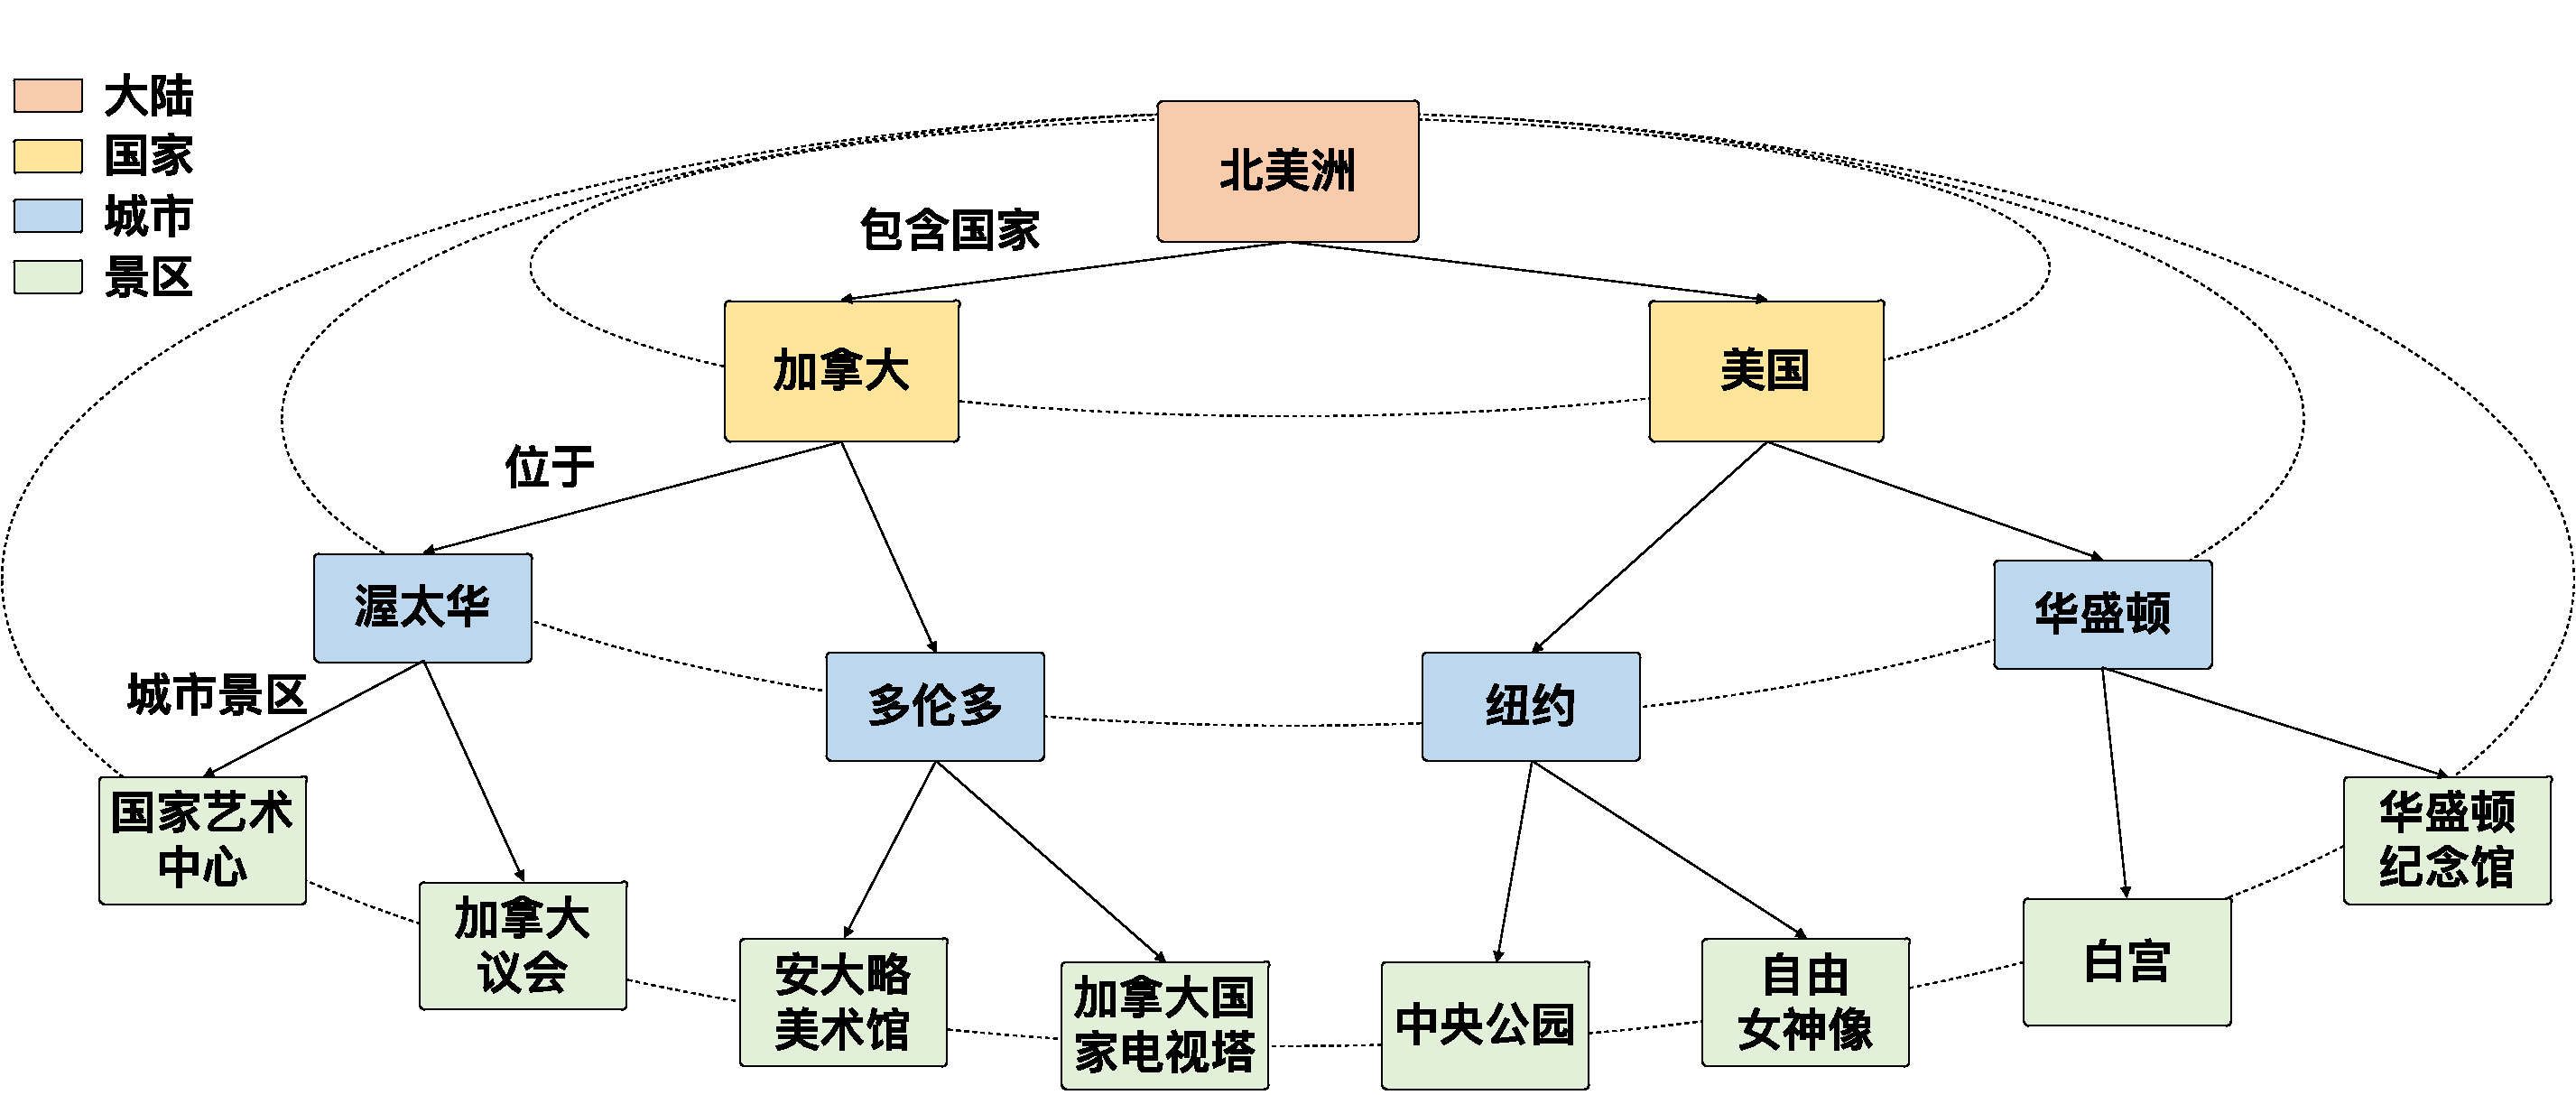
\includegraphics[width=1.0\textwidth]{1_KG}
  \caption{知识图谱}
  \label{1_KG}
\end{figure}

在实践中,知识图谱旨在作为组织或社区内不断发展的知识共享基础。知识图谱可以分为两类,分别是通用知识图谱和领域知识图谱~\cite{hogan2021knowledge}。两类知识图谱的原理相同,区别在于知识范围和应用领域,两种知识图谱在国内外均已得到广泛应用。国外的通用知识图谱包括百科知识图谱Freebase~\cite{bollacker2007platform},DBpedia~\cite{lehmann2015dbpedia}和Yago~\cite{hoffart2011yago2},多语言百科知识图谱Wikidata~\cite{vrandevcic2014wikidata},词典知识图谱WordNet~\cite{miller2007wordnet}和常识知识图谱CYC~\cite{lenat1995cyc}等。国内的通用知识图谱则包括中文百科知识图谱Zhishi.me~\cite{niu2011zhishi},该知识图谱首先采用固定的抽取规则,从百度百科、互动百科和中文维基百科中抽取实体信息,随后对不同百科的实体进行对齐,从而完成实体链接。CN-DBpedia~\cite{xu2017cn}是复旦大学开发的大规模通用领域结构化百科,从中文百科类网站的纯文本信息中提取信息,经过过滤、融合、推断等步骤后构成高质量结构化数据。领域知识图谱主要服务于特定行业领域,随着知识图谱在工业界的推广,逐渐发挥着越来越重要的作用。国外的领域知识图谱包括服务网络搜索的Google\footnote{https://blog.google/products/search/introducing-knowledge-graph-things-not/}知识图谱,服务社交网络的LinkedIn\footnote{https://engineering.linkedin.com/blog/2016/10/building-the-linkedin-knowledge-graph}知识图谱,服务商业领域的Aribnb\footnote{https://medium.com/airbnb-engineering/scaling-knowledge-access-and-retrieval-at-airbnb-665b6ba21e95}和Amazon\footnote{https://www.aboutamazon.com/news/innovation-at-amazon/making-search-easier}知识图谱,以及服务金融领域的Banca d’Italia~\cite{bellomarini2019knowledge}知识图谱等。国内的领域知识图谱包括百度~\cite{wang2013xlore}、淘宝~\cite{xu2021alime}、微博~\cite{wei2020analysis}等企业的知识图谱。由于领域知识图谱涉及到具体而复杂的领域场景,需要业务和开发专家的配合,因此对领域知识图谱的设计和开发提出了更高的要求。综上所述,知识图谱能够采用简洁的表示形式,将复杂多样的知识转化为清晰的三元组形式,并提供了强大的知识存储和推理能力,具有重要的研究和应用价值。

然而,知识图谱的知识信息通常采用自然语言进行描述,难以被计算机所处理和应用。因此,为了方便知识图谱的后续应用,需要将知识图谱内的知识信息转换为计算机能够直接处理的向量形式,这项技术被称为知识图谱表示学习(Knowledge Graph Representation Learning, KGRL)~\cite{chen2022rlpath}或知识图谱嵌入(Knowledge Graph Embedding, KGE)~\cite{wang2021transet}。知识图谱表示学习模型能够将知识图谱中的实体和关系映射到低维稠密的向量空间进行表示,同时保留其中的结构和语义信息,从而能够进行知识推理等知识应用工作。知识图谱表示学习主要涉及四个问题:(1)选择何种表示空间:现有的模型采用的表示空间可以分为欧氏空间~\cite{lu2022dense}、流形空间~\cite{ebisu2018toruse}、复向量空间~\cite{trouillon2016complex}和黎曼空间~\cite{pan2021hyperbolic}。(2)采用何种评分函数:现有的评分函数包括基于距离的评分函数~\cite{sachan2020knowledge}和基于语义相似度的评分函数~\cite{xiao2017ssp}。(3)应用何种编码模型:现有模型采用的编码模型包括线性模型~\cite{peng2020lineare}、双线性模型~\cite{pan2021hyperbolic}、因式分解模型~\cite{ji2015knowledge}和神经网络模型~\cite{jiang2021kernel}。(4)是否采用辅助信息,以及采用何种辅助信息:可以加入文本信息、视觉信息和类型信息等多种辅助信息~\cite{wang2017knowledge}。通过知识图谱表示学习,可以将知识信息转换为向量表示,作为知识图谱补全等下游任务的输入。由于知识图谱通常是采用自动或半自动的方式进行构建,因此通常是不完整的。通过现有知识预测知识图谱中缺失的知识,进行知识图谱补全,是提高知识图谱质量的有效手段~\cite{vu2019capsule}。同时知识图谱表示学习也能够通过简单的单跳知识推理,完成部分知识图谱问答工作,在智能问答等应用中具有重要价值。

尽管知识图谱表示学习能够完成部分知识图谱补全和知识图谱问答的工作,但无法对关系路径进行建模,而只能基于单个实体或者关系进行简单的补全或问答,如进行单跳知识图谱问答。同时,知识图谱表示学习通过向量计算的方法进行隐式的知识图谱补全,本质上属于黑盒模型,无法提供充分的证据,可解释性比较差。因此,需要借助知识图谱上的知识推理方法,综合考虑知识图谱网络图的拓扑结构信息对复杂关系路径进行建模,从而解决更为复杂的知识图谱补全和知识图谱问答内容,如实现多跳知识图谱问答,并提供相应推理证据~\cite{chen2020review}。知识推理不局限于传统的基于逻辑的和规则的推理方法,还可以采用更多样化的推理方法,随着技术的发展,一系列新的知识推理方法不断涌现,例如随机游走方法~\cite{jagvaral2020path}、路径排序方法~\cite{zhao2021target}、启发式方法~\cite{he2021heuristic}和神经网络方法~\cite{wang2018deep}等。丰富的知识图谱内容为知识推理技术的发展提供了新的机遇和挑战。

综上所述,知识图谱在人工智能应用中具有较大价值,面向知识图谱的表示学习技术有助于将知识图谱转化成易于处理和应用的知识图谱表示向量,并为下游任务提供充分的支持。知识推理是知识图谱智能应用的一个重要任务,深入研究该任务,有助于加深对知识图谱的认知,并充分和有效地利用知识图谱的知识。因此,本文旨在提出一种有效的知识图谱表示学习模型,随后基于知识图谱表示学习模型,实现一种知识推理模型,在适用于大规模知识图谱的前提下保证知识推理的质量,并能够解决诸如知识图谱补全、单跳知识图谱问答、多跳知识图谱问答和稀疏知识图谱上的知识图谱问答等知识推理任务。

\section{研究现状}
本节对面向知识图谱的表示学习和知识推理方法进行介绍,并介绍了一些常见的知识推理应用,此外还针对现有工作的问题进行了分析。

\subsection{知识图谱表示学习研究现状}
知识图谱能够有效地表示知识图谱中的结构化数据,但是难以被计算机进行直接处理和利用,需要先通过知识图谱表示学习的过程将知识三元组转换为向量的形式,才能应用于各类知识图谱推理任务。

知识图谱可以表示为$G=\{E, R, F\}$,其中$E$、$R$和$F$分别表示实体、关系和事实的集合。知识图谱内的事实三元组可以表示为$(h, r, t) \in F$,其中$h$、$r$和$t$分别表示头实体、关系和尾实体。例如,对于给定的事实三元组(\textit{美国,首都,华盛顿特区}),其中的\textit{美国}是头实体$h$,\textit{华盛顿特区}是尾实体$t$,\textit{首都}则是头实体和尾实体之间的关系$r$。同时根据定义,有$h \in E$,$t \in E$,$r \in R$,以及$(h, r, t) \in F$。经过知识图谱表示学习后,可以将知识图谱中的节点和关系映射到低维稠密向量空间中。
这里使用粗体字符表示知识图谱表示向量,并设置目标向量空间为$d$维的欧氏空间,则完成知识表示后的实体和关系向量有$\bm{e} \in \mathbb{R}^{\mathrm{d}}$和$\bm{r} \in \mathbb{R}^{\mathrm{d}}$。欧氏空间是一种常用的向量空间,在实际的知识图谱表示学习任务中需要根据模型的需要来设置向量空间。

为了构建知识图谱表示学习模型,需要完成三个步骤:(1)定义实体和关系在向量空间的表示形式。在这一步中,需要选择向量空间,设计编码模型,并确定是否需要辅助信息。(2)定义评分函数$f_r(h, t)$,用于评价知识$(h, r, t)$的合理性。知识图谱中可见事实三元组的得分一般会高于潜在事实三元组的得分。以及(3)学习实体和关系的表示,使知识图谱中可见事实三元组的总置信度最大化。

目前的知识图谱表示学习模型可以分为翻译模型,语义匹配模型和因果推断模型。

\subsubsection{翻译模型}
翻译模型采用基于距离的评分函数,将关系看做头实体和尾实体之间的翻译,并将关系翻译后两个实体之间的距离作为得分,进而实现衡量事实三元组的合理性。

翻译模型的典型代表是Bordes等人提出的TransE模型~\cite{bordes2013translating},其思想源于Mikolov等人提出的词嵌入模型word2vec~\cite{toms2013},在该模型中发现了词向量空间中存在平移不变性。例如TransE将知识图谱中的实体和关系映射到$d$维欧氏空间中,即$\bm{h}, \bm{r}, \bm{t} \in \mathbb{R}^{\mathrm{d}}$,并将关系看做是实体之间的连接向量,遵循$\bm{h} + \bm{r} \approx \bm{t}$,例如$\bm{h}$(\textit{美国}) $+ \bm{r}$(\textit{首都}) $\approx \bm{t}$(\textit{华盛顿特区})。同时对于给定三元组$(h, r, t)$,通过计算向量$\bm{h} + \bm{r}$和$\bm{t}$之间的$L1$或$L2$距离,进而得到三元组的合理性得分。对于较为合理的三元组,其得分应尽量接近0,对于不合理的三元组则希望其得分相对较低。TransE模型采用的得分函数可以表示为:$f_r(h, t) = - \|\bm{h} + \bm{r} - \bm{t}\|_{\ell_1 / \ell_2}$。尽管TransE模型在大规模知识图谱表示学习方面取得了巨大进步,但在处理如一对多、多对一和多对多等复杂关系时仍然存在困难。例如给定两个三元组(\textit{北京,所属国家,中国})和(\textit{上海,所属国家,中国}),可以发现它们是多对一类型的关系,即多个城市可以所属于同一个国家。根据TransE模型的要求$\bm{h} + \bm{r} \approx \bm{t}$,则实体\textit{北京}和\textit{上海}会被映射到向量表示空间中十分接近的位置。然而这两个实体实际上存在较大差异,因而这种映射是不合理的。

为了更好地处理复杂关系问题,Wang等人提出的TransH模型~\cite{wang2014knowledge}扩展了原始的TransE模型,为每种关系分别构建关系超平面,从而让一个实体在不同的关系超平面中会得到不同的表示向量。对于关系$r$,TransH会采用关系$r$独有的平移向量$\bm{d}_r$和超平面法线向量$\bm{w}_r$对关系进行表示。对于给定三元组$(h, r, t)$,TransH首先将$h$和$t$的表示向量沿着法线向量$w_r$的方向映射到关系超平面,设$\bm{h}_\perp$和$\bm{t}_\perp$分别为头实体和尾实体的映射向量,则有$\bm{h}_{\perp} = \bm{h} - \bm{w}_r^{\top} \bm{h} \bm{w}_r$,$\bm{t}_{\perp} = \bm{t} - \bm{w}_r^{\top} \bm{t} \bm{w}_r$。随后用关系平移向量$d_r$连接头实体向量和尾实体向量。TransH模型的评分函数为$f_r(h, t) = -\left\|\bm{h}_{\perp} + \bm{d}_r - \bm{t}_{\perp}\right\|_2^2$。虽然TransH模型使得实体能够根据关系获得不同表示,但全部实体和关系仍然在分布在相同的特征空间$\mathbb{R}^{\mathrm{d}}$中。由于实体具有多种语义,而不同关系可能关注实体的不同语义,因此单个特征空间可能不足以反映实体和关系的这一性质。

为了解决上述问题,Lin等人提出的TransR~\cite{lin2015learning}进一步扩展了TransH,将关系超平面扩展到了关系空间,即为每种关系构建对应的关系空间。对于给定三元组$(h, r, t)$,TransR将实体$h$和$t$映射到实体向量空间$\mathbb{R}^{\mathrm{d}}$中,同时为每个关系设置了相应的投影矩阵$\mathbf{M_r} \in \mathbb{R}^\mathrm{k \times d}$,能够将实体向量映射到关系$r$对应的向量空间$\mathbb{R}^{\mathrm{k}}$。设$\bm{h_\perp}$和$\bm{t_\perp}$分别为头实体和尾实体的映射向量,则有$\bm{h}_{\perp}=\mathbf{M}_r \bm{h}$,$\bm{t}_{\perp} = \mathbf{M}_r \bm{t}$。TransR采用投影矩阵,因此时空复杂度高于TransE和TransH。Ji等人提出的TransD~\cite{ji2015knowledge}模型很好地改善了TransR模型存在的问题。TransD对给定三元组$(h, r, t)$中每个实体和关系都构建两组向量,其中一组向量用来表示实体或关系的含义信息,表示为$\bm{h, t} \in \mathbb{R}^{\mathrm{d}}$和$\bm{r} \in \mathbb{R}^{\mathrm{k}}$,另一个向量用于形成两个动态投影矩阵,表示为$\bm{h_p, t_p} \in \mathbb{R}^{\mathrm{d}}$和$\bm{r_p} \in \mathbb{R}^{\mathrm{k}}$。相应地,构建的动态投影矩阵为$\mathbf{M}_{r h} = \bm{r}_p \bm{h}_p^{\top} + \mathbf{I}$,$\mathbf{M}_{r t}=\bm{r}_p \bm{t}_p^{\top} + \mathbf{I}$,其中$\mathbf{I} \in \mathbb{R}^{\mathrm{k \times d}}$是单位矩阵。设$\bm{h_\perp}$和$\bm{t_\perp}$分别为头实体和尾实体的映射向量,则有$\bm{h}_{\perp}=\mathbf{M}_{r h} \bm{h}$,$\bm{t}_{\perp}=\mathbf{M}_{r t} \bm{t}$。通过构建动态投影矩阵,TransD降低了矩阵运算的时空复杂度。

上述模型主要目标在于通过改变实体和关系的表示空间,提高表示学习的效果。除此之外,还有一些研究者从评分函数和编码方式的角度入手改进模型。对于给定的三元组$(h, r, t)$,TransM~\cite{fan2014transition}将与关系相应的权重$\theta_r$相关联,并将评分函数定义为$f_r(h, t)=-\theta_r\|\bm{h} + \bm{r} - \bm{t}\|_{1 / 2}$。通过给一对多、多对一和多对多关系分配较低的权重,可以让向量$\bm{h} + \bm{r}$和$\bm{t}$之间留有更大的距离。MainfoldE~\cite{xiao2016one}将$\bm{h} + \bm{r} \approx \bm{t}$的要求弱化为$\|\bm{h} + \bm{d} - \bm{t}\|_2^2 \approx \theta_r^2$,从而将$t$映射到以$\bm{h} + \bm{r}$为中心,半径为$\theta_r$的超球体,而不再是靠近$\bm{h} + \bm{r}$的确切点。同时,MainfoldE的评分函数定义为$f_r(h, t) = -\left(\|\bm{h} + \bm{r} - \bm{t}\|_2^2 - \theta_r^2\right)^2$。TransA~\cite{xiao2015transa}在TransR的基础上,使用自适应马氏距离代替传统的欧氏距离,并定义评分函数为$f_r(h, t) = -(|\bm{h} + \bm{r} - \bm{t}|)^{\top} \mathbf{M}_r(|\bm{h} + \bm{r} - \bm{t}|)$,从而使模型在处理复杂关系时更加灵活。

\subsubsection{语义匹配模型}
语义匹配模型采用基于相似度的评分函数,通过分析实体和关系的向量空间表示捕获语义信息,进而评估事实的合理性。模型的核心方法是,首先将知识图谱中的事实三元组$(h, r, t)$转换为三维的二元张量$\mathbf{X} \in \mathbb{R}^{\mathrm{n \times m \times n}}$,其中n为实体数量,m为关系数量,张量的每个切片$\mathbf{X}_k(k=1,2, \ldots, m)$对应相应的关系,张量值$\mathbf{X}_{i j k}$代表事实三元组$\left(h_i, r_j, t_k\right)$是否存在于知识图谱中,如果为1则存在,为0则不存在。

RESCAL~\cite{nickel2011three}是语义匹配模型的典型代表,采用张量来表示知识图谱的结构。对于关系$r_k$,有张量切片$\mathbf{X}_k \approx \mathbf{A} \mathbf{R}_k \mathbf{A}^{\top}$,其中矩阵$\mathbf{A}$用于捕获实体的潜在语义表示,矩阵$\mathbf{R}_k$用于对头尾实体对的交互进行建模。对于给定的三元组$(h, r, t)$,RESCAL的评分函数定义为$f_r(h, t)=\bm{h}^{\top} \mathbf{M}_r \bm{t}$,其中$\bm{h}, \bm{t} \in \mathbb{R}^d$是实体的嵌入向量,$\mathbf{M}_r \in \mathbb{R}^\mathrm{d \times d}$表示关系中的潜在语义信息。通过张量分解的方法,RESCAL能够较好地捕获实体和关系的语义信息,并给出三元组的合理性得分。然而,RESCAL的计算复杂度比较高。为了改善模型的时空复杂度,DistMult~\cite{yang2015embedding}将$\mathbf{M}_r$限制为对角矩阵,即$\mathbf{M}_r=\operatorname{diag}(\bm{r}), \bm{r} \in \mathbb{R}^\mathrm{d}$。随后,评分函数被调整为$f_r(h, t)=-\bm{h}^{\top} \operatorname{diag}(\bm{r}) \bm{t}$。通过这样的转换,DistMult显著降低了算法复杂度,同时在实验结果上取得了提高。然而,DistMult对头实体和尾实体的计算是对称的。对此,ComplEx~\cite{trouillon2016complex}模型通过复数嵌入,能够在不对称关系中扩展DistMult模型。实体和关系被嵌入到了复数空间$\mathbb{C}^\mathrm{d}$中,同时评分函数被修改为$f_r(h, t)=\operatorname{Re}\left(\bm{h}^{\top} \operatorname{diag}(\bm{r}) \bar{t}\right)$,其中$\operatorname{Re}(\cdot)$表示复数值的实数部分,$\bar{t}$表示尾实体的复数共轭部分。通过该评分函数,具有不对称关系的三元组就可以根据实体的序列获取不同的分数。

另一种具有代表性的语义匹配模型是RotatE~\cite{sun2018rotate}。受欧拉恒等式$e^{i \theta}=\cos \theta + i \sin \theta$的启发,RotatE引入了旋转哈达玛积,它将关系视为复数空间中头实体到尾实体的旋转,对于给定的三元组$(h, r, t)$,RotatE的评分函数为$f_r(h, t) = \|\bm{h} \circ \bm{r} - \bm{t}\|$,其中$\circ$表示旋转哈达玛积。通过这种方式,RotatE具有较好地表示和推理能力,能够处理对称/反对称关系、自反关系和复合关系。然而,RotatE采用的旋转哈达玛积在处理部分三元组时存在局限性。例如,给定三元组(\textit{母亲},\textit{父亲},\textit{祖母})和(\textit{父亲},\textit{母亲},\textit{祖父}),RotatE计算时会判断\textit{父亲的母亲}与\textit{母亲的父亲}是逻辑等价的,并将\textit{祖母}和\textit{祖父}映射到向量空间中角度接近的位置,但这种推导显然是错误的。为了解决这一问题,QuatE~\cite{zhang2019quaternion}模型将RotatE从复数空间扩展到四维空间,并采用哈密尔顿积替换旋转哈达玛积,用于捕获实体和关系间的潜在语义关联。相应的评分函数为$f_r(h, t)=\bm{h} \otimes \bm{r}|\bm{r}|^{-1} \cdot \bm{t}$,其中$\otimes$表示哈密尔顿积。由于哈密尔顿积的前后算子不可交换,所以能够区分类似\textit{父亲的母亲}和\textit{母亲的父亲}这样的实体概念,从而较好地解决RotatE存在的问题。

\subsubsection{因果推断模型}
因果推断模型将因果推断方法引入知识图谱表示学习领域,主要思想是引入因果干预方法,增强模型的领域适应性,减少局部结构差异,从而提高模型的泛化能力。同时通过因果分析还能够确定知识图谱表示学习时哪些特征信息有助于进行实体和关系表示,并提高相应的信息权重,进而增强模型的表示效果。

Wang等人提出的NIC模型~\cite{wang2021neighborhood}将因果推断模型与知识图谱表示学习领域相结合,提高了表示效果。知识图谱表示学习模型通过设计表示空间、评分函数和编码模型,并考虑加入辅助信息,完成模型的构建。对于给定的三元组$(h, r, t)$,模型会通过评分函数$f_r\left(h, t\right)$给出三元组的合理性评分。在训练模型学习实体和关系的向量表示时,通常选择优化目标是使得知识图谱中已有三元组的评分尽可能比未出现的三元组评分更高。然而,训练过程中的评分主要用于进行结果排序,而不是作为三元组的置信度得分。这导致评分函数的效果下降,限制了知识图谱补全等知识推理工作的发展。例如,给定三元组$(h, r, t)$,常规知识图谱表示学习方法的评分函数$f_r\left(h, t\right)$得到相应评分为0.9,但该三元组的实际置信度得分只有0.3,即评分与置信度得分存在不匹配的问题。因此,为了解决上述问题,使得评分函数能够给出接近实际置信度的评分,NIC提出了一个基于因果干预的置信度评估方法,称为邻里干预一致性(Neighborhood Intervention Consistency,NIC),通过验证预测结果的稳定性来评估置信度分数,具体方法是调整实体向量在不同维度上的值,设置为集合$\{0, \operatorname{avg}(\bm{e}), \max (\bm{e}), \min (\bm{e})\}$中的任意一种,即可以取零值、平均值、最大值和最小值其中之一。如果调整所有特征中的权值会导致时间效率过低,因此NIC通过特征选择获取不同维度的贡献,贡献计算函数为$w_j=|E|^{-1} \sum_{i=0}^{|E|}\left(\mathbf{E}_{i, j}-\operatorname{avg}\left(\mathbf{E}_{:, j}\right)\right)^2$,并选择贡献最大的维度进行调整。完成调整后,观察模型的输出序列是否改变或者是否与原始序列匹配,匹配度计算方法为$\zeta\left(S, S^{N_i}\right)=\sum_{j=0}^J \sigma(S)_j\left(1-\operatorname{Sgn}\left(\left|\varrho(S)_j-\varrho\left(S^{N_i}\right)_j\right|\right)\right)$,其中$\sigma$和$\operatorname{Sgn}$分别为Softmax函数和Sign函数,该函数可以表示因果干预后预测结果的稳健性,并计算置信度得分为$p_{n i c}(S)=d^{-1} \sum_{i=0}^d\left(\varsigma\left(S, S^{N_i}\right)\right)$,是0到1之间的实数。

另一种具有代表性的因果推断知识图谱表示学习模型为Feng等人提出的CGI模型~\cite{feng2021should},采用图卷积神经网络。图卷积神经网络广泛应用于知识图谱表示学习中,其主要思想是通过聚合实体节点的邻域信息实现实体表示效果的增强。然而,由于知识图谱中局部结构属性存在较大差异,即存在局部结构差异问题,从而造成实体节点表示存在不一致分布的问题,这导致对不同节点使用相同的聚合方法会降低节点表示效果。通常的解决方案是采用注意力机制,通过训练降低可能导致局部结构差异的邻居的权重,然而通常无法实现理想情况的注意力机制效果。针对上述问题,CGI采用了因果图卷积神经网络模型,该模型能够根据局部结构的因果效应调整训练好的图卷积神经网络模型。CGI首先得到节点的原始表示向量,该向量受到邻域特征和自身特征的影响。随后采用因果干预,将邻域置位空,从而实现屏蔽图结构,并要求实体节点根据自身特征获取表示向量。因果干预过程可以表示为$e=f(x, \mathcal{N}(x) \mid \theta)-f(x, \operatorname{do}(N=\emptyset) \mid \theta)$,其中$\operatorname{do}(N=\emptyset)$表示执行因果干预,将邻域置为空集合。最后CGI根据局部结构的因果效应、预测置信度和其他因素,采用一个独立的二元分类器$D=\{(x, p) \mid \hat{z}=z \cup \hat{z}=z\}, p=\operatorname{flag}(\hat{z}=z)$,在因果干预表示和原始表示之间进行选择。实验证明模型通常能够在遇到局部结构差异时选择因果干预表示,即屏蔽邻域特征仅采用节点自身特征的表示。

\subsection{知识推理研究现状}
通过知识图谱表示学习模型可以通过知识图谱问答的方式实现知识推理,即给定查询语句,通过知识抽取技术获取对应的查询三元组$\left(h, r, ?\right)$,$\left(h, ?, t\right)$或$\left(?, r, t\right)$,通过将知识图谱内所有关系或实体作为候选答案,输入到知识图谱表示学习模型中,从而将实体与关系映射到低维向量空间中,并通过得分函数进行打分,随后根据得分结果进行排序,选择得分最高的实体或关系作为答案,并完成知识推理。然而,基于知识表示学习模型的推理在形式上只能完成单跳的推理,无法显式地进行多跳推理,因而无法提供推理路径。这使得推理过程缺乏可解释性~\cite{wang2019deeppath}。为了解决这一问题,提出了关系路径推理方法,该类方法利用知识图谱上的拓扑结构信息,在知识图谱的关系路径上进行建模和推理。采用关系路径推理的方式,不仅可以得到推理结果,同时还可以给出一个可解释的、采用推理路径作为引导的推理过程。

现有的知识推理模型可以分为符号逻辑推理模型,神经推理模型和神经符号混合推理模型。

\subsubsection{符号推理模型}
符号推理模型(Symbolic reasoning model)旨在为非结构化自然语言查询语句生成结构化的查询。现有的符号推理模型可以分为语义解析和基于模板的知识推理两种方法。其中语义解析方法通过自然语言处理工具将问题转换为句法依赖表示。基于模板的知识推理方法则构建大量模板,包括自然语言模式和相应的结构化查询模式(例如SPARQL),从而实现复杂问题的分解。

马尔可夫符号网络(Markov Logic Network, MLN)~\cite{richardson2006markov}是基于预定义的规则和知识图谱中的事实三元组信息构建的概率图模型,能够在模型训练的过程中学习不同规则的权重,最终。具体而言,给定一个具体的规则集合,其中的每个规则都可以通过知识三元组进行具体查询,则可以通过下列步骤完成MLN模型的构建:首先为每个规则对应的知识三元组构建一个对应节点,如果知识三元组存在则节点值设为1,否则设为0。随后如果两个节点如果对应同一个规则,则在两个节点之间构建一条边。最后令每个规则对应一个特征,如果规则成立则特征值为1,否则特征值为0。规则的所有节点都共享这个特征。完成MLN模型构建后,网络中所有节点的联合分布定义为$P(X=x)=Z^{-1} \exp \left(\sum_i w_i n_i(x)\right)$,其中$w_i$是对应规则的权重,是$n_i$规则对应节点的数量。随后可以通过MCMC算法进行MLN模型的推理,并通过优化伪似然度量实现权重的学习。基于学习的权重,即可以完成具体的路径推理。通过引入权重信息,MLN能够较好地将一阶谓词逻辑和概率图模型进行结合,并实现不确定性的推理。然而,知识图谱结构十分复杂,造成了MLN的推理非常困难且效率低下。此外,知识图谱中缺失的三元组也会影响规则推理的效果。为了解决上述问题,pLogicNet~\cite{qu2019probabilistic}综合了MLN和图嵌入技术的思想,首先通过MLN定义知识图谱中事实三元组的联合分布,并对每种逻辑规则与权重构建关联,随后采用变分EM算法有效地学习权重。在EM算法中,E步骤推断未观察到的三元组的合理性,其对应的变分分布采用TransE等知识图谱表示学习模型进行参数化,M步通过优化观察到的三元组和知识图谱表示学习模型得到的三元组上的伪似然来更新逻辑规则的权重。通过上述方法,pLogicNet可以实现高效知识推理,同时能够处理知识图谱中缺失的信息。

另一类符号逻辑推理模型的代表是ProbLog~\cite{de2007problog},它是逻辑编程语言ProLog的一个改进。ProLog能够基于给定规则、事实和查询语句进行自动的知识推理并给出答案。ProbLog则是对于每种规则设置了一个概率,并令最终的知识推理给出推理的概率,从而模拟知识推理过程中的不确定性。给定查询,则推理概率被定义为$P\left(q \mid T\right)=\sum_{L \in L_T} P(q, L \mid T)$,其中T描述了原因L的概率分布,因此推理概率被分解为查询的所有联合概率和每种可能的原因集合的总和。其中有$P(q, L \mid T)=P(q \mid L) \cdot P(L \mid T)$,进一步分解了推理概率,其中$P(L \mid T)$表示给定原因的情况下查询的概率,如果至少有一个答案能够使查询为真,则对应的$P(L \mid T)$的值为1。式中另一项,即原因集合的概率的计算方法为$P(L \mid T)=\prod_{c_i \in L} p_i \prod_{c_i \in L_r \backslash L}\left(1-p_i\right)$。为了计算$P(L \mid T)$,一种方法是枚举所有可能的逻辑规则和对应的事实,效率较低。另一种方法是采用ProLog的选择线性确定(Selective Linear Definite,SLD)方案,采用自上而下的方式构造SLD树。首先通过查询步骤初始化根节点,随后通过应用每个规则及对应的事实来递归创建子目标,到达结束条件时停止迭代,即找到了查询目标或到达了树的最大深度。同时,每种查询结果都与一系列带有概率的规则相关联。

\subsubsection{神经推理模型}
神经推理模型的推理方法是将知识图谱中的实体、关系和查询问题共同编码到相同的表示空间中,并在表示空间中进行知识推理。传统的基于距离和基于语义匹配的模型无法满足知识推理的要求,为了获得更加有效的实体和关系嵌入效果,神经推理模型引入了神经网络结构,用于知识图谱邻域信息的建模。神经推理模型与知识图谱表示学习模型比较相似,都是首先进行知识图谱表示,随后实现知识推理等任务,但不同在于,神经推理模型会将自然语言查询问题也编码到表示空间中,从而增强知识推理的效果。同时,神经推理模型能够处理单跳知识图谱问答、多跳知识图谱问答和复杂逻辑问答问题,而知识图谱表示学习模型通常只能处理单跳知识图谱问答问题。

ConvE~\cite{dettmers2018convolutional}是第一种采用卷积神经网络的神经推理模型,首先将头实体和关系映射到向量空间,随后将向量转换成矩阵并进行拼接,输入到卷积层中。ConvE采用二维卷积捕获两个实体之间的特征交互信息,并通过卷积层和全连接层获取实体之间不同维度的局部信息,返回特征图张量。随后,将张量转化为向量,并投影到向量空间,最后通过计算与尾实体向量的内积,得到最终的合理性得分。其评分函数为$f_r\left(h, t\right)f(\operatorname{vec}(f([\bm{h} ; \bm{r}] \times \omega)) \mathbf{W}) t$,其中$\omega$为卷积核,$\mathbf{W}$为权重矩阵。此外,ConvE还引入了一个一对多的评分程序,能够自动匹配所有尾实体,从而能够更有效率地评估所有候选答案尾实体。然而,ConvE将实体和关系向量转换为矩阵并进行拼接,这一过程丢失了翻译模型的平移不变性。对此,ConvKB~\cite{nguyen2018novel}去除了ConvE的转换操作,并采用一维卷积保持平移不变性,同时捕获实体之间的全局关系和平移特征。ConvKB将每个三元组$(h, r, t)$的d维度嵌入表示为一个三列的矩阵$(\bm{h}, \bm{r}, \bm{t}) \in \mathbb{R}^{\mathrm{d} \times 3}$,随后将矩阵输入到卷积层,其中提供许多相同维度的过滤器,能够提取三元组中相同维度特征之间的全局关系,并通过对矩阵的每行进行操作以获得不同的特征图,最后将这些特征图拼接成一个三元组特征向量,并通过和权重矩阵进行点积运算得到最终的三元组合理性得分,评分函数为$f_r(h, t)=\operatorname{concat}(g([\bm{h}, \bm{r}, \bm{t}] \times \Omega)) \cdot \mathbf{W}$,其中$g$为激活函数,$\Omega$为过滤器,$\mathbf{W}$为权重矩阵。HypER~\cite{balazevic2019hypernetwork}是基于ConvE提出的又一种卷积神经网络推理模型,采用基于ConvE的超网络为每个关系生成卷积滤波器权重,超网络可以实现跨层的权重共享,并动态生成给定输入的权重。HypER使用基于特定关系的一维卷积滤波器来处理实体嵌入,这简化了嵌入模式。同时,HypER使用卷积算子实现头实体嵌入和一组特定于关系的滤波器$F_r$,滤波器是超网络$H$从关系嵌入中创建的,超网络的结构是一个全连接层。最后,HypER还应用了ReLU激活函数的权重矩阵$\mathbf{W}$实现特征图张量的向量化。HypER的评分函数为$f_r(h, t)=f\left(\operatorname{vec}\left(\bm{h} \times F_r\right) \mathbf{W}\right) \bm{t}$,相较于ConvE,HypER具有更强的表达能力和更少的参数。

传统的神经推理模型通过单向关系路径或文本信息引入上下文信息,而忽略了实体之间的各种连接模式,以及不重要的路径和词的影响,这造成模型无法充分捕捉三元组之间的关系信息。为了解决这一问题,R-GCN~\cite{schlichtkrull2018modeling}采用关系图卷积网络,显式地对多关系知识图谱进行建模并捕获实体周围的单跳邻域事实信息。R-GCN由编码器和解码器构成,在对实体进行编码的时候,R-GCN能够综合考虑实体连接之间的各类输入和输出的关系信息,并对实体的结构信息进行充分的编码。实体表示被更新为$\bm{h}_i^{(l+1)}=\sigma\left(\sum_{r \in R} \sum_{j \in \mathbf{N}_i^r} c_{i, r}^{-1} \mathbf{W}_r^{(l)} \bm{h}_j^{(l)}+\mathbf{W}_0^{(l)} \bm{h}_i^{(l)}\right)$,其中$\mathbf{N}_i^r$是节点i在关系$r \in R$下的邻域,$c_{i,r}$是特定问题的归一化常数。解码时,可以通过基数分解和块对角矩阵分解的方法求解,并选择DistMult分解模型作为评分函数,认为每个关系都对应一个对角矩阵,从而得到最终的评分函数为$f_r(h, t)=\bm{h}^T \mathbf{R}_r \bm{t}$。R-GCN分析了知识图谱中邻域信息对实体表示的影响,但是没有显式地对实体间的关系进行建模。SACN~\cite{shang2019end}模型对R-GCN进行了改进,是一种加权的GCN模型,能够同时考虑节点间的连通性、节点的属性和关系类型。SACN同样由编码器和解码器构成。编码器部分,SCAN引入了不同类型关系的权重以对GCN模型进行改进,得到加权图神经网络。同时,在聚合信息时对不同类型的关系分别进行聚合,因此可以将多关系图按照多个单关系图的形式进行分析。此外,SACN还将实体属性作为属性节点加入到了实体表示部分,并采用类似的方法进行分析。在SACN模型中,实体表示被更新为$h_i^{l+1}\sigma\left(\sum_{j \in \mathbf{N}_i} \alpha_t^l \bm{h}_j^l \mathbf{W}^l+\bm{h}_i^l \mathbf{W}^l\right)$。解码器采用Conv-TransE进行解码,利用卷积过滤器直接对相同维度的实体和关系向量进行处理。

\subsubsection{神经符号推理模型}
神经符号推理模型(Neural-symbolic reasoning model)是符号推理模型和神经推理模型的结合,综合了两种模型的优点。现有的神经符号推理模型包括神经增强符号推理模型(Neural-enhanced symbolic reasoning model)和端到端推理模型。其中,神经增强符号推理模型仅仅用于将问题解析成结构化的查询,随后需要使用查询方法才能够得到最终答案。而端到端推理模型可以自动完成解析问题并检索答案的步骤。

DeepPath~\cite{wang2019deeppath}首先将强化学习模型应用到了关系路径知识推理方面,并开发了一种新的奖励函数,通过综合分析模型是否到达目标节点、模型推理路径长度是否过长和与已有路径嵌入向量的相似度,来提高准确性、路径多样性和推理效率。DeepPath首先采用翻译模型的方法,对连续空间中的智能体状态信息进行编码,并选择知识图谱的关系空间作为强化学习模型的动作空间。另一种基于强化学习的模型是MINERVA~\cite{das2018go},根据基于LSTM的策略网络对邻域信息进行采样。同时,与DeepPath不同的是,MINERVA中的状态是由查询关系和部分路径的嵌入组成,在采样的过程中不需要答案实体的嵌入向量,从而能够允许MINERVA直接通过知识推理得到答案。同时,MINERVA还为知识图谱的每个节点增加了自关系,从而能够在推理过程中在到达答案实体时自动停止。然而DeepPath和MINERVA在分析模型是否到达目标节点时,提供的奖励机制比较简单,即如果智能体到达目标节点则提供值为1的奖励,同时对没有达到目标节点的情况提供值为-1的惩罚或者值为0的奖励。这种方法导致了奖励稀疏问题并降低了模型探索路径的效果。对此,Multi-Hop模型~\cite{lin2018multi}改进了强化学习的奖励函数,将硬奖励替换成了基于真实答案实体和推理实体之间相似度的软奖励。同时,受到dropout技术的启发,Multi-Hop在模型训练的过程中丢弃了一些动作,从而避免选择大量重复路径,缓解过拟合问题。另一种缓解奖励稀疏的方法由M-Walk~\cite{shen2018m}模型提出,该模型采用了一种基于价值的强化学习方法,并使用蒙特卡洛树搜索(Monte Carlo Tree Search,MCTS)来客服奖励稀疏的问题。具体而言,M-Walk迭代地使用MCTS的轨迹生成步骤和策略改进步骤,实现细化策略网络,从而获得更多的奖励信息。

除去关系路径知识推理模型,另一种神经符号推理模型采用图结构进行推理。GraIL模型~\cite{teru2020inductive}采用图神经网络的形式,并在提取的子图上推理两个实体之间的关系。具体而言,GraIL首先提取头实体和尾实体周围的k跳子图并取交集,随后采用元组$(d(i, h), d(i, t))$标记子图中的实体,其中$i$表示子图中的第$i$个节点,$d$表示头实体和尾实体到节点的最短距离。随后采用基于注意力的多关系图神经网络,也就是R-GCN,计算每个节点的实体表示,最后将头实体、尾实体和查询关系的表示向量连接起来,并以此为基础在子图上进行推理。GraIL在学习与实体无关的关系语义方面具有很强的能力。CogGraph~\cite{du2019cognitive}从给定的头实体和查询关系开始,通过策略网络在每一步扩展多个实体,随后采用GNN模型获取节点在推理子图中的表示向量,并预测答案。DPMPN模型~\cite{xu2019dynamically}采用了两个图神经网络模型来执行推理。第一个模型在整个知识图谱上进行消息传递,用于提供实体表示。第二个模型在查询子图上修建消息传递图,用于捕获与查询相关的语义。

此外,还有基于矩阵的神经符号推理模型。这种模型可以看做图神经网络模型的扩展,其不会基于跳数选择邻居,而是综合软注意力分数来评估不同邻居的重要性。其基本思想是通过矩阵运算来表达头尾实体之间的重要性。TensorLog~\cite{cohen2016tensorlog}是较早提出的基于矩阵的模型,能够通过知识推理,得到带有权重的链式逻辑规则,从而解释知识图谱中的每个关系。随后基于推理得到的规则,输入头实体和关系,目标是通过检索对实体进行排名,将正确答案尽可能排在靠前的位置。TensorLog采用独热向量表示实体,并用矩阵表示知识图谱中的向量,其中如果知识存在于知识图谱中,则矩阵对应位置为1。但是,TensorLog中的参数较难学习,因为每种规则都对应一个参数,而枚举规则本身就是一个离散的任务。对此,神经逻辑编程(NeuralLP)模型~\cite{yang2017differentiable}将规则的权重参数分解为了规则中谓词的权重。同时,设计了一个循环公式来动态建模规则的长度。最后,NeuralLP计算所有向量的加权平均值,并使用注意力来控制规则的长度。上述两种方法可以学习一些概率链式逻辑规则,但是无法推断出一些复杂的规则形式,如树状规则。此外,链式规则是基于特定的头实体进行推断的,这也会降低学习的泛化性。对此,神经逻辑归纳学习(Neural Logic Inductive Learning, NLIL)模型~\cite{yang2019learn}将原始语句进行合并以处理非链式规则,并取得较好的效果。

\subsection{知识推理应用}
通过知识图谱表示学习模型,可以得到知识图谱内实体和关系的表示向量。随后通过知识推理模型,可以进一步利用知识表示向量内的信息,从而实现一系列知识推理应用。常见的知识推理应用主要包括知识图谱补全和知识图谱问答。

\subsubsection{知识图谱补全}
知识图谱补全(Knowledge Graph Completion,KGC)~\cite{vu2019capsule}指的是预测与实体有相应关系的实体的任务,即给定头实体$h$和关系$r$预测对应的尾实体$t$,或是给定关系$r$和尾实体$t$预测对应的头实体$h$,前者可以表示为查询三元组$\left(h, r, ?\right)$,后者可以表示为查询三元组$\left(?, r, t\right)$,这种类型的知识图谱补全任务被称为实体预测。类似的,另一种知识图谱补全任务是给定头实体$h$和尾实体$t$并预测关系$r$,可以表示为查询三元组$\left(h, ? t\right)$,这种知识图谱补全被称为关系预测。以查询尾实体为例,给定查询三元组$\left(h, r, ?\right)$,首先选择在知识图谱表示学习模型,将头实体$h$和关系$r$映射到向量空间中,随后可以选择将知识图谱中每个实体作为候选答案,并使用得分函数$f_r\left(h, t\right)$计算三元组得分。随后,将按照得分从高到低的顺序获取候选答案的有序序列,并检查正确答案在序列中的位置。评价知识图谱补全的好坏主要在于正确答案在最终候选答案序列中的位置是否靠前,通常采用的评价指标有平均排序MR(正确答案排名的平均值)、平均倒数排序MRR(正确答案排名倒数的平均值)以及Hits@K(正确答案在序列中排名位于前K的比例)等。

\subsubsection{知识图谱问答}
知识图谱问答(Knowledge Graph Question Answering,KGQA)包括单跳知识图谱问答、多跳知识图谱问答和复杂逻辑问答等多种形式~\cite{saxena2020improving}。其中,单跳知识图谱问答与知识图谱补全类似,两者的区别在于,知识图谱补全采用查询三元组的形式,提供两个已知元素并要求模型通过推理得到未知的元素,从而实现知识图谱补全。知识图谱问答则不提供查询三元组,而提供自然语言查询语句$q$,并要求模型基于该问句进行问题的解答,答案类型可以是实体和关系。相比之下,多跳知识图谱问答更加复杂,知识推理模型需要通过知识图谱上的多跳关键路径进行推理才能获得答案实体和关系,同时部分多跳问答数据集如HotpotQA还要求模型提供相应的证据来证明推理的有效性~\cite{yang2018hotpotqa}。复杂逻辑问答提供的查询语句中包含多个主题实体,主题实体之间通过连接词$\land$、析取词$\vee$和否定词$\neg$进行聚合,因此可以对每个主题词进行多跳推理,最后对推理结果进行求交集,获取最终答案。知识图谱问答的常见解决方案是,首先对查询语句$q$进行实体识别,获取其中的主题实体,随后基于主题实体,可以采用知识图谱补全的方案,通过知识图谱表示学习模型进行单跳知识推理,或采用基于关系路径的知识推理模型进行多跳知识推理和复杂逻辑推理,最终得到目标实体或关系,实现问题求解。评价知识图谱问答的效果可以分析正确答案在最终答案候选序列的位置是否靠前,可以采用的评价指标有平均排序MR、平均倒数排序MRR和Hit@K等。


\subsection{存在问题分析}
随着DBpedia、Freebase和Yago等一系列大规模知识图谱的提出,面向知识图谱的表示学习和知识推理的相关研究取得了重要进展。然而,尽管越来越多的模型在各种知识推理应用中取得了瞩目的效果,但仍然面临着许多挑战:

\begin{itemize}
  \item [1)]\textbf{模型对知识图谱层次信息的感知能力不强:}现有面向知识图谱的表示学习和知识推理模型通常能够较好的建模知识图谱内部三元组的语义信息,但是通常对知识图谱的层次信息建模能力较差,导致在进行知识图谱表示和知识推理的过程中无法充分利用知识图谱内丰富的层次信息,限制了模型效果。
  \item [2)]\textbf{模型可解释性较差:}采用神经网络结构的知识推理模型由于模型结构属于黑盒模型,所以难以分析模型通过知识推理得出结果的具体过程。同时如果采用知识图谱表示学习模型直接进行知识推理,则模型只会得出推理结果,而不会提供相应的推理路径和证据信息,这导致难以分析模型推理具体过程并进而优化模型。
  \item [3)]\textbf{知识图谱表示学习模型与知识推理模型的结合不够充分:}由于通常情况下知识图谱表示学习模型与知识推理模型的训练过程相互分离和缺乏协作,导致模型间的结合不够充分,从而降低了面向知识图谱的知识推理的效果。
  \item [4)]\textbf{模型在复杂知识推理任务上的推理能力不足:}稀疏知识图谱上的知识推理任务和多跳推理任务在现实世界中十分常见,具有重要的研究和应用价值。然而现有的知识推理模型在面对上述复杂推理任务时表现仍然较差。同时,直接采用知识图谱表示学习模型只能实现单跳推理,这限制了知识图谱表示学习模型在知识推理任务上的进一步应用。
\end{itemize}

\section{论文工作}
本文提出了基于图神经网络的知识图谱表示学习模型NORMAN(k\textbf{NO}wledge graph \textbf{R}epresentation learning \textbf{M}odel based on gr\textbf{A}ph \textbf{N}eural network)和基于双重智能体强化学习的知识推理模型LAURA(know\textbf{L}edge graph re\textbf{A}soning model based on d\textbf{U}al-agent \textbf{R}einforcement le\textbf{A}rning)。

NORMAN模型首先采用基于极坐标系的编码器对知识图谱进行编码,从而捕获知识图谱中的层次信息,并将获取到的知识向量输入给图神经网络模型。随后通过图神经网络模型构建邻域子图并进行消息传递,从而捕获知识图谱中的邻域信息,并完成知识向量的更新。训练后得到的NORMAN模型能够将知识转换为向量形式,并可以为知识推理过程提供支持。
LAURA模型利用NORMAN模型提供的层次信息和得分函数,训练两种分别能获取实体和层次信息的强化学习智能体,并通过协作动作空间、协作策略网络和协作奖励实现两种智能体的信息交互和轨迹协调,最终完成知识推理模型的训练。得到的模型可以根据给定知识信息进行推理,返回知识推理结果、推理路径和推理置信度等信息。

\begin{figure}[t]
  \centering
  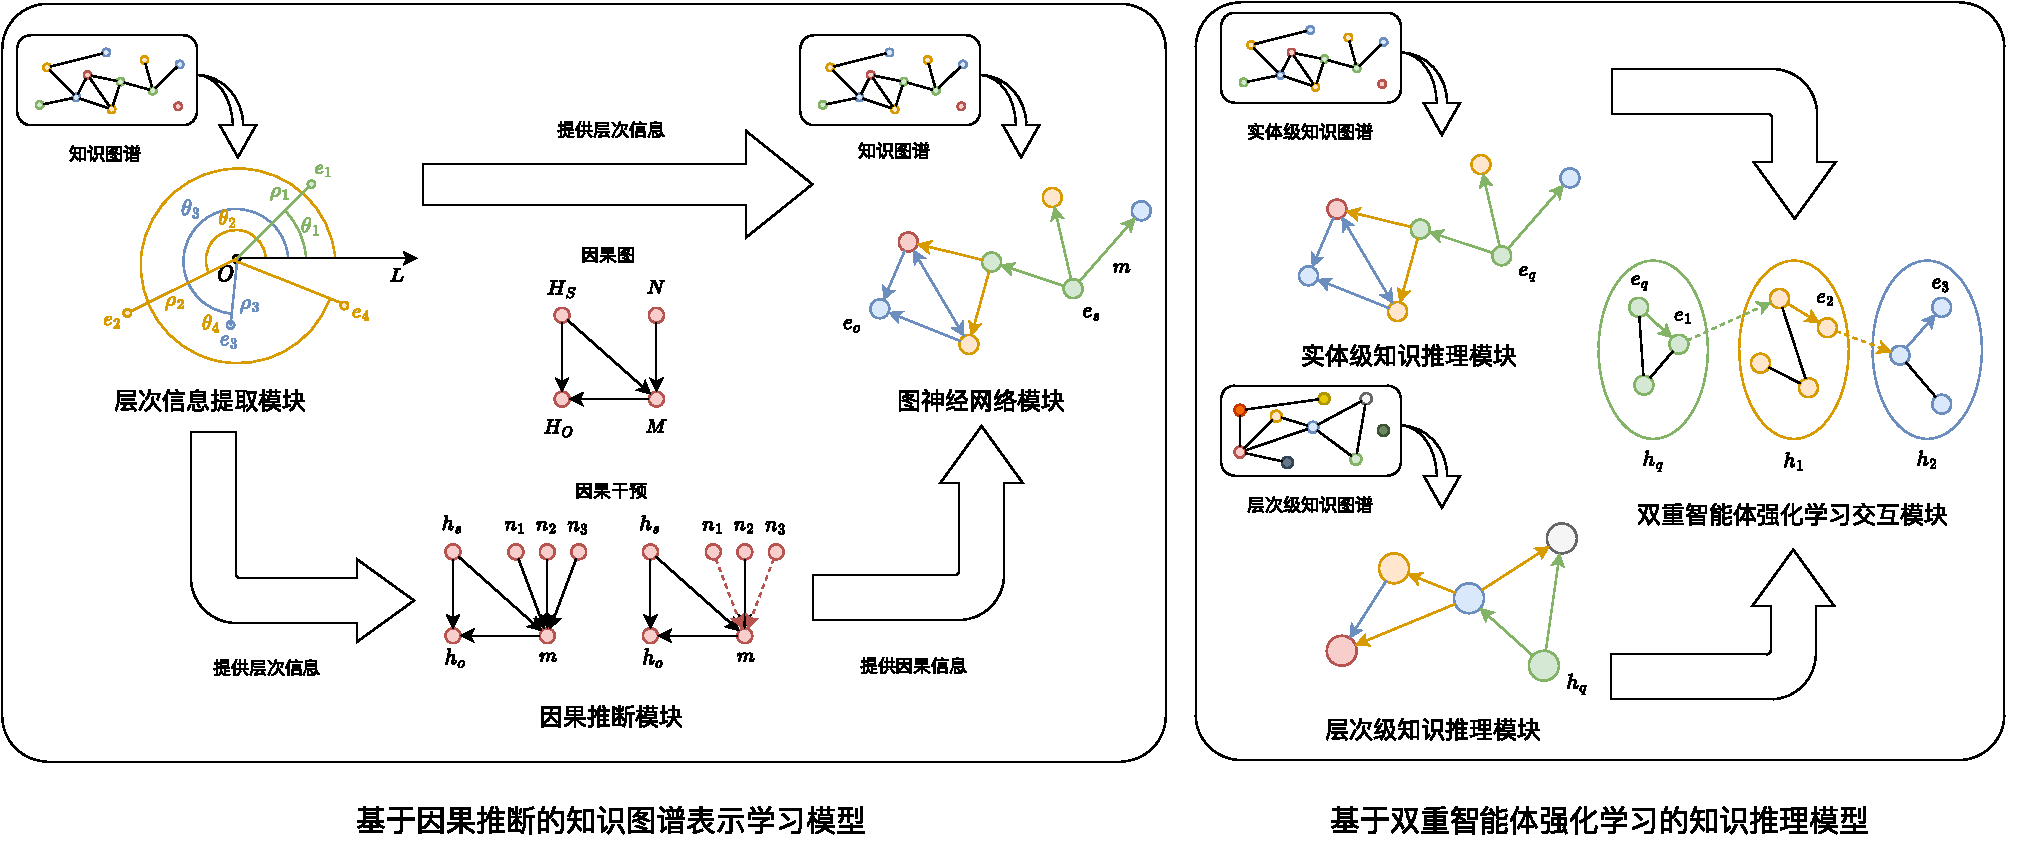
\includegraphics[width=1.0\textwidth]{1_Total}
  \caption{技术路线图}
  \label{1_Total}
\end{figure}
图\ref{1_Total}是本文的整体研究技术框架,具体研究内容如下:
\begin{itemize}
  \item [1)]\textbf{提出一种基于图神经网络的知识图谱表示学习模型NORMAN:}
  该方法主要针对知识图谱的层次信息和邻域信息进行建模,主要包含层次信息提取和图神经网络模型两部分。
  首先为了捕获知识图谱中的层次信息并对不同的实体和关系进行区分,提出了一种基于极坐标系的编码器。该编码器能够将知识编码为极坐标向量的形式,其中半径坐标向量用于捕获知识的层次信息,角坐标向量则用于区分不同类别的知识。
  随后为了捕获知识图谱中的邻域信息,提出了一种图神经网络模型。该模型首先利用层次信息提取过程得到的向量通过一个全连接层映射获取模型的初始向量,随后通过递归方式实现邻域子图构建和消息传递,并通过消息聚合函数将邻域子图中的消息聚合起来,通过信息更新函数将消息与节点向量相结合,实现节点信息更新。同时在消息传递过程中,对各个邻域节点的消息采用注意力机制,从而区分不同节点的消息贡献程度。
  通过上述方法,NORMAN模型能够有效地捕获知识图谱中的层次信息和邻域信息,进行高质量的知识表示,并能够在知识图谱补全等下游任务中进行应用。
  在多个公开数据集上的实验结果表明,本文提出的NORMAN模型在知识图谱补全任务上优于现有模型。
  \item [2)]\textbf{提出一种基于双重智能体强化学习的知识推理模型LAURA:}
  该方法主要针对知识图谱中的实体和层次信息进行建模。
  首先为了提高知识推理的可解释性,采用了强化学习框架,能够根据知识图谱中的拓扑结构进行多跳推理并生成推理路径,从而实现高可解释性的知识推理。
  随后为了保证知识推理路径的充分性,提出了一种新颖的双重智能体强化学习方法。在知识推理过程中构建了两种能够相互协作进行知识推理的强化学习智能体,两种智能体能够分别根据知识图谱中的实体和层次信息进行知识推理。同时,采用协作动作空间、协作策略网络和协作奖励等方法,能够帮助两种智能体实现信息交互,指导两种智能体沿相似路径进行知识推理,并帮助彼此到达正确的节点,进而实现高质量和高可解释性的知识推理。
  此外,通过融合知识图谱表示学习模型NORMAN,能够对智能体的动作空间进行扩展,从而缓解了知识图谱稀疏造成的智能体动作空间较小的问题。同时通过利用NORMAN模型的评分函数计算软奖励提供给没有到达目标节点的推理过程,缓解了在知识图谱上应用强化学习框架存在的奖励稀疏问题,提高了智能体的学习速度和推理能力。
  在多个公开数据集上的实验结果表明,本文提出的LAURA模型在单跳和多跳知识图谱问答任务上优于现有模型。
\end{itemize}

\section{论文组织结构}
本文共分为四章,各章的主要内容如下:

第一章为论文的绪论部分。首先对论文的研究背景进行了介绍;随后分别从面向知识图谱的表示学习模型和知识推理模型两种角度进行分析,并介绍了当前知识推理的主要应用;最后分析了当前研究面临的挑战,并介绍了本文的主要工作。

第二章提出了一种基于图神经网络的知识图谱表示学习模型NORMAN。首先介绍知识图谱表示学习的目标;随后阐述了本文提出的基于图神经网络的知识图谱表示学习模型,详细介绍了模型各个部分的组成成分和方法原理;随后在公开数据集上开展实验评估,验证了模型的有效性;最后对本章内容进行总结。

第三章提出了一种基于双重智能体强化学习的知识推理模型LAURA。首先介绍知识推理的目标;随后介绍了模型采用的强化学习框架和构造两种智能体的过程,并详细阐述了采用双重智能体共同进行知识推理的过程和原理;随后在公开数据集上开展实验评估,验证了模型的有效性;最后对本章内容进行总结。

第四章对全文工作进行了总结,并展望了未来的研究方向。


\chapter{基于图神经网络的知识图谱表示学习模型}
本章提出一种基于图神经网络的知识图谱表示学习模型NORMAN,该方法首先通过基于极坐标系的编码器捕获知识图谱的层次信息,随后通过图神经网络模型进行知识图谱表示。
本章主要包含六个部分:知识图谱表示学习任务定义(2.1节),模型概览(2.2节),层次信息提取(2.3节),图神经网络模型(2.4节),实验评估(2.5节),以及本章小结(2.6节)。

\section{知识图谱表示学习任务定义}
知识图谱可以表示为$G=\{E, R, F\}$,其中$E$、$R$和$F$分别表示实体、关系和事实的集合。
知识图谱内的知识三元组可以表示为$(h, r, t) \in F$,其中$h$、$r$和$t$分别表示头实体、关系和尾实体。同时根据定义,有$h \in E$,$t \in E$,以及$r \in R$。
例如图\ref{2_KG}\subref{2_KG_a}中通过三元组形式展示了知识图谱YAGO中的部分知识信息。
知识图谱也可以表示为有向图的形式,其中节点代表实体,边代表关系,如图\ref{2_KG}\subref{2_KG_b}所示。
同时,知识图谱中可能包含如图中虚线所示的潜在知识。这部分潜在知识需要通过知识图谱补全方法进行获取。
\begin{figure}[H]
  \centering
  \subfloat[三元组]{
    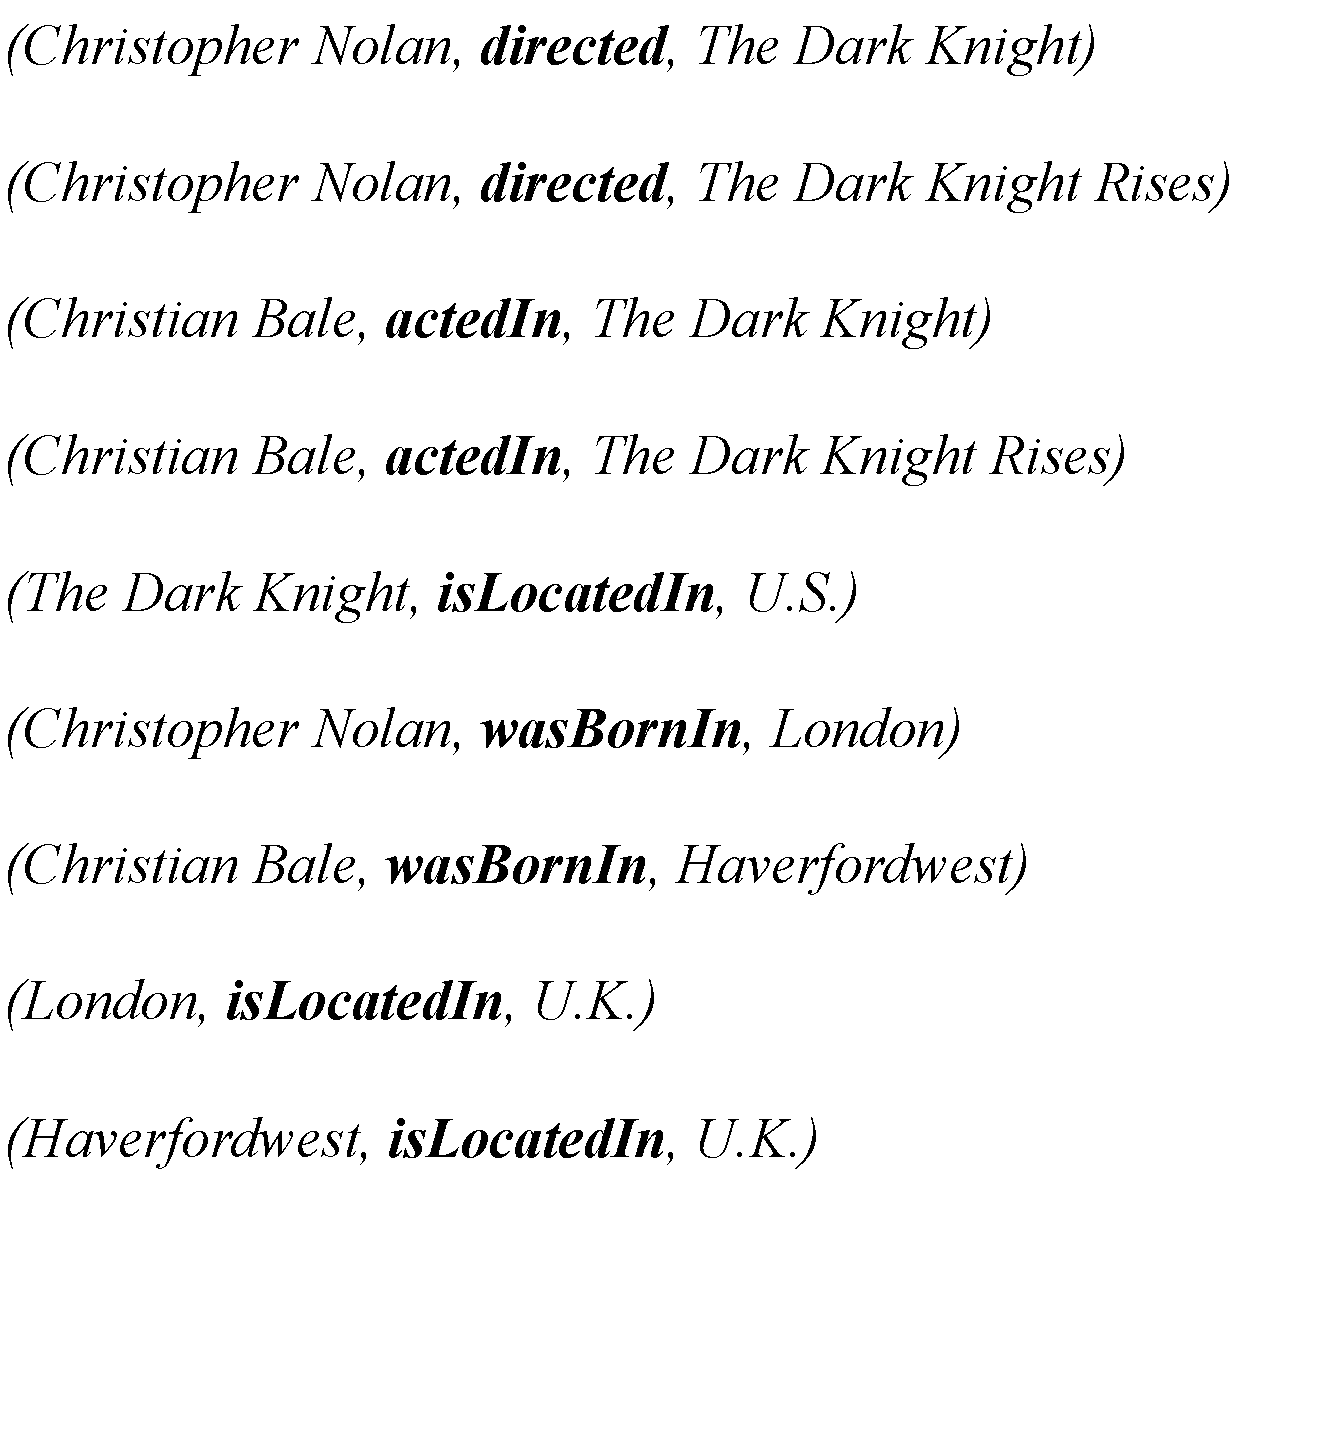
\includegraphics[width=0.3\textwidth]{2_KG_a.pdf}
    \label{2_KG_a}
  }
  \subfloat[有向图]{
    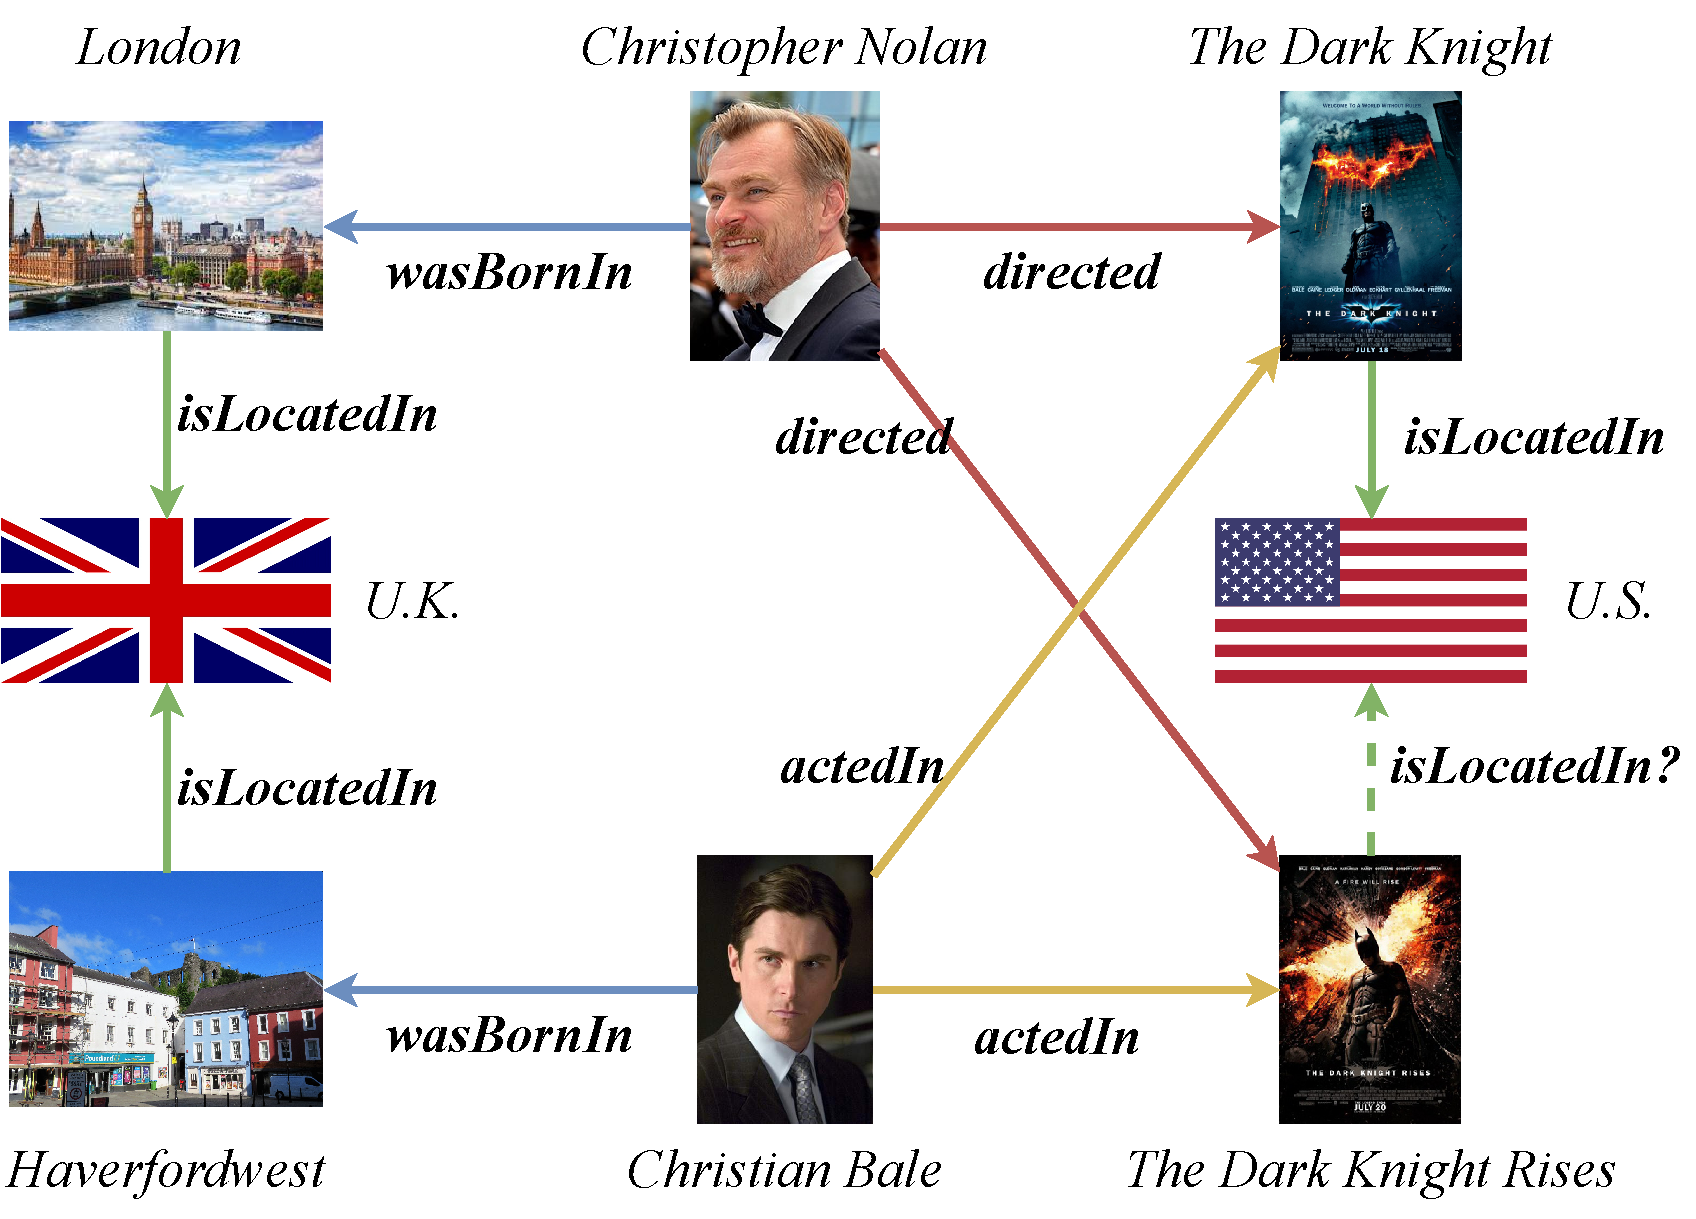
\includegraphics[width=0.6\textwidth]{2_KG_b.pdf}
    \label{2_KG_b}
  }
  \caption{知识图谱中的实体与关系}
  \label{2_KG}
\end{figure}

知识图谱能够有效地表示知识图谱中的结构化数据,但是难以被计算机进行直接处理和利用,需要先通过知识图谱表示学习的过程将知识转换为向量的形式,才能应用于各类知识图谱推理任务。
使用粗体字符表示知识图谱表示向量,则完成知识表示后的三元组为$\left(\bm{h}, \bm{r}, \bm{t}\right) \in \mathbb{R}^{\mathrm{d}}$,这里假定知识表示的向量空间为维度是$d$维的欧氏空间,根据模型的需要,也可以投影到其他类型的向量空间。
总的来说,知识图谱表示学习任务目的在于构建知识图谱表示学习模型,能够捕获知识图谱中的关键信息并将知识转换为向量形式,为下游任务提供数据支持。

通常情况下,知识图谱表示学习模型主要包含以下三个组成部分,分别是:
\begin{itemize}
  \item [1)] 知识表示空间。现有的研究工作中,表示空间包含点空间、流空间、复向量空间、高斯分布和离散空间等。
  \item [2)] 用于评估知识三元组合理性的评分函数。评分函数主要可以分为基于距离的和基于相似度匹配的评分函数。
  \item [3)] 用于学习将知识编码成向量形式的编码模型。编码模型是当前研究的重点内容,主要包括线性、双线性、矩阵分解和神经网络等多种类型。
\end{itemize}
此外,知识图谱表示学习模型还可以补充其他用于提高表示模型效果的辅助信息,包括文本、视觉和听觉等多种模态的相关信息。

知识图谱表示学习模型的构建过程主要包含以下三个步骤:
\begin{itemize}
  \item [1)] 定义知识在向量空间的表示形式。在这一步中,需要选择向量空间,设计编码模型,并确定是否需要辅助信息。
  \item [2)] 定义评分函数。评分函数可以表示为$f_r(h, t)$,用于评价知识$(h, r, t)$的合理性。一般而言,知识图谱中已知的事实知识三元组的得分会高于潜在事实三元组的得分。
  \item [3)] 学习知识表示,使知识图谱事实三元组的总置信度最大化。
\end{itemize}
通过上述步骤能够得到一个有效的知识图谱表示学习模型,该模型能够将知识表示为向量的形式,并能够用于各类知识图谱下游任务。

本章涉及到的相关符号及定义如表\ref{2_symbols}所示。
\begin{table}[ht]
  \centering
  \caption{本章符号定义}
  \begin{tabular*}{0.8\textwidth}{@{\extracolsep{\fill}}clcl}
		\toprule[1pt]
    符号 & 描述 & 符号 & 描述 \\ \hline
    $G$ & 知识图谱 & $F$ & 知识图谱事实集合\\
    $\mathbb{R}^{\mathrm{d}}$ & $d$维欧氏空间 & $h$ & 节点\\
    $\|\cdot\|_{p}$ & $p$范数 & $\alpha$ & 注意力权重\\
    $\circ$ & 哈达玛积运算 & $D$ & 数据集合\\
    $\bmod$ & 求余运算 & $\lambda$ & 权重\\ 
    $E(\cdot)$ & 期望计算 & $dim$ & 向量嵌入维度\\
    $\rho$ & 半径坐标 & $\gamma$ & 固定边界值\\
    $\theta$ & 角坐标 & $m$ & 消息\\
    $n$ & 邻域节点 & $L$ & 最大消息传递距离\\
		\bottomrule[1pt]
	\end{tabular*}
  \label{2_symbols}
\end{table}

\section{模型概览}
本章提出的NORMAN模型可以根据知识图谱的语义和结构信息,将实体和关系转换为表示向量。图\ref{2_NORMAN}展示了NORMAN模型的结构框架信息。
首先模型会对输入的知识图谱进行层次信息提取,该部分使用欧氏空间作为表示空间,采用基于距离的评分函数,并构建了基于极坐标系的编码模型,能够利用极坐标系的特性捕获知识图谱的层次信息,并将知识转化为表示向量。
随后采用图神经网络模型捕获知识图谱的邻域信息。在训练过程中将层次信息提取得到的向量通过一个全连接层进行映射得到初始向量,并通过邻域节点间的消息传递进行向量更新。
完成训练后的模型能够将输入的知识三元组转换为表示向量,并用于后续的知识推理任务。
\begin{figure}[H]
  \centering
  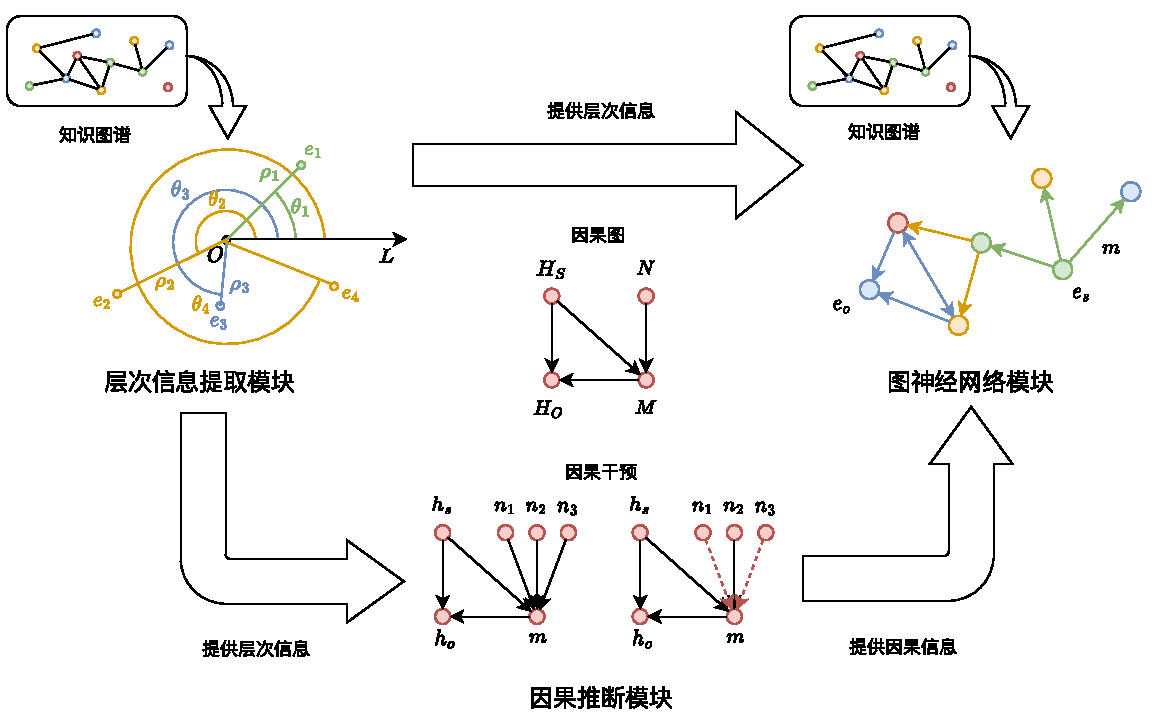
\includegraphics[width=1.0\textwidth]{2_NORMAN}
  \caption{基于图神经网络的知识图谱表示学习模型框架图}
  \label{2_NORMAN}
\end{figure}

\section{层次信息提取}
现有的知识图谱表示学习模型主要侧重于建模对称、反对称、逆向和组成等关系模式。然而,许多现有模型无法表示知识图谱中的层次信息,这限制了模型的表示能力。
为了应对这一挑战,NORMAN模型首先提出一种基于极坐标系的编码器对知识图谱进行编码,从而捕获知识图谱中的层次信息,并将获取到的知识向量作为输入提供给图神经网络模型。

层次信息在知识图谱中非常常见,以图\ref{1_KG}中展示的知识图谱为例,可以发现知识图谱中的实体与关系存在的层次信息可以表示为类似同心圆的层次结构,在该结构中靠近圆心的部分是层次级别较高的实体和关系,远离圆心的部分则对应层次级别较低的实体和关系。
同时,知识图谱中的实体和关系存在长尾分布的情况。以FB15K-237知识图谱为例,对知识图谱中出现次数最多的100个实体和关系对应的知识数量分别进行了统计,得到的知识数量分布情况如图\ref{2_LongTail}所示。可以发现知识图谱中的一小部分实体对应了大部分的知识数据,而大部分实体则只有很少的知识数据。关系的知识数量分布分布情况也同样呈现长尾分布情况。

因此,为了更好地捕获知识图谱中的层次信息,同时对不同类型的实体和关系进行区分,本文选择使用基于极坐标系的编码模型对知识图谱进行编码,这是因为极坐标系上任意一点的位置是根据其到极点的距离$\rho$(半径坐标)和其与极轴按照逆时针方向计算的角度$\theta$(角坐标)所唯一确定的。通过将知识图谱中层次级别较高的实体和关系映射到靠近极点(半径坐标模量较小)的位置,将层次较低的内容映射到远离极点(半径坐标模量较大)的位置,能够对知识图谱中的层次信息进行表示。同时,还可以通过调整实体和关系的角坐标实现对不同实体和关系的区分。上述思路在具体实现的过程中主要是通过模块的评分函数进行体现。
此外,在表示空间的选择方面,本文选择欧氏空间作为知识表示空间,主要是因为可以将极坐标系下的欧氏距离度量函数融入评分函数中,从而保证知识图谱表示学习过程的正确性。
\begin{figure}
  \centering
  \subfloat[实体的知识数量分布情况]{
    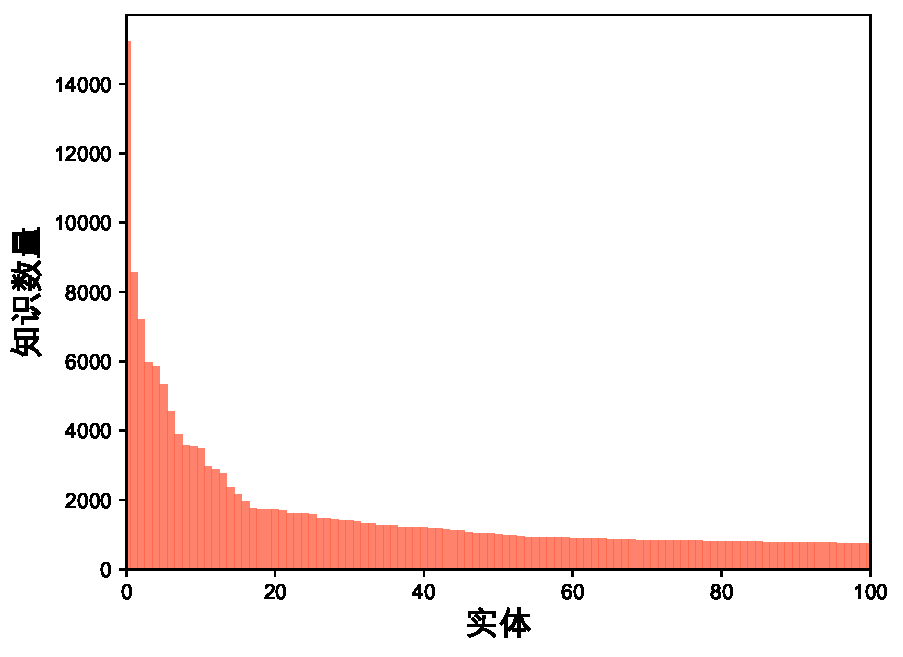
\includegraphics[width=0.45\textwidth]{2_LongTail_a.pdf}
    \label{2_LongTail_a}
  }
  \subfloat[关系的知识数量分布情况]{
    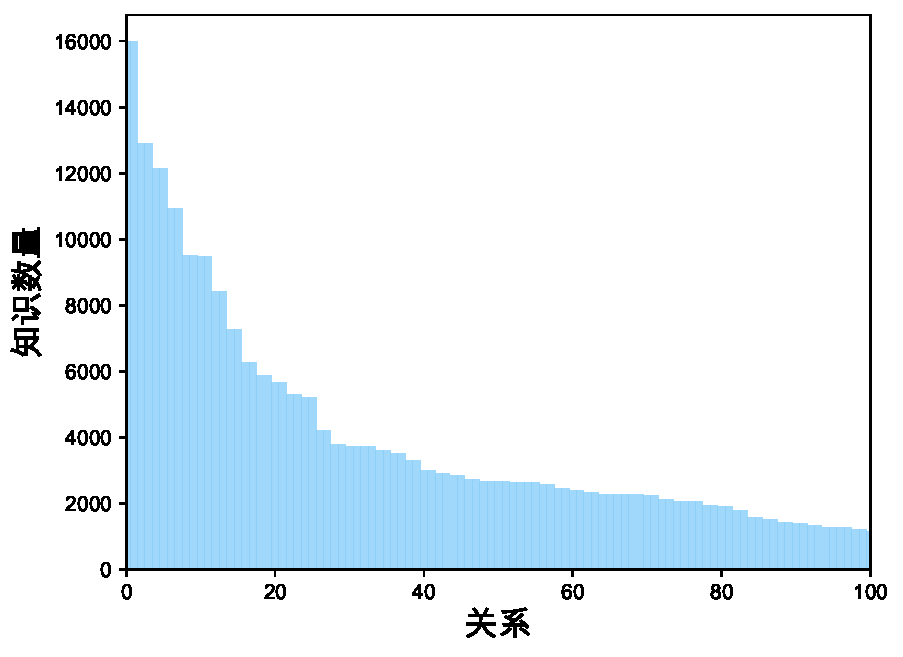
\includegraphics[width=0.45\textwidth]{2_LongTail_b.pdf}
    \label{2_LongTail_b}
  }
  \caption{FB15K-237知识图谱实体和关系的长尾分布情况}
  \label{2_LongTail}
\end{figure}

首先可以通过基于极坐标系的编码模型将知识图谱中的知识编码为欧氏空间的表示向量,在结果中,每个实体和关系都对应着一个极坐标,可以表示为$(\bm{\rho}, \bm{\theta})$,其中$\bm{\rho}$表示半径坐标向量,$\bm{\theta}$表示角坐标向量。同时半径坐标向量主要用于区分实体和关系的层次情况,而角坐标向量主要用于区分不同的实体和关系,从而保证了模块对知识图谱的表示能力。
在使用极坐标系编码器在欧氏空间上对知识图谱进行编码时,需要考虑如何设计得分函数的问题。本文计划采用基于距离的评分函数,考虑将极坐标系下的欧氏距离度量函数融入评分函数中,以保证知识图谱学习过程的正确性。
对此,需要先分析如何通过计算得到极坐标系上的两点之间欧氏距离。

对极坐标系上的两点$p$和$q$,可以将两点表示为向量形式$\bm{p}$和$\bm{q}$。设$p$和$q$的极坐标分别为$(\bm{\rho_1}, \bm{\theta_1})$和$(\bm{\rho_2}, \bm{\theta_2})$,则两点之间的欧氏距离可以具体表示为:
\begin{equation}
  \|\bm{p}-\bm{q}\|_2=\left(\bm{\rho_1}^2-2 \bm{\rho_1} \bm{\rho_2} \cos \left(\bm{\theta_1}-\bm{\theta_2}\right)+\bm{\rho_2}^2\right)^{\frac{1}{2}}
  \label{equation_distance}
\end{equation}

通过应用公式\ref{equation_distance},可以采用基于距离的得分函数,实现知识三元组$(h, r, t)$的评分。
设$h, r, t$的极坐标分别是$\left(\bm{\rho_1}, \bm{\theta_1}\right)$,$\left(\bm{\rho_2}, \bm{\theta_2}\right)$和$\left(\bm{\rho_3}, \bm{\theta_3}\right)$,同时当$(h, r, t) \in F$时设它们的表示向量有$\|\bm{h} + \bm{r} - \bm{t}\|_2 = 0$,根据该假设可以得到极坐标系下欧氏距离的得分函数$f^E_r(h, t)$为:
\begin{equation}
  \begin{aligned}
    f^{E}_{r}\left(h, t\right) & =-\left\|\bm{h}+\bm{r}-\bm{t}\right\|_2 \\
    & =-(\bm{\rho_1}^2+\bm{\rho_2}^2+\bm{\rho_3}^2 + 2 \bm{\rho_1} \bm{\rho_2} \cos \left(\bm{\theta_1}-\bm{\theta_2}\right) \\
    & - 2 \bm{\rho_1} \bm{\rho_3} \cos \left(\bm{\theta_1}-\bm{\theta_3}\right) - 2 \bm{\rho_2} \bm{\rho_3} \cos \left(\bm{\theta_2}-\bm{\theta_3}\right))^{\frac{1}{2}}
  \end{aligned}
\end{equation}
该评分函数的思想是,将关系$r$视为极坐标系上的点$h$到$t$的变换,即有$\bm{h} + \bm{r} = \bm{t}$,目标是使得正例三元组的评分尽可能接近为零,同时使负例三元组的得分尽量较高。

然而,仅使用基于距离的得分函数$f^E_r(h, t)$是不够的,原因是欧氏距离得分函数$f^E_r(h, t)$在实际训练过程中并没有具体区分半径坐标和角坐标,导致无法使用半径坐标来学习知识图谱中的层次信息,同时也没有使用角坐标来区分不同的实体和关系类别。
对此,模块针对半径坐标和角坐标分别设计了两种得分函数,从而充分利用极坐标系的半径坐标和角坐标的优势进行知识图谱表示。

针对半径坐标,模块将$r$视为$h$到$t$的半径坐标缩放变化过程,即有$\bm{\rho_1} \circ \bm{\rho_2} = \bm{\rho_3}$,其中$\circ$为哈达玛积运算,即对向量$\bm{a}, \bm{b} \in \mathbb{R}^{d}$,有$\left(\mathbf{a} \circ \mathbf{b}\right)_i = \mathbf{a}_i \cdot \mathbf{b}_i$。
根据上述设定,可以得到半径坐标的得分函数$f^{\rho}_r(h, t)$为:
\begin{equation}
  f^{\rho}_r\left(h, t\right) =-\left\|\bm{\rho_1} \circ \bm{\rho_2} - \bm{\rho_3}\right\|_2
\end{equation}

针对角坐标,模块将$r$视为$h$到$t$的角坐标变换过程,即有$(\bm{\theta_1} + \bm{\theta_2}) \bmod 2 \pi = \bm{\theta_3}$,因此角坐标的得分函数为:
\begin{equation}
  f^{\theta}_r\left(h, t\right) =-\left\|\left(\bm{\theta_1}+\bm{\theta_2}\right) \bmod 2 \pi - \bm{\theta_3}\right\|_1
\end{equation}

最终模块整体的得分函数$f_r(h, t)$是对上述三个得分函数的加权求和,表示如下:
\begin{equation}
  \begin{aligned}
    f_r\left(h, t\right) &= -\lambda_1 f^{E}_r(h, t) -\lambda_2 f^{\rho}_r(h, t) -\lambda_3 f^{\theta}_r(h, t) \\
    &= -\lambda_1 \left\|\bm{h} + \bm{r} - \bm{t}\right\|_2 \\
    &-\lambda_2 \left\|\bm{\rho_1} \circ \bm{\rho_2} - \bm{\rho_3}\right\|_2 \\
    &-\left\|\left(\bm{\theta_1}+\bm{\theta_2}\right) \bmod 2 \pi - \bm{\theta_3}\right\|_1
  \end{aligned}
  \label{f_1}
\end{equation}
其中$\lambda_1$、$\lambda_2$和$\lambda_3$分别表示欧氏距离得分函数$f^E_r(h, t)$、半径坐标得分函数$f^{\rho}_r(h, t)$和角坐标得分函数$f^{\theta}_r(h, t)$的权重超参数。

在模型训练的过程中,采用自对抗负采样(Self-adversarial Negative Sampling)损失函数~\cite{sun2018rotate},可以表示为:
\begin{equation}
  \begin{aligned}
  L= & -\log \operatorname{Sigmoid}\left(\gamma-f_r(h, t)\right) \\
  & -\sum_{i=1}^n p\left(h_i, r_i, t_i\right) \log \operatorname{Sigmoid}(f_{r_i}(h_i, t_i))
  \end{aligned}
  \label{loss_1}
\end{equation}
其中$\gamma$是合页损失的固定边界值超参数,需要根据知识图谱进行手动调整。
同时,随机负例的采样概率$p(h_i, r_i, t_i)$可以表示为:
\begin{equation}
  p(h_i, r_i, t_i)=\frac{\exp f_{r_i}(h_i, t_i))}{\sum_j \exp f_{r_j}(h_j, t_j)}
\end{equation}

通过上述得分函数和损失函数训练模型即可实现在保证模型学习正确性的情况下,利用半径坐标捕获知识图谱中的层次信息,同时利用角坐标区分不同的实体和关系。

% \section{图神经网络模型}
\section{基于图神经网络模型的知识图谱表示学习}
随后对NORMAN模型的图神经网络模型部分进行介绍,该部分为NORMAN模型的核心部分,如图\ref{2_NORMAN}所示。
在模型构建的过程中,主要包含以下步骤:
首先需要进行向量的初始化,通过层次信息提取获取到的表示向量进行一个全连接层映射并获取模型的初始向量,即可完成图神经网络模型的初始化。
随后需要进行邻域子图构建,通过选择知识中的一个实体作为起点,递归地向外扩展节点,直到达到最大距离时停止,即可实现邻域子图的构建。
随后进行消息传递,通过消息聚合函数将邻域子图中其他节点的信息聚合起来,并通过信息更新函数将新获取到的消息与当前节点的原有信息结合,实现节点信息更新。同时在消息传递的过程中,对于各个邻域节点的信息需要利用注意力机制进行评估,从而区分不同节点的消息贡献程度。
完成模型训练后得到的图神经网络模型可以将知识信息转换成表示向量,并能够应用于知识图谱补全和知识图谱问答等下游任务中。

\subsection{模型初始化}
首先需要进行图神经网络模型的初始化。为了保留层次信息提取部分获取到的层次信息,本文选择采用一个全连接层,将层次信息提取部分获取到的知识表示向量$\bm{h}_{layer}$映射为图神经网络模型的初始向量$\bm{h}_{GNN}$。映射过程可以表示为:
\begin{equation}
  \bm{h}_{GNN} = \mathbf{W} \cdot \bm{h}_{layer}
\end{equation}
其中$\mathbf{W}$是待学习的映射矩阵。完成向量映射后可以将获取到的向量$\bm{h}_{GNN}$提供给图神经网络模型,完成图神经网络模型的初始化,同时能够在图神经网络中保留知识图谱的层次信息,提高知识表示的效果。

\subsection{邻域子图构建}
在利用图神经网络模型进行知识图谱表示时,需要进行邻域子图构建。
本文采用的邻域子图构建算法如\ref{algorithm_simple}所示。
算法首先以知识三元组中的一个实体作为起点,随后采用递归的方式从最新的一层向外扩展节点,直到扩展达到到最大距离$L$,此时所有起点到终点的路径长度均为最大距离$L$。
\begin{algorithm}[tb]
	\caption{邻域子图构建算法}
	\label{algorithm_simple}
	\begin{algorithmic}[1]
  \Require 知识图谱事实集合$F$, 实体$e$, 最大距离$L$
  \Ensure 知识图谱邻域子图$G_{neighbor}$
  \State $F_{e}^{0} \leftarrow \varnothing$ // 初始化邻域知识集合
  \State $E_{e}^{0} \leftarrow \{e\}$ // 初始化邻域实体集合
  \For{$i \leftarrow 1$ to $L$}
  \State $F_{e}^{i} \leftarrow \{(h_i, r_i, t_i) \in F \mid h_i \in E_{e}^{i-1}\}$ // 获取第$i$层邻域知识
  \State $E_{e}^{i} \leftarrow \{t_i \mid (h_i, r_i, t_i) \in F_{e}^{i}\}$ // 获取第$i$层邻域实体
  \EndFor
  \State $G_{neighbor} \leftarrow F_{e}$ // 获取知识图谱邻域子图
  \State \Return $G_{neighbor}$
	\end{algorithmic}
\end{algorithm} 

为了避免保存知识图谱邻域子图对系统内存造成的压力,本文选择让算法可以在每次向外扩展节点时进行消息传递,从而不再需要在完成整个知识图谱邻域子图构建后再进行消息传递。
完整的算法包含消息传递过程,如算法\ref{algorithm_GNN}所示。

\subsection{消息传递}
在进行邻域子图构建时,模块可以通过消息传递机制进行节点邻域信息的获取和节点信息的更新。
消息传递过程主要包括两步:首先进行消息聚合获取邻域子图中所有节点的节点信息(包括节点自身的信息),并通过聚合函数进行聚合。
这里设置$\bm{h_s}$为初始表示向量,$\bm{h_o}$为更新后的表示向量,$\bm{n}$为邻域节点表示向量,则消息聚合过程可以表示为:
\begin{equation}
  \bm{m} = \operatorname{AGGREGATE}(\bm{h_s}, \bm{n})
\end{equation}
完成消息聚合后可以得到消息向量$\bm{m}$,随后即可进行节点信息更新。通过使用更新函数将来自邻域的消息和节点自身信息结合起来,从而实现节点信息的更新。节点信息更新可以表示为:
\begin{equation}
  \bm{h_o} = \operatorname{UPDATE}(\bm{h_s}, \bm{m})
\end{equation}
上述两步也可以合并到一起,得到的消息传递函数可以表示为:
\begin{equation}
  \bm{h_o} = \operatorname{UPDATE}(\bm{h_s}, \operatorname{AGGREGATE}(\bm{h_s}, \bm{n}))
  \label{equation_MessagePassing}
\end{equation}
因此,在设计消息传递函数的过程中,主要需要考虑如何设计消息聚合部分和节点信息更新部分的内容。

考虑到给定不同的知识三元组,得到的邻域子图可能相同,但用于推理的证据通常情况下是不同的。因此,为了从邻域子图中获取与给定的知识三元组相关的知识并提高搜集邻域知识过程的可解释性,需要在消息聚合部分使用注意力机制以评估不同邻域知识的重要性,并采用一个GRU层作为门控机制,减少GNN模型的限制并维护信息的长期传播。根据上述分析构建的消息传递函数可以表示为:
\begin{equation}
  \bm{h_o} = \operatorname{GRU}(\mathbf{W} \cdot (\bm{h_s} + \sum_{\bm{n_i} \in \bm{n}}{\bm{\alpha} \cdot \bm{n_i}}))
  \label{equation_newMessagePassing}
\end{equation}
其中$\mathbf{W}$表示训练参数,同时注意力权重$\bm{\alpha}$可以表示为:
\begin{equation}
  \bm{\alpha} = \operatorname{Sigmoid}(\mathbf{W}_1 \cdot \operatorname{ReLU}(\mathbf{W}_2 \cdot (\bm{h_s} \oplus \bm{h_q} \oplus \bm{n_i})))
  \label{equation_Alpha}
\end{equation}
其中$\bm{h_q}$是查询问题的关系对应的表示向量,$\oplus$是向量拼接运算。
在使用消息传递机制完成了节点信息更新后,节点的表示向量中即可融入了层次信息和邻域信息,从而可以进行知识表示。

随后为了训练模型,需要选择适合的得分函数。
考虑到此时各个节点的表示向量中已经包含了最大距离为$L$的邻域子图内的信息,因此构建的得分函数可以直接采用一个线性层计算最终得分。
这里让$\bm{h_o}$表示知识三元组$(h, r, ?)$、$(h, ?, t)$或$(?, r, t)$中缺失信息的表示向量,则得分函数可以表示为:
\begin{equation}
  f_{r}(h, t) = \mathbf{W} \cdot \bm{h_o}
  \label{equation_GNNScore}
\end{equation}
模块可以使用得分函数计算目标知识三元组的得分,并根据得分排名选择缺失信息对应的实体或关系。

\begin{algorithm}[t]
	\caption{图神经网络模型算法}  
	\label{algorithm_GNN}
	\begin{algorithmic}[1]
  \Require 知识图谱事实集合$F$, 知识三元组$(h, r, t)$, 最大距离$L$
  \Ensure 知识表示向量$(\bm{h}, \bm{r}, \bm{t})$
  \State $F_H \leftarrow \operatorname{GetHierarchy}(F)$ // 通过层次信息提取获取初始知识表示向量集合
  \For{$\{\bm{h}, \bm{r}, \bm{t}\} \in F_H$}
  \State $\bm{h_q} \leftarrow \bm{r}$ // 获取查询关系向量
  \For{$\bm{e} \in \{\bm{h}, \bm{t}\}$}
  \State $F_{e}^{0} \leftarrow \varnothing$ // 初始化邻域知识集合
  \State $E_{e}^{0} \leftarrow \{e\}$ // 初始化邻域实体集合
  \For{$i \leftarrow 1$ to $L$}
  \State $F_{e}^{i} \leftarrow \{(h_i, r_i, t_i) \in F \mid h_i \in E_{e}^{i-1}\}$ // 获取第$i$层邻域知识
  \State $E_{e}^{i} \leftarrow \{t_i \mid (h_i, r_i, t_i) \in F_{e}^{i}\}$ // 获取第$i$层邻域实体
  \State $\bm{\alpha} = \operatorname{GetAttention}(\bm{e}, \bm{h_q}, E_{e}^{i}, F_H)$ // 通过公式\ref{equation_Alpha}获取注意力权重
  \State $\bm{e} \leftarrow \operatorname{MessagePassing}(\bm{e}, \alpha, E_{e}^{i}, F_H)$ // 通过公式\ref{equation_newMessagePassing}进行消息传递
  \EndFor
  \EndFor
  \EndFor
  \State $(\bm{h}, \bm{r}, \bm{t}) \leftarrow F_H$ // 获取知识表示向量
  \State \Return $(\bm{h}, \bm{r}, \bm{t})$
	\end{algorithmic}
\end{algorithm} 

模型训练过程采用的损失函数与层次信息提取模块的损失函数\ref{loss_1}相同,同样为自对抗负采样(Self-adversarial Negative Sampling)损失函数,可以表示为:
\begin{equation}
  \begin{aligned}
  L= & -\log \operatorname{Sigmoid}\left(\gamma-f_r(h, t)\right) \\
  & -\sum_{i=1}^n p\left(h_i, r_i, t_i\right) \log \operatorname{Sigmoid}(f_{r_i}(h_i, t_i))
  \end{aligned}
\end{equation}
其中$\gamma$是合页损失的固定边界值超参数,需要根据知识图谱进行手动调整。
同时,随机负例的采样概率$p(h_i, r_i, t_i)$可以表示为:
\begin{equation}
  p(h_i, r_i, t_i)=\frac{\exp f_{r_i}(h_i, t_i))}{\sum_j \exp f_{r_j}(h_j, t_j)}
\end{equation}

至此,完成了对知识图谱表示学习模型NORMAN的图神经网络部分的全部介绍。
整个图神经网络模块的具体使用过程如算法\ref{algorithm_GNN}所示,可以发现该算法中融合了邻域子图构建算法\ref{algorithm_simple},并在获取邻域子图的同时进行了消息传递和节点信息更新。
完成训练的图神经网络模型融合了层次信息和邻域信息,能够将输入的知识转换为表示向量,并为知识图谱补全等下游任务提供数据支持。


\section{实验评估}
本节在多个开源数据集上开展实验,从而对NORMAN模型的性能进行综合评估。
NORMAN模型使用Python语言编写,Python版本为3.10.1,使用的深度学习框架为PyTorch,版本为1.13.1。
同时,本节所有实验都是在型号为AMAX G448-X3的服务器上完成的,服务器的具体参数包括:CPU型号为Xeon Sliver 4314,GPU型号为GeForce RTX 3090,系统内存为64G,系统硬盘为500G,操作系统版本为Ubuntu 22.04.1 LTS。

\subsection{实验概览}
知识图谱表示学习模型的目标是将实体和关系嵌入到低维向量空间中,同时保留原有知识图谱的结构信息和底层语义信息。
由于通常难以直接评价知识图谱表示学习模型的好坏,因此常用的方法是利用模型解决知识图谱下游任务来评估模型效果。本文使用知识图谱补全进行模型评估,即给定不完整的查询三元组,要求根据知识图谱中已有的事实预测查询三元组中缺失的内容。
知识图谱补全可以表示为补全查询三元组$\left(h, r, ?\right)$,$(h, ?, t)$或$\left(?, r, t\right)$的问题,其中$?$表示待补全的内容。
在测试过程中,对于测试数据集中的每个三元组$(h, r, t)$,首先将头部实体$h$、关系$r$或尾部实体$t$替换为每个候选答案以创建一组候选三元组,随后使用得分函数$f_r\left(h, t\right)$计算所有候选三元组的得分,并按照降序对候选三元组进行排序,最后根据结果评估模型执行知识图谱补全的效果。需要注意的是,知识图谱补全任务也可以认为是单跳知识推理任务,要求模型能够根据给定的查询三元组通过单步知识推理获取答案。
% 本文开展的实验遵循Bordes等人提出的实体链接实验设置~\cite{bordes2013translating},该设置中不会将任何知识图谱中存在的事实三元组纳入结果序列中,从而确保结果中的三元组都是新的三元组。
知识图谱补全中常用的评价指标包括平均排序MR(正确答案排名的平均值)、平均倒数排序MRR(正确答案排名倒数的平均值)以及Hits@K(正确答案在序列中排名位于前K的比例)等。
平均排序MR的计算方式是$\mathrm{MR}=\frac{1}{|\mathrm{S}|} \sum_{\mathrm{i}=1}^{|\mathrm{S}|} \mathrm{rank}_{\mathrm{i}}=\frac{1}{|\mathrm{S}|}\left(\mathrm{rank}_1+\mathrm{rank}_2+\cdots+\mathrm{rank}_{\mathrm{i}}\right)$,其中$|\mathrm{S}|$是结果三元组的数量,$\mathrm{rank}_{\mathrm{i}}$是第$i$个三元组在知识图谱补全结果序列中的排名,也就是正确三元组在预测三元组序列中的排名。由此可见,平均排序MR的结果越小代表模型效果越好。
平均倒数排序MRR与平均排序MR较为类似,区别在于平均倒数排序是对排序结果的倒数进行求和,计算方式为$\operatorname{MRR}=\frac{1}{|\mathrm{S}|} \sum_{\mathrm{i}=1}^{|\mathrm{S}|} \frac{1}{\mathrm{rank}_{\mathrm{i}}}=\frac{1}{|\mathrm{S}|}\left(\frac{1}{\mathrm{rank}_1}+\frac{1}{\mathrm{rank}_2}+\cdots+\frac{1}{\mathrm{rank}_{\mathrm{i}}}\right)$。可以发现,MRR和MR具有相同的作用,都能够用于评估模型的知识图谱补全效果,同时根据相关工作介绍~\cite{hoyt2022unified},MR在多个性能指标上比MRR的表现更差,一般情况下推荐使用MRR作为评价指标,而不推荐使用MR。因此,本文选择MRR评估模型效果。
Hits@K是指在知识图谱补全结果序列中正确答案排名小于$K$的三元组的平均占比,计算方式为$\mathrm{Hits@K}=\frac{1}{|\mathrm{S}|} \sum_{\mathrm{i}=1}^{|\mathrm{S}|} \mathbb{I}\left(\operatorname{rank}_{\mathrm{i}} \leq \mathrm{K}\right)$,其中$|S|$是三元组总数,$K$是目标排名范围,$\mathbb{I}\left(\cdot\right)$是指示函数,即若括号中的条件为真则其函数值为1,否则为0。一般情况下,取$K$为1、3和10。可以直观地发现,Hits@K的指标越大表明模型在知识图谱补全上的效果越好。
综上所述,本文选择平均倒数排序MRR和Hits@K作为评价指标,评估模型在知识图谱补全上的效果。

本节首先介绍了知识图谱表示学习模型的实验内容,随后介绍了任务的评价指标、数据集和具体的实验设置,并比较了本文提出的NORMAN模型和其他基线知识图谱表示学习模型在知识图谱补全上的效果,进而对NORMAN模型的优势和劣势进行客观评估。

\subsection{数据集}
\begin{table}[t]
  \centering
  \caption{知识图谱补全数据集统计信息}
  \begin{tabular*}{0.95\textwidth}{@{\extracolsep{\fill}}lccccc}
    \toprule[1pt]
    数据集 & 实体数量 & 关系数量 & 训练集数量 & 验证集数量 & 测试集数量 \\ \hline
    FB15K-237 & 14541 & 237 & 272115 & 17535 & 20466\\
    WN18RR & 40943 & 11 & 86835 & 3034 & 3134\\
    NELL-995 & 75492 & 200 & 138793 & 7710 & 7710\\
    \bottomrule[1pt]
	\end{tabular*}
  \label{Datasets1}
\end{table}
本文采用的数据集包括:FB15K-237~\cite{toutanova2015representing}、WN18RR~\cite{dettmers2018convolutional}和NELL-995~\cite{xiong2017deeppath}。上述三个数据集分别是从大规模知识图谱Freebase~\cite{bollacker2008freebase}、WordNet~\cite{glorot2010understanding}和NELL~\cite{carlson2010toward}采样得到的。
FB15K-237数据集在对Freebase知识图谱进行采样时删除了逆向关系,同时保留了其中的对称、反对称和组合关系。因此在FB15K-237数据集上的知识图谱补全主要考察模型对上述三种关系的表达能力。在数据数量上,FB15K-237包含14541种实体和237种关系,同时包含了310116条三元组数据,数据量较大,需要模型能够处理大规模知识图谱数据。
WN18RR与FB15K-237类似,也是在对WordNet知识图谱进行采样时删除了逆向关系并保留了对称、反对称和组合关系,因此也是主要考察模型对上述三种关系的表达能力。WN18RR包含40943种实体和11种关系,并提供了93003条三元组数据,可以发现WN18RR的实体种类非常多,同时三元组数量较少,意味着每种实体对应的三元组数量较少,这增加了训练模型的难度。
NELL-995是从大规模知识图谱NELL中采样得到的数据集,保留了数量排名在前200名的关系对应的三元组数据。与FB15K-237和WN18RR不同的是,NELL-995保留了逆向关系,原因是该数据集是可以用于评估多跳知识推理问题的数据集,为了进行双向推理保留了双向边,因此NELL-995除了对称、反对称和组合关系外,还可以考察模型对逆向关系的表达能力。在数据数量上,NELL-995包含75492种实体和200种关系,并提供了154213条三元组。可以发现,NELL-995提供了较多的数据,需要模型有处理大规模知识图谱的能力。
实验采用的三种知识图谱补全数据集的具体统计信息如表\ref{Datasets1}所示。根据上述分析可知,三种数据集具有不同的特点,能够用于客观评估知识图谱表示学习模型的表示效果。

\subsection{基线模型}
本文选择了一些表现较好的方法作为基线模型进行对比:
\begin{itemize}
  \item [1)]\textbf{TransE:}Bordes等~\cite{bordes2013translating}提出的TransE模型是最经典的翻译模型,通过基于距离的评分函数将关系作为头实体和尾实体间的翻译,并将翻译后的两个实体间的距离作为得分,从而获取三元组的合理性。
  \item [2)]\textbf{DistMult:}Yang等~\cite{yang2015embedding}提出的DistMult模型则属于语义匹配模型,采用张量捕获知识图谱结构,并通过将语义信息矩阵限制为对角矩阵保证了算法的时间复杂度较低和准确度较高。
  \item [3)]\textbf{ComplEx:}Trouillon等~\cite{trouillon2016complex}提出的ComplEx模型是对DistMult的一种扩展,通过使用复数嵌入能够建模不对称关系并实现效果提升。
  \item [4)]\textbf{RotatE:}Sun等~\cite{sun2018rotate}提出的RotatE模型是另一种代表性的语义匹配模型,将关系视作复数空间中头实体到尾实体的旋转,具有较好的知识图谱表示与知识推理能力。
  \item [5)]\textbf{CGI:}Feng等~\cite{feng2021should}提出的CGI模型是一种代表性的因果推断知识图谱表示学习模型,采用图卷积神经网络模型进行知识图谱表示学习,并通过对邻域信息进行因果推断评估是否接收邻域信息。
  \item [6)]\textbf{ConvE:}Dettmers等~\cite{dettmers2018convolutional}提出的ConvE模型是经典的卷积神经网络神经推理模型,能够通过二维卷积捕获实体间的特征交互信息并实现知识推理。
  \item [7)]\textbf{GraIL:}Teru等~\cite{teru2020inductive}提出的GraIL模型是一种采用图神经网络的知识推理模型,能够捕获邻域信息并实现知识图谱表示和知识推理。
\end{itemize}
其中,TransE、DistMult、ComplEx、RotatE和CGI均为知识图谱表示学习模型,能够用得分函数对所有候选答案的得分进行排序。ConvE和GraIL则为知识推理模型,能够通过单跳知识推理的方式计算候选答案的置信度,并对候选答案的置信度进行排序。因此两类模型均能够完成知识图谱补全任务。

\subsection{实验设置}
\begin{table}[t]
  \centering
  \caption{知识图谱补全实验超参数设置情况}
  \begin{tabular*}{0.95\textwidth}{@{\extracolsep{\fill}}lcccc}
    \toprule[1pt]
    \multirow{2}{*}{超参数名称} & \multirow{2}{*}{取值范围} & \multicolumn{3}{c}{最佳超参数}\\ 
      & & FB15K-237 & WN18RR & NELL-995 \\ \hline
    负采样大小 & $\{128, 256, 512, 1024\}$ & 1024 & 256 & 256 \\
    $dim_1$ & $\{128, 256, 512, 1024\}$ & 512 & 1024 & 512 \\
    $dim_2$ & $\{16, 32, 48, 64, 80\}$ & 16 & 64 & 48 \\
    $\alpha$ & $\{1e\text{-}3, 2e\text{-}4, 5e\text{-}5, 2e\text{-}5\}$ & $5e\text{-}5$ & $5e\text{-}5$ & $2e\text{-}4$ \\
    $\lambda_1$ & $\{0.1, 0.2, 0.5, 1, 2\}$ & 1 & 0.5 & 0.5 \\
    $\lambda_2$ & $\{0.1, 0.2, 0.5, 1, 2\}$ & 1 & 2 & 1 \\
    $\lambda_3$ & $\{0.1, 0.2, 0.5, 1, 2\}$ & 1 & 1 & 0.5 \\
    $\gamma_1$ & $\{3, 6, 9, 12, 24\}$ & 6 & 9 & 24 \\
    $\gamma_2$ & $\{3, 6, 9, 12, 24\}$ & 6 & 9 & 24 \\
    L & $\{1, 2, 3, 4, 5\}$ & 5 & 5 & 5 \\
    \bottomrule[1pt]
  \end{tabular*}
  \label{Hyperparameters1}
\end{table}
在实验过程中,本文对模型的超参数进行了调整,并最终形成了一系列最优超参数。
在层次信息提取部分,需要调整的超参数主要是层次信息提取嵌入维度$dim_1$、距离部分权重$\lambda_1$、半径坐标部分权重$\lambda_2$、角坐标部分权重$\lambda_3$和合页损失值$\gamma_1$,需要根据不同的知识图谱进行调整。
在图神经网络部分,需要调整的超参数则主要是图神经网络嵌入维度$dim_2$、消息传递的最大距离$L$和合页损失值$\gamma_2$,需要根据实验需要和不同的知识图谱进行调整。在不同数据集上进行调整时发现,在不考虑时间复杂度的情况下都是距离$L$越大知识图谱表示效果越好。
除了上述各个模块所需的超参数外,模型训练时还需要设置负采样大小和学习率$\alpha$等信息。
具体超参数设置情况如表\ref{Hyperparameters1}所示。

此外,模型的训练过程中采用提前终止法(Early-stop)防止模型陷入过拟合,在FB15K-237和NELL-995数据集中在80000步停止,在WN18RR数据集中在100000步停止。训练批次大小统一设定为256。

\subsection{实验结果与分析}
% 整体结果分析
\subsubsection{知识图谱补全实验}
\begin{table}[t]
  \centering
  \caption{FB15K-237数据集知识图谱补全实验结果}
  \begin{tabular*}{0.95\textwidth}{@{\extracolsep{\fill}}lcccc}
    \toprule[1pt]
    \multirow{2}{*}{模型} & \multicolumn{4}{c}{FB15K-237} \\
      & MRR & Hits@1 & Hits@3 & Hits@10 \\ \hline
    TransE & 29.4 & 24.8 & 40.1 & 46.5 \\
    DistMult & 24.1 & 15.5 & 26.3 & 41.9 \\
    ComplEx & 24.7 & 15.8 & 27.5 & 42.8 \\
    RotatE & 33.7 & 24.1 & 38.6  & 53.3 \\
    CGI & 30.2 & 22.6 & 29.5 & 45.3 \\
    ConvE & 32.5 & 23.7 & 34.7 & 50.1 \\
    GraIL & 27.9 & 20.5 & 29.2 & 42.9 \\
    NORMAN & \textbf{39.8} & \textbf{31.5} & \textbf{45.7} & \textbf{57.8} \\
    \bottomrule[1pt]
  \end{tabular*}
  \label{Experiment1_FB15K-237}
\end{table}

首先在FB15K-237知识图谱上应用上述模型进行知识图谱补全,其中在CGI模型中本文选择使用RoBERTa作为预训练模型。评价指标采用MRR和Hits@K,$K$值分别取1、3和10。最终得到实验结果如表\ref{Experiment1_FB15K-237}所示。可以发现,本文提出的NORMAN模型能够在FB15K-237知识图谱上取得优秀的效果,并在四种指标上均取得最好的效果,分别相较于ComplEx模型实现了$0.4\%$、$1.2\%$、$2.3\%$和$0.6\%$的改进。这说明了本文提出的模型能够较好的利用层次信息和邻域信息,在大规模知识图谱上实现高质量知识图谱表示。
可以发现在FB15K-237知识图谱上,知识图谱表示学习模型的效果通常优于知识推理模型,根据对FB15K-237数据集的分析~\cite{wan2021reasoning}可以了解到FB15K-237数据集的结构与WN18RR和NELL-995存在差别,在FB15K-237中一到多类型的推理路径的数量较多,即一个节点可能有大量出边到达其他节点,因此在FB15K-237上应用知识推理模型进行推理时,模型容易卡在一些具有大量出边的中间节点上,从而难以到达正确的答案节点。

\begin{table}[t]
  \centering
  \caption{WN18RR数据集知识图谱补全实验结果}
  \begin{tabular*}{0.95\textwidth}{@{\extracolsep{\fill}}lcccc}
    \toprule[1pt]
    \multirow{2}{*}{模型} & \multicolumn{4}{c}{WN18RR} \\
      & MRR & Hits@1 & Hits@3 & Hits@10 \\ \hline
    TransE & 22.6 & 28.9 & 46.4 & 50.4 \\
    DistMult & 43.3 & 39.0 & 44.1 & 49.5 \\
    ComplEx & 44.5 & 41.2 & 46.3 & 51.0 \\
    RotatE & 47.6 & 42.8 & 49.2 & 57.1 \\
    CGI & 44.2 & 39.6 & 46.5 & 55.2 \\
    ConvE & 43.2 & 40.5 & 44.1 & 52.4 \\
    GraIL & 43.7 & 42.5 & 48.6 & 56.5 \\
    NORMAN & \textbf{53.6} & \textbf{48.8} & \textbf{54.6} & \textbf{62.9} \\
    \bottomrule[1pt]
  \end{tabular*}
  \label{Experiment1_WN18RR}
\end{table}

在WN18RR知识图谱上开展的实验结果如表\ref{Experiment1_WN18RR}所示。根据结果可以发现,NORMAN模型在MRR、Hits@1、Hist@3和Hits@10四个指标上均取得了最好的效果,相比其他模型分别提高了$6.0\%$、$6.0\%$、$5.4\%$和$5.8\%$的提升,体现了NORMAN能够结合层次信息和邻域信息实现从少量数据中充足的信息进行知识图谱表示学习,因此NORMAN模型适合于表示这种实体种类多而每种数据相对较少的知识图谱。

\begin{table}[t]
  \centering
  \caption{NELL-995数据集知识图谱补全实验结果}
  \begin{tabular*}{0.95\textwidth}{@{\extracolsep{\fill}}lcccc}
    \toprule[1pt]
    \multirow{2}{*}{模型} & \multicolumn{4}{c}{NELL-995} \\
      & MRR & Hits@1 & Hits@3 & Hits@10 \\ \hline
    TransE & 45.6 & 51.4 & 67.8 & 75.1 \\
    DistMult & 68.0 & 61.0 & 73.3 & 79.5 \\
    ComplEx & 68.4 & 61.2 & 76.1 & 82.1 \\
    RotatE & 50.8 & 54.8 & 69.2 & 78.8 \\
    CGI & 55.2 & 57.9 & 71.1 & 76.2 \\
    ConvE & 46.2 & 52.3 & 58.1 & 71.2 \\
    GraIL & 49.6 & 54.3 & 61.4 & 73.2 \\
    NORMAN & \textbf{68.7} & \textbf{61.4} & \textbf{76.3} & \textbf{87.5} \\
    \bottomrule[1pt]
  \end{tabular*}
  \label{Experiment1_NELL-995}
\end{table}

在NELL-995知识图谱上进行的实体链接实验对应的结果如表\ref{Experiment1_NELL-995}所示。根据结果可以发现,NORMAN模型可以实现优秀的效果。尽管如此,仍然可以发现NORMAN与ComplEx模型表现较为接近。根据数据集分析可以发现NELL-995知识图谱包含了逆向关系,这恰好是ComplEx模型的强项,能够通过在复数空间的嵌入实现对逆向关系的高质量建模,而本文提出的NORMAN模型则没有针对逆向关系进行独立的建模表示。然而,由于NORMAN模型能够综合层次信息和邻域信息建模知识图谱,因此能够提高对逆向关系的表示效果,从而总体上表现与ComplEx模型相当。同时相较于其他模型,NORMAN取得了更好的效果,证明了NORMAN模型具有很好的知识表示能力。

% 任务类别实验
为了评估NORMAN模型对不同关系类别的知识图谱补全的实施效果,本文采用NELL-995数据集并选择其中12种特定关系的知识图谱补全任务作为分析对象,对各个模型的表现结果分析如表\ref{Experiment1_tasks1}和表\ref{Experiment1_tasks2}所示,表中的评价指标为MRR。可以发现,本文提出的NORMAN模型在与其他知识图谱表示学习模型进行比较时均取得了很好的效果。同时,可以发现NORMAN模型相比知识推理模型也有较大提升,能够实现平均$27.3\%$的提升。说明模型能够综合层次信息和邻域信息实现高质量的知识图谱表示,并能够在简单的单跳知识推理任务上超越其他现有的知识图谱表示学习模型和知识推理模型。
\begin{table}[t]
  \centering
  \caption{NELL-995数据集知识图谱表示学习模型特定任务实验结果}
  \begin{tabular*}{0.95\textwidth}{@{\extracolsep{\fill}}lcccccc}
    \toprule[1pt]
    \multirow{2}{*}{\small{任务名称}} & \multicolumn{6}{c}{\small{NELL-995}} \\
      & \small{TransE} & \small{DistMult} & \small{ComplEx} & \small{RotatE} & \small{CGI} & \small{NORMAN} \\ \hline
    \small{OrganizationHiredPerson} & 40.4 & 70.9 & 72.3 & 44.7 & 51.9 & \textbf{74.3} \\
    \small{WorksFor} & 22.3 & 55.5 & 62.4 & 28.4 & 44.5 & \textbf{65.4} \\
    \small{TeamPlaysInLeague} & 52.8 & \textbf{68.5} & 67.2 & 50.7 & 56.7 & 67.9 \\
    \small{AthletePlaysInLeague} & 40.5 & \textbf{68.3} & 65.3 & 48.2 & 52.4 & 66.4 \\
    \small{AthletePlaysSport} & 41.7 & 70.2 & 68.2 & 47.9 & 54.6 & \textbf{72.5} \\
    \small{OrganizationHeadquarteredInCity} & 50.6 & 74.5 & 70.9 & 55.2 & 57.1 & \textbf{75.1} \\
    \small{AthletePlaysForTeam} & 44.0 & 67.3 & 70.2 & 51.3 & 56.5 & \textbf{72.3} \\
    \small{PersonLeadsOrganization} & 24.9 & 64.5 & 63.1 & 36.5 & 42.3 & \textbf{66.5} \\
    \small{PersonBornInLocation} & 37.7 & 68.9 & 66.5 & 41.5 & 44.2 & \textbf{72.7} \\
    \small{AgentBelongsToOrganization} & 23.5 & 65.6 & 69.2 & 31.2 & 51.5 & \textbf{70.2} \\
    \small{AthleteHomeStadium} & 23.9 & 63.1 & 66.4 & 43.8 & 59.2 & \textbf{69.9} \\
    \small{TeamPlaysSport} & 46.5 & \textbf{74.4} & 69.3 & 52.3 & 56.4 & 74.8 \\
    \bottomrule[1pt]
  \end{tabular*}
  \label{Experiment1_tasks1}
\end{table}
% (74.3-72.3+65.4-62.4+67.9-68.5+66.4-68.3+72.5-70.2+75.1-74.5+72.3-70.2+66.5-64.5+72.7-68.9+70.2-69.2+69.9-66.4+73.8-74.4)/12
% (74.3-51.9+65.4-44.5+67.9-56.7+66.4-52.4+72.5-54.6+75.1-57.1+72.3-56.5+66.5-42.3+72.7-44.2+70.2-51.5+69.9-59.2+73.8-56.4)/12
% 45.6 46.2 49.6
\begin{table}[t]
  \centering
  \caption{NELL-995数据集知识推理模型特定任务实验结果}
  \begin{tabular*}{0.95\textwidth}{@{\extracolsep{\fill}}lccc}
    \toprule[1pt]
    \multirow{2}{*}{\small{任务名称}} & \multicolumn{3}{c}{\small{NELL-995}} \\
      & \small{ConvE} & \small{GraIL} & \small{NORMAN} \\ \hline
    \small{OrganizationHiredPerson} & 42.5 & 47.8 & \textbf{74.3} \\
    \small{WorksFor} & 30.7 & 36.2 & \textbf{65.4} \\
    \small{TeamPlaysInLeague} & 53.1 & 54.1 & \textbf{67.9} \\
    \small{AthletePlaysInLeague} & 44.2 & 48.3 & \textbf{66.4} \\
    \small{AthletePlaysSport} & 46.3 & 47.8 & \textbf{72.5} \\
    \small{OrganizationHeadquarteredInCity} & 48.9 & 50.3 & \textbf{75.1} \\
    \small{AthletePlaysForTeam} & 42.3 & 46.8 & \textbf{72.3} \\
    \small{PersonLeadsOrganization} & 28.2 & 30.2 & \textbf{66.5} \\
    \small{PersonBornInLocation} & 39.4 & 38.5 & \textbf{72.7} \\
    \small{AgentBelongsToOrganization} & 25.5 & 31.6 & \textbf{70.2} \\
    \small{AthleteHomestAdium} & 30.9 & 33.4 & \textbf{69.9} \\
    \small{TeamPlaysSport} & 48.6 & 53.9 & \textbf{73.8} \\
    \bottomrule[1pt]
  \end{tabular*}
  \label{Experiment1_tasks2}
\end{table}
% ((74.3-47.8)+(65.4-36.2)+(67.9-54.1)+(66.4-48.3)+(72.5-47.8)+(75.1-50.3)+(72.3-46.8)+(66.5-30.2)+(72.7-39.4)+(70.2-31.6)+(69.9-33.4)+(73.8-53.9))/12

% 消融实验
\subsubsection{消融实验}
\begin{table}[t]
  \centering
  \caption{消融实验结果}
  \begin{tabular*}{0.95\textwidth}{@{\extracolsep{\fill}}lcccc}
    \toprule[1pt]
    \multirow{2}{*}{模型} & \multicolumn{4}{c}{FB15K-237} \\
      & MRR & Hits@1 & Hits@3 & Hits@10 \\ \hline
    NORMAN(w/o HM) & 34.4 & 29.3 & 39.5 & 53.8 \\
    NORMAN(w/o GNN) & 32.6 & 25.0 & 36.1 & 51.2 \\
    NORMAN(w/o ATT) & 36.5 & 29.5 & 42.8 & 55.6 \\
    NORMAN & \textbf{39.8} & \textbf{31.5} & \textbf{45.7} & \textbf{57.8} \\
    \bottomrule[1pt]
  \end{tabular*}
  \label{Experiment1_ablation}
\end{table}
为了评估模型的各个模块效果,本文对NORMAN模型的各个模块开展了消融实验。
构建的消融实验模型包括:NORMAN(w/o HM)、NORMAN(w/o GNN)、NORMAN(w/o ATT)以及完整的NORMAN模型。
其中,NORMAN(w/o HM)模型去除了层次信息提取部分,仅由图神经网络模型实现知识图谱表示学习,这导致模型无法使用层次信息提取获取到的初始知识表示向量获取初始向量。对此,图神经网络模块使用随机初始化向量作为替代。
NORMAN(w/o GNN)模型则是去除了图神经网络部分,仅由层次信息提取部分获取知识图谱表示信息并执行测试任务。
NORMAN(w/o ATT)模型则是去除了图神经网络消息传递函数中的注意力机制,同时采用取平均数的方式作为替代,此时模型将认为任何邻域的消息具有相同的重要性。
表\ref{Experiment1_ablation}展示了消融实验的结果。可以发现三种消融模型的效果相对于NORMAN模型均出现了显著的下降,其中NORMAN(w/o ATT)的效果与NORMAN模型最接近,同时NORMAN(w/o GNN)的效果比NORMAN(w/o HM)更差。
上述实验结果说明,层次信息提取、图神经网络和图神经网络中的注意力机制对于NORMAN模型都很重要。其中图神经网络中的注意力机制能够为不同的邻域节点提供相应的注意力权重,从而能够区分不同节点消息的重要性。
层次信息提取部分能够捕获知识的层次信息,同时为图神经网络模块提供初始向量,从而间接影响了图神经网络模块。
而图神经网络是模型的核心,首先通过采用层次信息提取部分获取的向量进行初始化,从而完成了知识图谱中层次信息的获取。随后模型通过构建邻域子图和进行消息传递,实现了邻域信息的捕获,从而提高了模型的知识表示效果。
因此,通过上述分析可以为模型各个部分的重要程度进行排序,即图神经网络部分最重要,其次是层次信息提取部分,最后是图神经网络中的注意力机制部分。

% 消息范围效果
\subsubsection{消息传递范围分析}
\begin{figure}[t]
  \centering
  \subfloat[FB15K-237数据集] {
    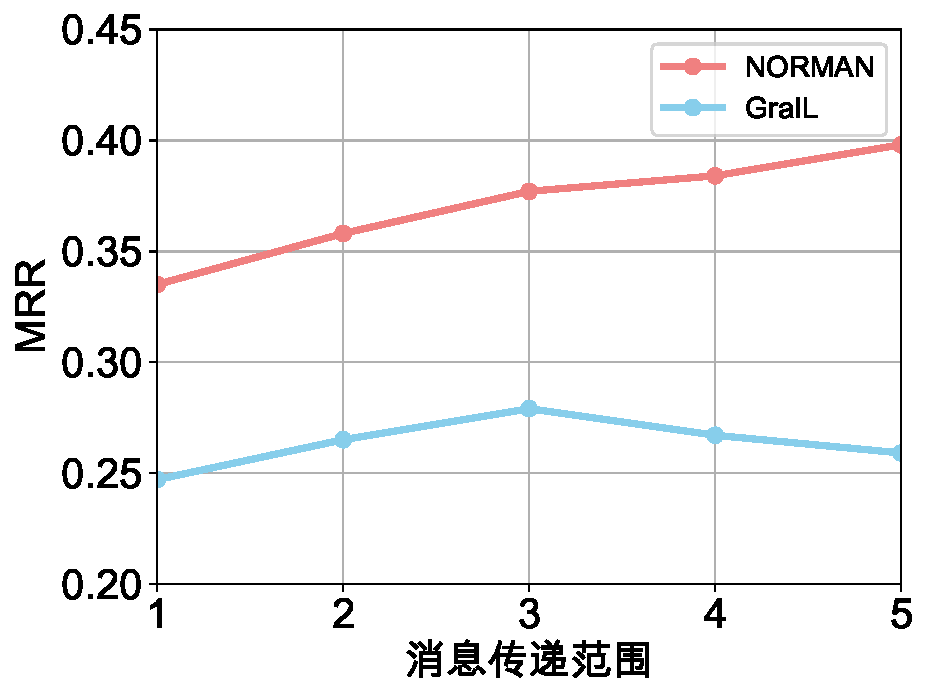
\includegraphics[width=0.3\textwidth]{2_NORMAN_messageRange_FB15K237.pdf}
    \label{Experiment1_messageRange_a}
  }
  \subfloat[WN18RR数据集] {
    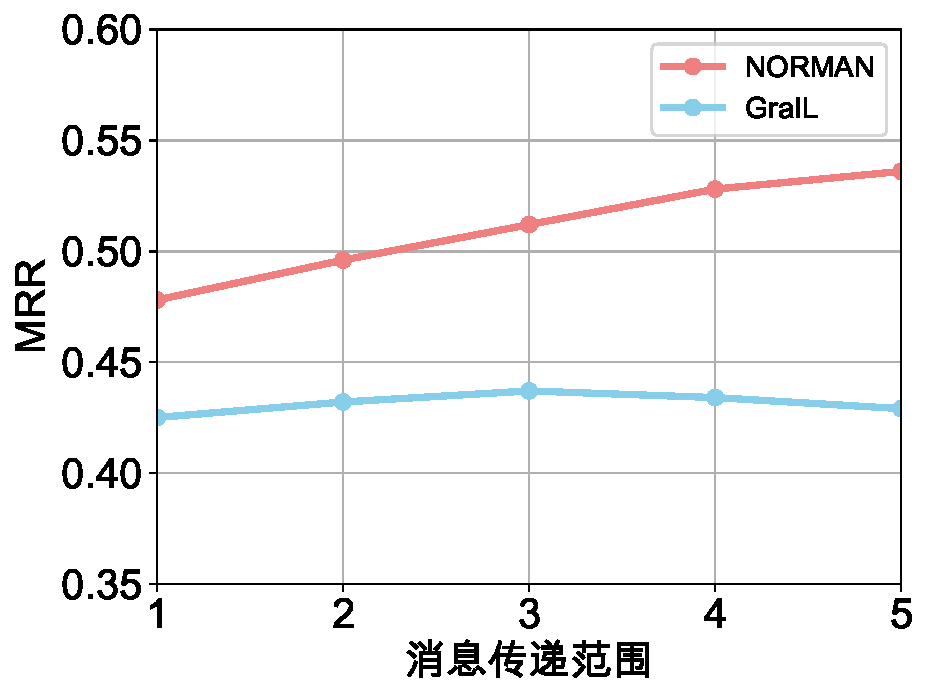
\includegraphics[width=0.3\textwidth]{2_NORMAN_messageRange_WN18RR.pdf}
    \label{Experiment1_messageRange_b}
  }
  \subfloat[NELL-995数据集] {
    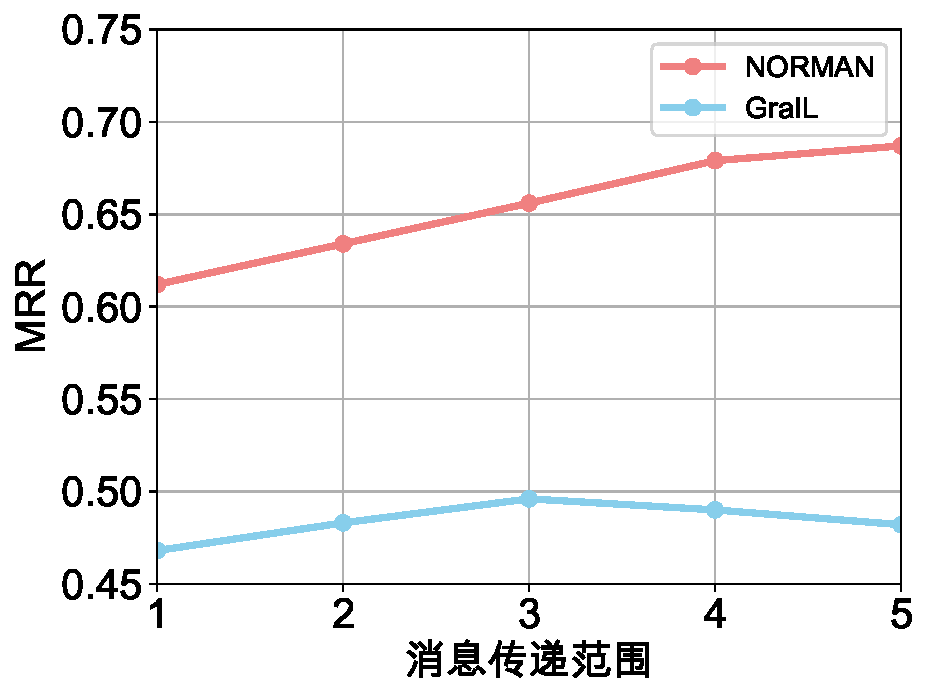
\includegraphics[width=0.3\textwidth]{2_NORMAN_messageRange_NELL995.pdf}
    \label{Experiment1_messageRange_c}
  }
  \caption{模型消息传递范围分析实验结果}
  \label{Experiment1_messageRange}
\end{figure}
为了更好地分析模型的图神经网络模块受到邻域消息范围$L$的影响,本文对$L$进行了调整,并统计了NORMAN模型在三种数据集上的表现,评价指标采用MRR。
同时本文选择同样采用图神经网络和消息传递机制的GraIL模型开展了对比实验。实验结果如图\ref{Experiment1_messageRange}所示。
可以发现,当设置$L$的范围为1到5时,随着邻域消息范围$L$的增长,本文提出的NORMAN模型在三种数据集上均能够实现效果的提升。这体现了模型采用的图神经网络模型具有较好的复杂知识表示能力,原因是模型能够在构建邻域子图的同时进行消息传递,实现节点信息的更新,从而保障了模型在邻域消息范围扩大的时候依然能够有效地实现知识表示。同时这也说明NORMAN模型采用注意力机制后能够对不同的邻域消息提供不同的权重,降低无关的和误导性的知识造成的影响,从而使得模型能够利用大范围的邻域信息进行知识图谱表示。
相比之下可以发现,GraIL模型的效果在$L$为3时达到最佳,当$L$继续增长时GraIL的效果将会出现下降。这说明了GraIL模型的图神经网络机制相比于NORMAN模型不能够有效地表示复杂结构的知识信息,从而导致了邻域子图范围超过3时模型效果出现下降。同时说明GraIL模型只能够有效利用范围较小的邻域信息,当邻域范围太大时,模型会因为无法对消息进行有效的筛选而受到干扰信息的影响,从而降低知识图谱表示效果。

% 可视化实验
\subsubsection{节点可视化分析}
\begin{figure}[t]
  \centering
  \subfloat[RotatE可视化结果]{
    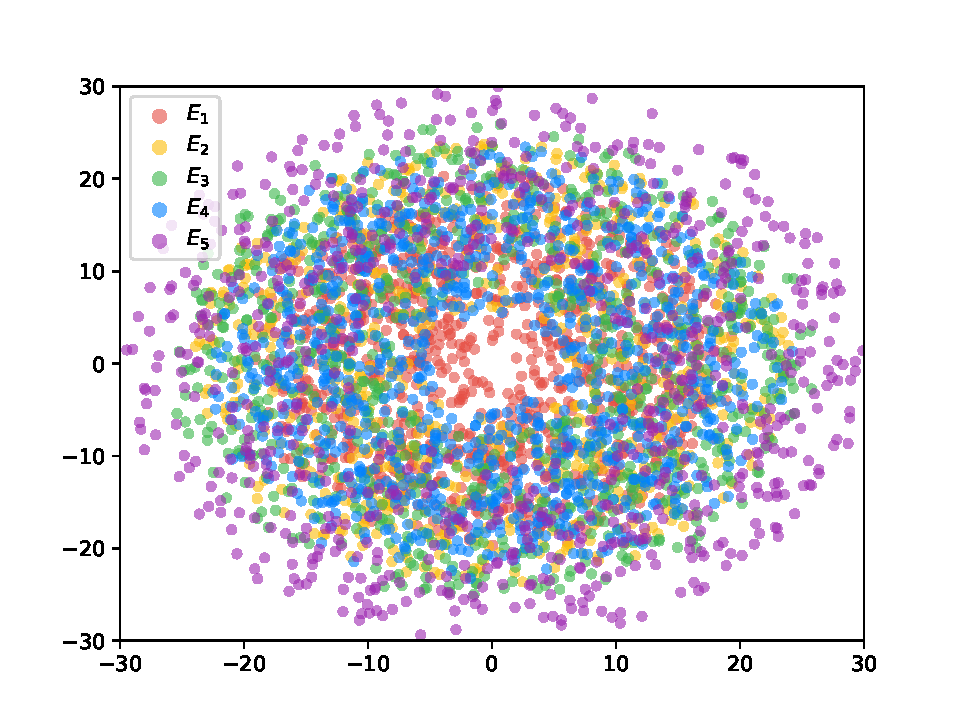
\includegraphics[width=0.4\textwidth]{2_RotatE_view.pdf}
    \label{Experiment1_figures_a}
  }
  \subfloat[NORMAN可视化结果]{
    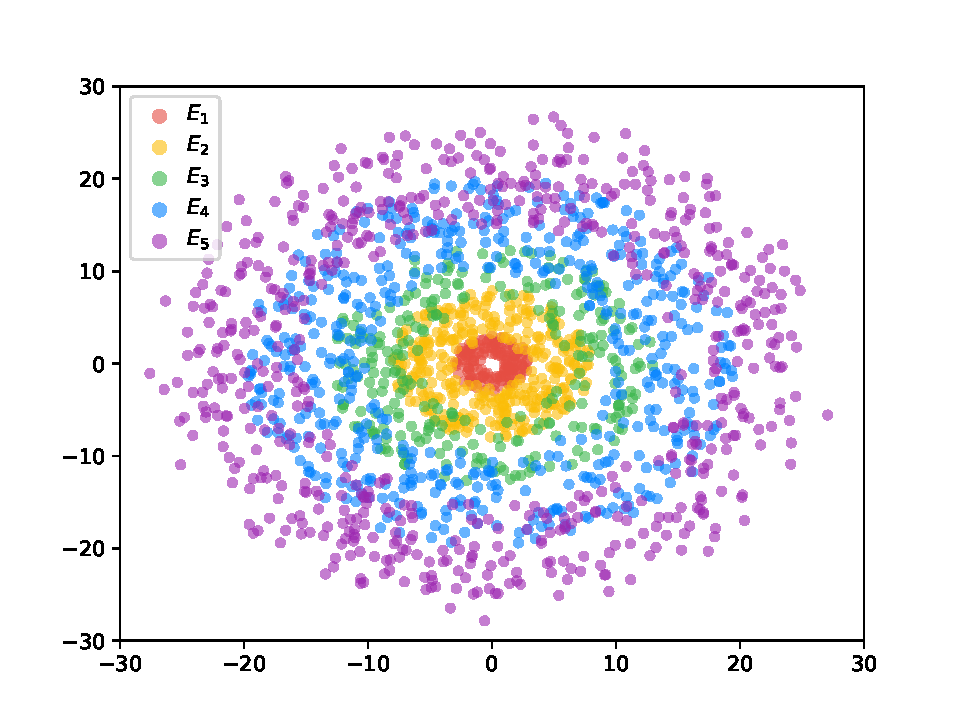
\includegraphics[width=0.4\textwidth]{2_NORMAN_view.pdf}
    \label{Experiment1_figures_b}
  }
  \caption{FB15K-237数据集部分节点可视化分析实验结果}
  \label{Experiment1_figures}
\end{figure}
为了更直观地分析模型对知识图谱层次信息的表示效果,本文将RotatE模型和NORMAN模型对FB15K-237知识图谱的部分节点在欧氏空间中的表示向量进行了可视化展示,其中不同的节点采用不同颜色的点进行表示,得到的结果如图\ref{Experiment1_figures}所示。
可以发现,RotatE模型得到的知识图谱表示向量分布较为均匀,不能对不同层次的实体进行区分。
这种情况主要是因为RotatE模型采用的基于旋转的复数空间表示方法没有对知识图谱内的层次信息进行建模,因而不能够很好地体现知识图谱中的层次信息。
NORMAN模型得到的知识图谱表示向量则能够清晰地将不同层次的实体进行区分,可以看到图中不同的实体之间存在明显的层次划分。
这主要是因为NORMAN模型的极坐标系编码器采用半径坐标对实体的层次级别进行表示,能够根据知识图谱中的层次信息为实体分配对应的半径坐标向量。
通过这种方法,NORMAN模型能够很好地捕获知识图谱中的层次信息,从而为知识图谱补全等下游任务提供支持,同时也能为本文提出的知识推理模型提供层次信息。

\section{本章小结}
本章主要介绍了基于图神经网络的知识图谱表示学习模型NORMAN。
NORMAN模型首先采用了一种基于极坐标系的编码器。该编码器能够将知识编码为极坐标向量的形式,其中半径坐标向量用于捕获知识的层次信息,角坐标向量则用于区分不同类别的知识。
随后模型采用了一种图神经网络模型。该模型首先利用层次信息提取过程得到的向量进行一个全连接层映射获取初始向量,随后通过递归方式实现邻域子图构建和消息传递,并通过消息聚合函数将邻域子图中的消息聚合起来,通过信息更新函数将消息与节点向量相结合,实现节点信息更新。同时在消息传递过程中,对各个邻域节点的消息采用注意力机制,从而区分不同节点的消息贡献程度。
本章首先给出了知识图谱表示学习任务的定义,随后给出了方法概览,并详细介绍了本文提出的基于图神经网络的知识图谱表示学习模型与策略,最后在公开数据集上进行了实验,验证了模型的效果。


\chapter{基于双重智能体强化学习的知识推理模型}
本章提出一种基于双重智能体强化学习的知识推理模型LAURA,构建了两种能够相互协作进行知识推理的强化学习智能体,能够根据知识图谱中的实体和层次信息进行知识推理,并通过协作动作空间、协作策略网络和协作奖励等方式实现信息交流和协作,共同实现高质量知识推理。
本章包含六个部分:知识推理任务定义(3.1节),模型概览(3.2节),强化学习框架(3.3节),双重智能体知识推理(3.4节),实验评估(3.5节),以及本章小结(3.6节)。

\section{知识推理任务定义}
知识推理任务可以表示为给定知识推理问题$Q$,其中包含了查询三元组$(h, r, ?)$、$(h, ?, t)$或$(?, r, t)$,目标是通过利用知识图谱上的知识集合$F$推理查询三元组中缺失的内容,并得到知识推理路径$p$。
需要注意的是$p$可以表示为由单个或多个知识组成的路径,例如给定问题$Q$的查询三元组为$(h, r, ?)$,则一条可行的知识推理路径可以表示为$p=\{(h, r, e_1), (e_1, r_1, e_2), \cdots, (e_{n-1}, r_{n-1}, t)\}$,可以理解为知识推理路径是首尾相连的多跳知识组成的集合,同时也可以简写为$p=h\xrightarrow{r}e_1\xrightarrow{r_1}e_2 \cdots e_{n-1}\xrightarrow{r_{n-1}}t$。

本章研究的问题是推理实体和关系的知识推理问题,并要求模型提供知识推理路径。
例如,以“现任美国总统乔·拜登居住在哪个城市”作为推理问题,则该问题对应的查询三元组为$(Joe Biden, livesInCity, ?)$,随后即可进行知识图谱查询。
如果知识图谱中不存在查询的知识,则需要由知识推理模型进行如图\ref{3_Task}所示的推理。
\begin{figure}[ht]
  \centering
  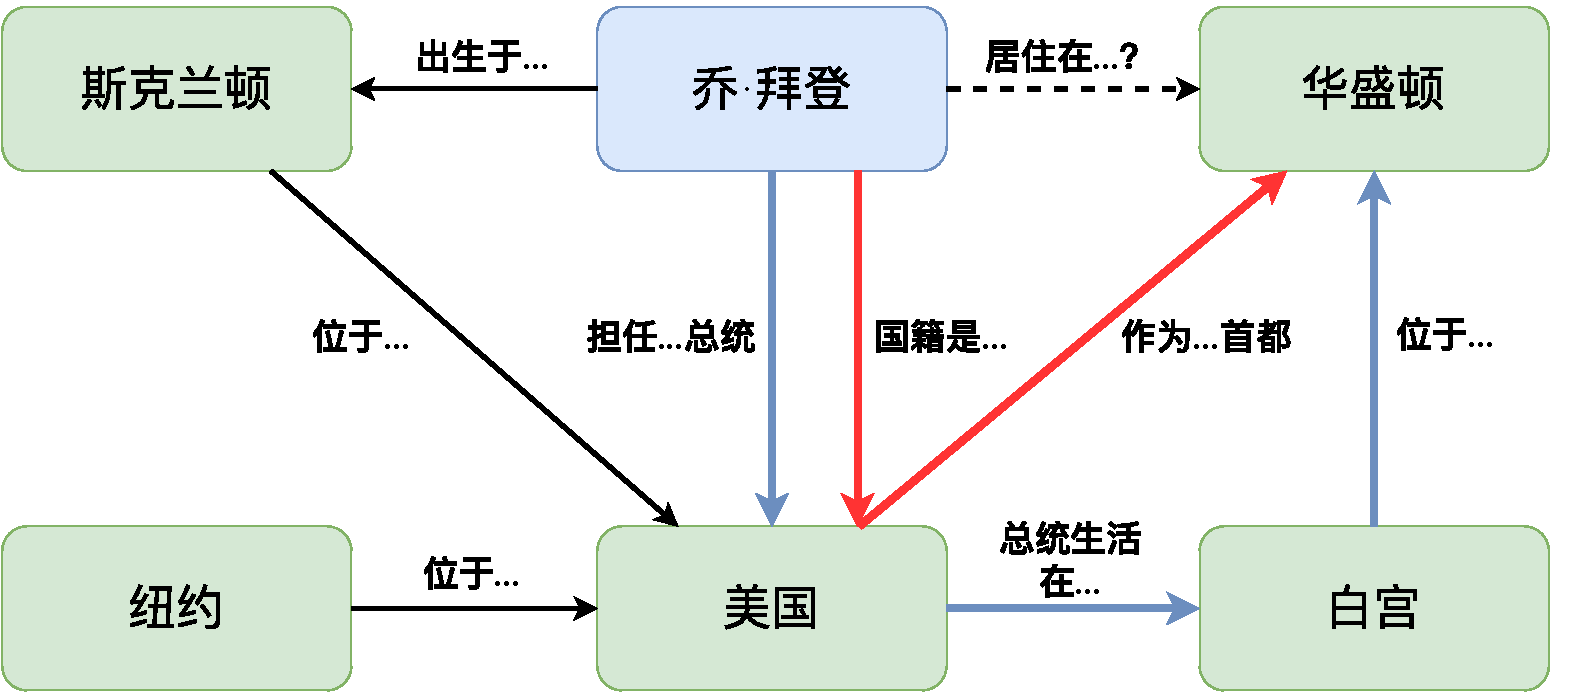
\includegraphics[width=0.8\textwidth]{3_Task}
  \caption{知识推理充分性示例}
  \label{3_Task}
\end{figure}

可以发现一条能够到达正确答案的推理路径如图中蓝色实线所示,可以表示为“拜登$\xrightarrow{\mbox{担任总统}}$美国$\xrightarrow{\mbox{总统生活在}}$白宫$\xrightarrow{\mbox{位于}}$华盛顿”。
同时可以发现另一条能够到达正确答案的推理路径如图中红色实线所示,可以表示为“拜登$\xrightarrow{\mbox{国籍}}$美国$\xrightarrow{\mbox{首都}}$华盛顿”。
这条路径虽然也能到达正确答案,但是这种推理是不充分的,因为并不是所有美国人都居住在首都华盛顿。
继续对这条推理路径进行分析,可以发现模型推理时使用了较高层次的知识(拜登是美国人),而利用较高层次的知识会导致候选答案变多,例如美国人可以生活在纽约、华盛顿和斯克兰顿等城市。
因此,如果希望模型能够正确推理,就需要模型能够正确利用不同层次的知识,实现候选答案的增加或减少,从而保证模型能够获取到正确答案。
本文提出的LAURA模型的一个重要动机是希望能够利用知识图谱中的层次信息增加知识推理路径的充分性,考虑到通常难以直接从知识图谱中获取明显的层次信息,因此模型利用了第二章的NORMAN模型实现知识图谱中层次信息的获取。

本章涉及到的符号及定义如表\ref{3_symbols}所示。
\begin{table}[ht]
  \centering
  \caption{本章符号定义}
  \begin{tabular*}{0.8\textwidth}{@{\extracolsep{\fill}}clcl}
		\toprule[1pt]
    符号 & 描述 & 符号 & 描述\\ \hline
    $G$ & 知识图谱 & $F$ & 知识图谱事实集合\\
    $e$ & 实体变量 & $h$ & 聚类节点变量\\
    $r$ & 关系变量 & $his$ & 历史信息变量\\
    $S$ & 状态信息 & $A$ & 动作空间\\
    $A^{add}$ & 额外动作空间 & $A^{co}$ & 协作动作空间\\
    $\pi_\theta$ & 策略网络 & $\operatorname{Similarity}(\cdot)$ & 相似度计算函数\\
    $\pi_\theta^{co}$ & 协作策略网络 & $\operatorname{Top@T}(\cdot)$ & 保留最高得分三元组函数\\
    $R$ & 奖励函数 & $\operatorname{Entity}(\cdot)$ & 获取聚类节点内实体函数\\
    $\hat{R}$ & 协作奖励 & $\operatorname{Hierarchy}(\cdot)$ & 获取实体对应聚类节点函数\\
    $p$ & 知识推理路径 & &\\
		\bottomrule[1pt]
	\end{tabular*}
  \label{3_symbols}
\end{table}

\section{模型概览}
本章提出的LAURA模型能够结合知识图谱表示学习模型NORMAN,通过强化学习框架实现多粒度的知识推理。
图\ref{3_LAURA}展示了该模型,可以发现模型包含了两个部分,分别是小型智能体知识推理和大型智能体知识推理。
两个部分均采用了强化学习框架,在知识图谱上由一个智能体(agent)根据策略网络(policy network)选取动作空间中的动作(action)并改变自身状态(state),当到达结束条件时根据任务完成情况得到对应的奖励(reward)。
两种智能体均能够独立进行知识推理,它们主要区别在于:大型智能体利用NORMAN模型获取知识图谱中的实体和关系的层次信息,并通过聚类的方式将层次级别相近的实体构建为聚类节点,根据聚类节点间是否有知识关联构建聚类边,从而完成了聚类知识图谱的构建。在知识推理过程中,大型智能体在聚类知识图谱上进行知识推理,而小型智能体则是在原始知识图谱上进行知识推理。
为了实现两种智能体之间的信息交流,模型还包含了协作动作空间、协作策略网络和协作奖励。
进行知识推理时协作动作空间能够保证两个智能体的动作空间相互覆盖,协作策略网络能够保证两个智能体能够交流对方的历史状态,协作奖励能够鼓励两个智能体沿着相似的推理路径前进并帮助另一个智能体达到正确目标。
利用模型进行知识推理的过程可以简单描述为:首先由大型智能体进行一次单跳知识推理,随后由小型智能体进行一次单跳知识推理,在推理过程中两种智能体可以通过协作动作空间、协作策略网络和协作奖励进行信息交流和轨迹协调,重复上述步骤,直到两种智能体分别到达各自的推理距离上限时停止协作推理过程,并返回置信度最高的知识推理路径作为推理结果。
需要注意的是,LAURA模型在开始知识推理前首先在两种知识图谱的每个节点上添加了自环和反向边,从而使得智能体能够在知识图谱上进行双向推理和提前停止在某个节点上。

\begin{figure}
  \centering
  \subfloat[小型智能体知识推理] {
    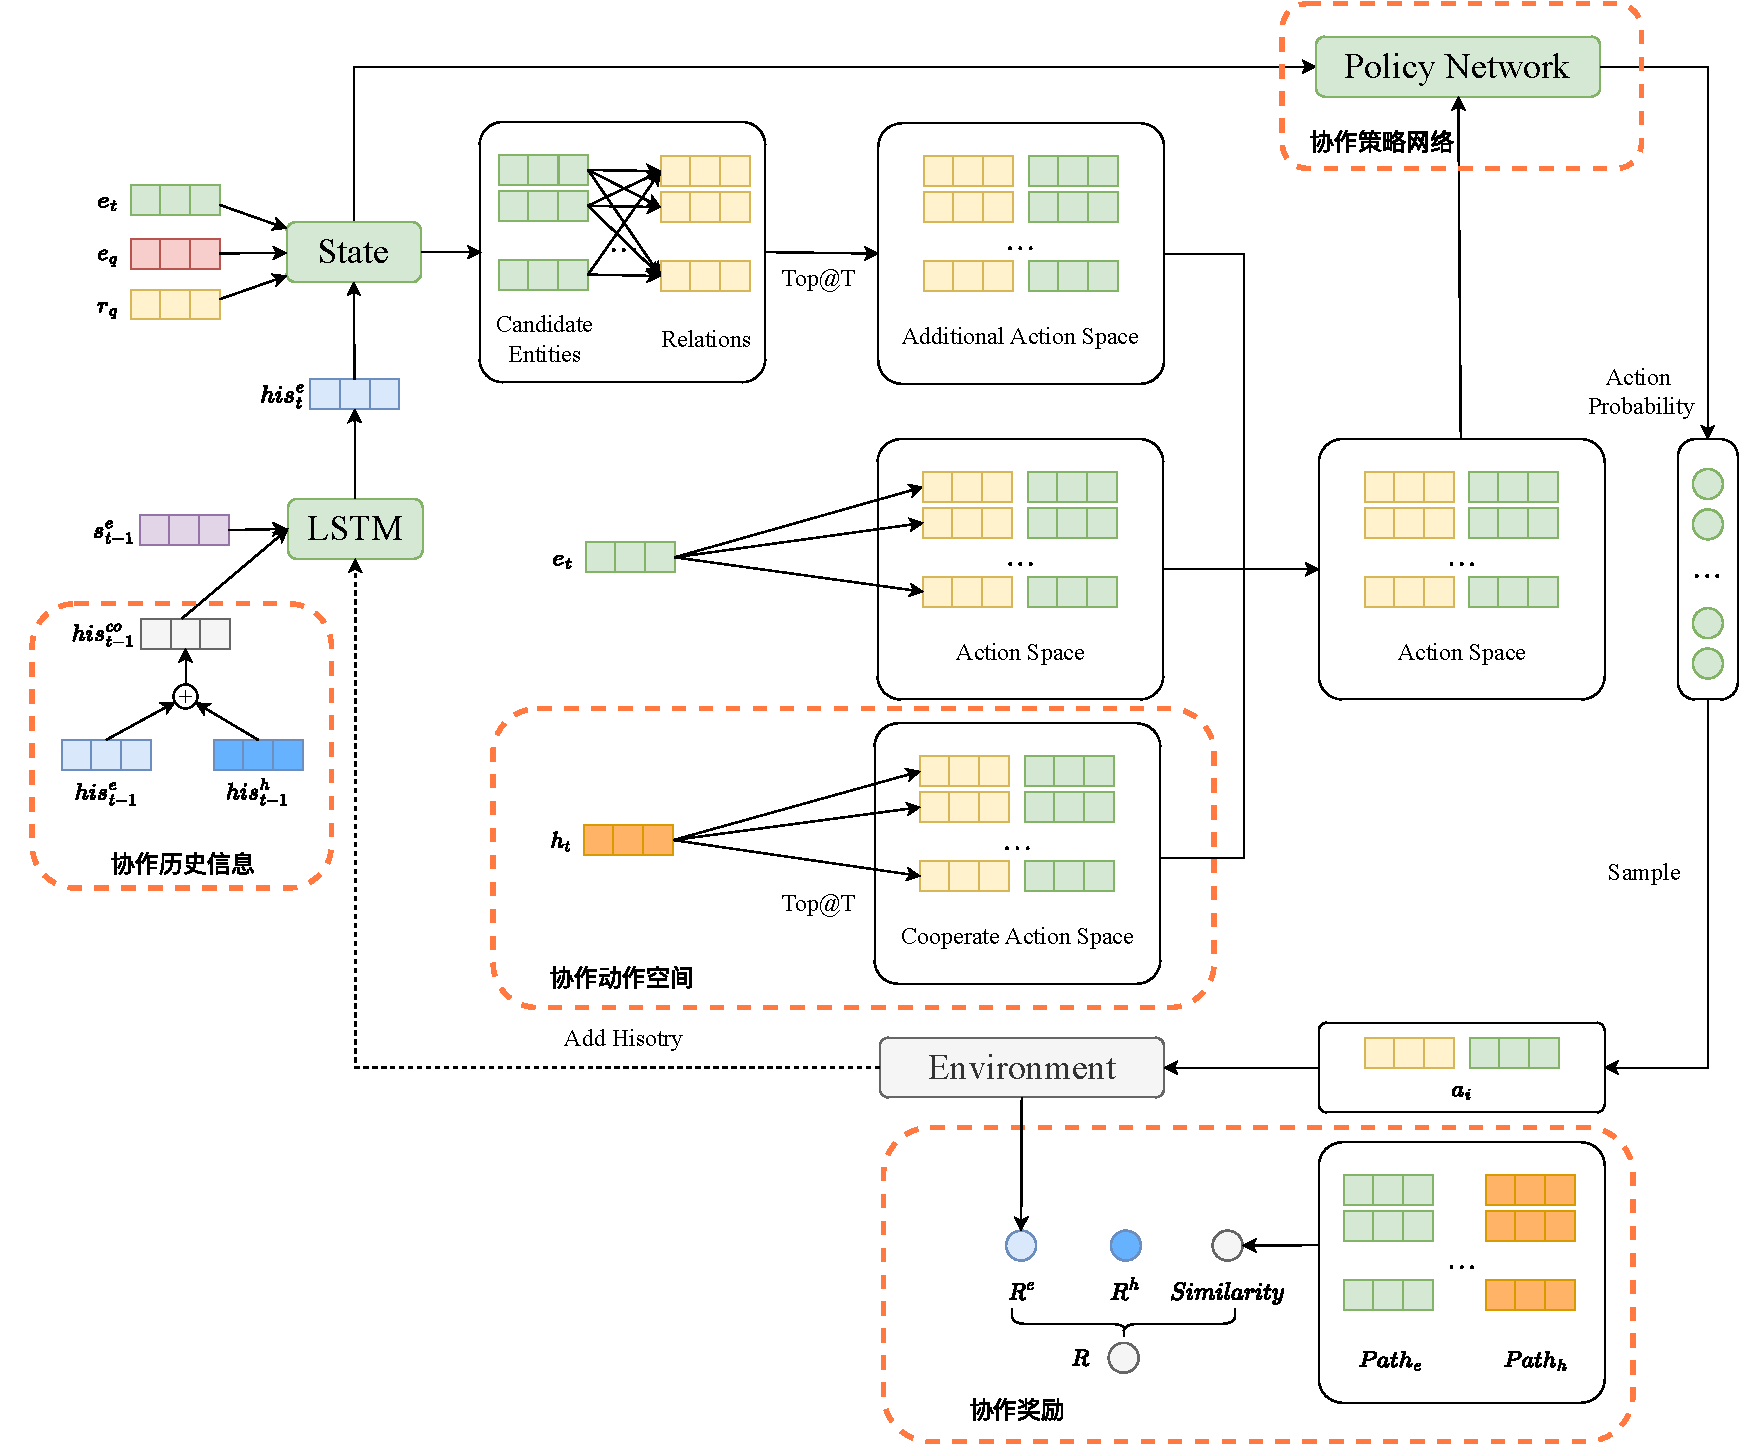
\includegraphics[width=0.8\textwidth]{3_LAURA_1}
    \label{3_LAURA_1}
  }

  \subfloat[大型智能体知识推理] {
    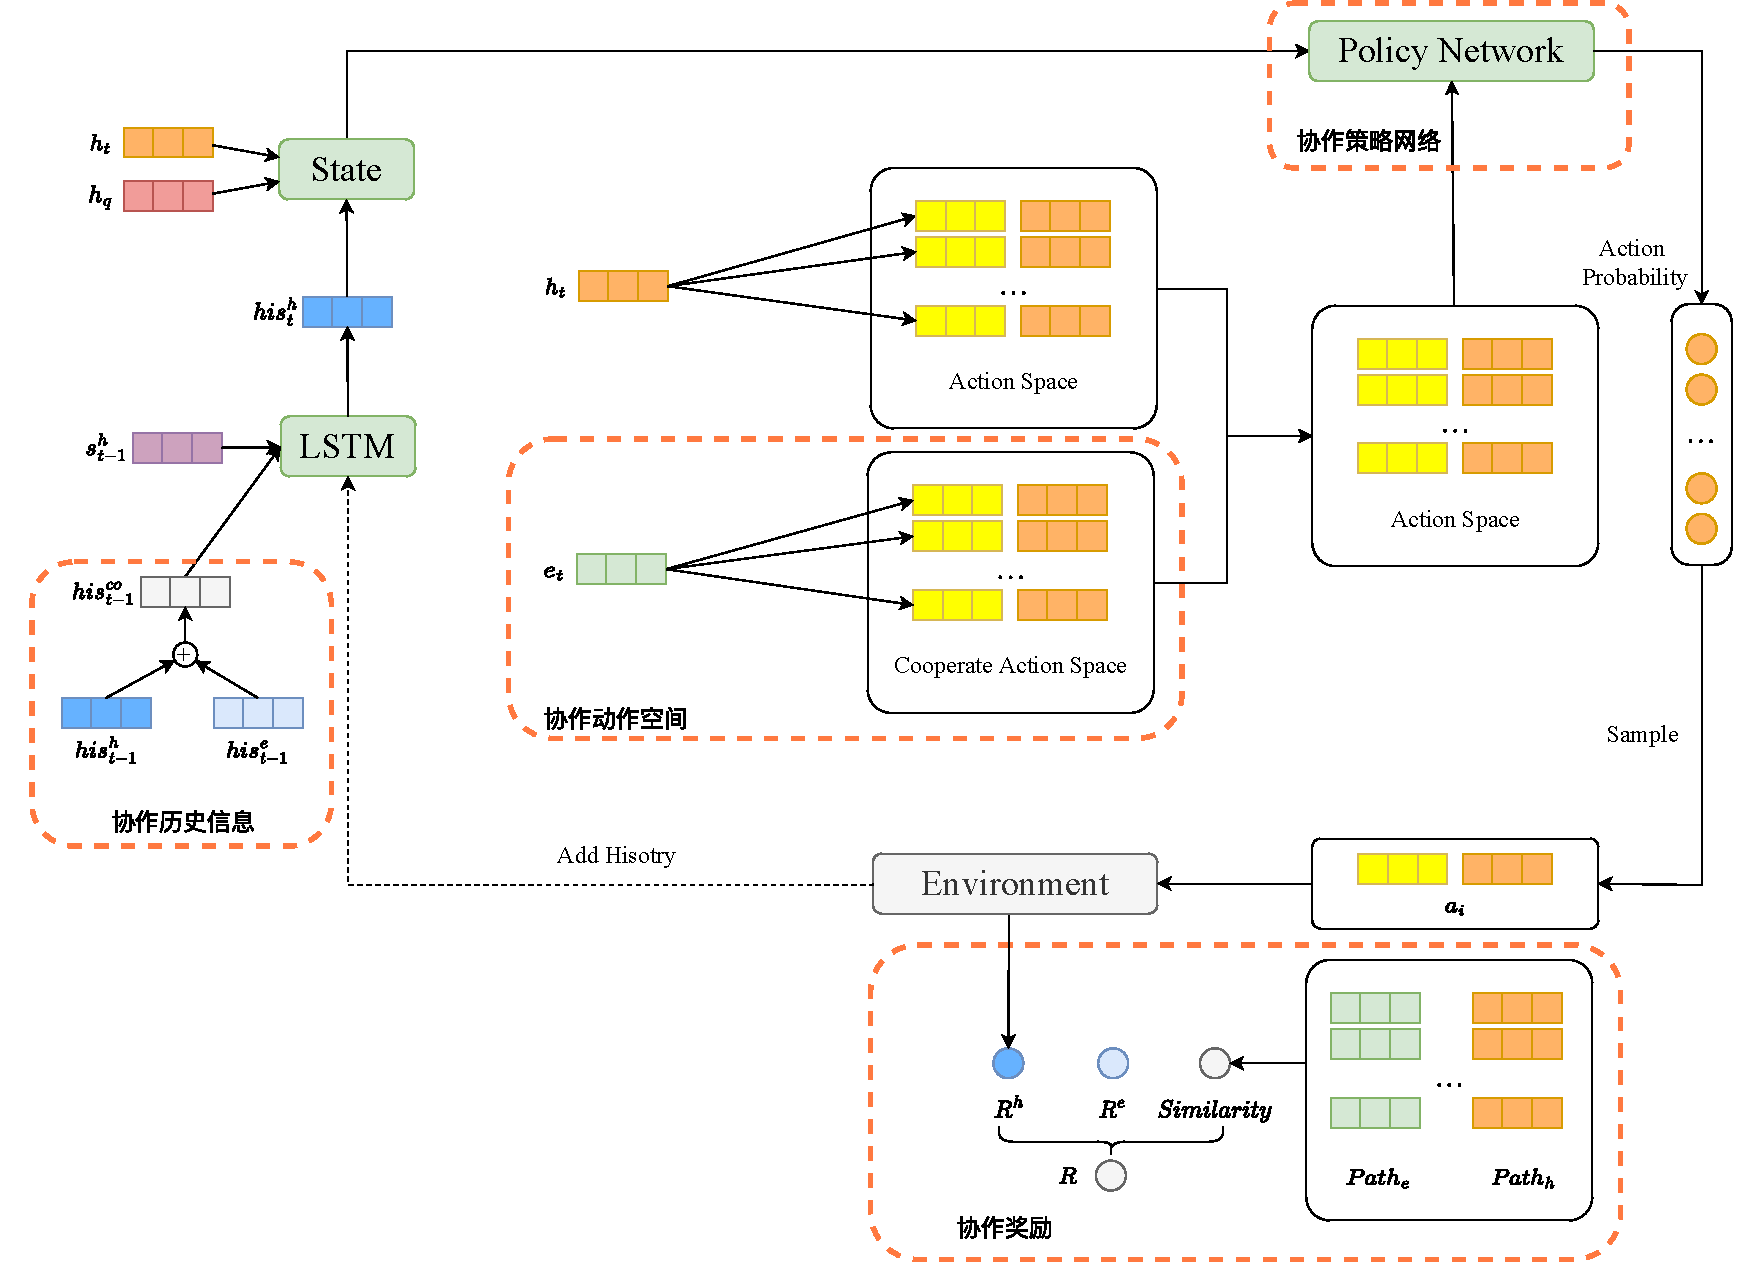
\includegraphics[width=0.8\textwidth]{3_LAURA_2}
    \label{3_LAURA_2}
  }
  \caption{基于双重智能体强化学习的知识推理模型框架图}
  \label{3_LAURA}
\end{figure}

\section{强化学习框架}
利用强化学习框架进行知识推理的过程可以认为是一种马尔可夫决策过程(Markov Decision Process,MDP)~\cite{gronauer2022multi}。
可以将知识推理过程表述为:给定知识图谱$G$的事实集合$F$和查询三元组$(h, r, ?)$(也可以是$(?, r, t)$和$(h, ?, t)$的形式),其中已知的实体可以记作查询实体$e_q$或第0跳实体$e_0$,给定关系可以记作查询关系$r_q$。
在强化学习框架中,智能体首先从查询实体$e_q$出发,由智能体不断选择知识图谱上的节点作为下一跳实体,直到到达跳数上限$L$为止,最终达到的实体即为知识推理结果,可以记为答案实体$e_a$。

具体而言,在强化学习框架的马尔可夫决策过程中,主要包含以下内容:
\begin{itemize}
  \item [1)] 状态信息$S$,主要用于表示智能体当前的状态情况。假设当前是智能体的推理过程的第$i$步,则智能体的状态信息可以表示为变量$\bm{s}_i = (\bm{e}_i, \bm{his}_i, \bm{e}_q, \bm{r}_q)$,其中$\bm{e}_i$表示第$i$步智能体所在实体的表示向量,$\bm{his}_i$表示智能体的历史轨迹信息表示向量,例如可以选择长短期记忆(Long Short-Term Memory,LSTM)模型编码智能体的历史轨迹并返回当前对应的表示向量$\bm{his}_i$,$\bm{e}_q$和$\bm{r}_q$则是查询实体和查询关系的表示向量,对单次查询而言是固定不变的信息。
  \item [2)] 动作空间$A$,是智能体当前所在实体节点$e_i$对应的知识图谱中全部出边构成的集合。当智能体处在实体节点$e_i$时,智能体的动作空间可以表示为变量$\bm{A}_i = \{(\hat{r}, \hat{e}) \mid (e_i, \hat{r}, \hat{e}) \in F\}$。
  \item [3)] 策略网络$\pi_\theta$,用于建模智能体的动作选择策略。策略网络$\pi_\theta$可以根据智能体当前的状态信息$\bm{s}_i$和动作空间$\bm{A}_i$给出各个动作的概率分布$\pi_\theta(a \mid \bm{s}_i, \bm{A}_i), a \in \bm{A}_i$,并通过随机采样的方式决定后续执行的动作。
  \item [4)] 状态转移过程,是智能体根据当前状态信息和动作空间,通过策略网络选择后续动作并更新状态信息的过程。当智能体根据策略网路选择了一个动作$a_i$后,有动作$a_i = (\hat{r}, \hat{e}), a_i \in \bm{A}_i$以及实体$e_{i+1}=\hat{e}$,同时智能体会更新自身的状态信息$\bm{s}_{i+1} = (\bm{e}_{i+1}, \bm{his}_{i+1}, \bm{e}_q, \bm{r}_q)$。
  \item [5)] 奖励函数$R$,用于根据智能体最终是否到达正确答案而提供相应的奖励。通常情况下的奖励函数$R$是一个二值函数,如果智能体达到了正确答案则提供奖励为1,否则提供奖励为0。
\end{itemize}

\subsection{小型智能体}
小型智能体能够在知识图谱上分析实体信息并进行知识推理。
在构建小型智能体的状态信息$\bm{s}_i$时,考虑到智能体需要能够获取三种信息,包括查询问题信息,当前节点信息和历史路径信息。其中,查询问题信息可以表示为查询三元组中的查询实体和查询关系对应的向量,即$\bm{e}_q$和$\bm{r}_q$。当前节点信息可以用当前实体对应的向量$\bm{e}_i$进行表示。对于历史路径信息,则考虑使用LSTM模型进行学习和表示。
令$L_e$表示小型智能体的最大推理步数,则历史信息对应的向量获取过程为:
\begin{equation}
  \bm{his}_i=\operatorname{LSTM}\left(\bm{his}_{i - 1}, \bm{s}_{i - 1}\right), i \in [1, L_e], i \in \mathbb{Z}
  \label{equation_HistoryLSTM}
\end{equation}
根据上述计算过程,最终得到的状态信息可以表示为$\bm{s}_i = (\bm{e}_i, \bm{his}_i, \bm{e}_q, \bm{r}_q)$。

随后进行动作空间的构造,具体构造过程如强化学习框架部分所述,主要是根据智能体所处的节点位置$e_i$和知识图谱事实集合$F$的三元组信息实现构建,可以表示为:
\begin{equation}
  \bm{A}_i = \{(\hat{r}, \hat{e}) \mid (e_i, \hat{r}, \hat{e}) \in F\}
  \label{base_1}
\end{equation}
在进行动作空间构建时,考虑到知识图谱可能存在节点链接稀疏的情况,造成智能体无法沿着链接路径进行高质量知识推理。
对此,本文根据历史路径信息和层次信息对动作空间进行扩展,并通过知识图谱表示学习模型NORMAN评估候选实体是否可行,构造额外动作空间$\bm{A}_{i}^{add}$。具体方法是将历史路径节点和当前实体的相同层次节点构建节点集合$E_i$,同时根据关系集合$R$构造候选动作。得到的额外动作空间$\bm{A}_{i}^{add}$可以表示为:
\begin{equation}
  \bm{A}_{i}^{add} = \{(\hat{r}, \hat{e}) \mid (e_i, \hat{r}, \hat{e}) \notin G, \hat{r} \in R, \hat{e} \in E_i \}
  \label{extra_1}
\end{equation}
随后将$\bm{A}_{i}^{add}$的动作与$e_i$构造成三元组集合,选择NORMAN模型对三元组进行打分和筛选,仅保留得分最高的$T$个三元组对应的动作,从而完成额外动作空间的筛选。这里设置$\operatorname{Top@T}$为保留得分最高的$T$个三元组的函数,则筛选后的额外动作空间$\bm{A}_{i}^{add}$可以表示为:
\begin{equation}
  \bm{A}_i^{add} = \{(\hat{r}, \hat{e}) \mid \operatorname{Top@T}(f_{\hat{r}}(e_i, \hat{e})), (e_i, \hat{r}, \hat{e}) \notin G, \hat{r} \in R, \hat{e} \in E_i \}
\end{equation}
最后进行空间的融合$\bm{A}_i = \bm{A}_i \cup \bm{A}_{i}^{add} $,完成动作空间的扩展操作。

在完成上述状态信息$\bm{s}_i$和动作空间$\bm{A}_i$的构造后,即可对小型智能体的状态转移过程进行分析。
在第$i$步推理过程时,小型智能体可以通过策略网络选择动作$\bm{a}_i = (\hat{r}, \hat{e}), \bm{a}_i \in \bm{A}_i$,并从实体$e_i$移动到$e_{i+1} = \hat{e}$。
小型智能体采用的策略网络可以表示为:
\begin{equation}
  \pi_\theta\left(\bm{a}_i \mid \bm{s}_i, \bm{A}_i\right) =\operatorname{Softmax}\left(\bm{A}_i \times \mathbf{W}_1 \operatorname{ReLU}\left(\mathbf{W}_2 \cdot \bm{s}_i\right)\right)
\end{equation}
其中$\mathbf{W}_1$和$\mathbf{W}_2$是待学习的参数。
随后,小型智能体会更新自身的状态信息$\bm{s}_{i+1} = (\bm{e}_{i+1}, \bm{his}_{i+1}, \bm{e}_q, \bm{r}_q)$,并进行下一步推理工作,直到达到最大步数$L_e$时停止知识推理。
此时即可得到答案实体$e_a$并返回知识推理路径$p_e$,完成知识推理过程。

在构建奖励函数$R$时,首先设置当智能体达到正确答案时奖励为1,不能达到正确答案时设置奖励为0。考虑到小型智能体在大规模知识图谱进行知识推理的过程中可能难以达到正确答案,会造成奖励稀疏的问题。因此当小型智能体没有到达正确答案时,本文利用第二章提出的NORMAN模型的得分函数$f_r(h, t)$计算知识推理结果$(e_q, r_q, e_a)$对应的得分,并将得分的数值范围缩放到$[0, 1)$区间内,作为智能体的奖励$R$。

\subsection{大型智能体}
大型智能体能够在聚类节点上进行知识推理,得到相应的推理路径并返回目标实体所在的聚类节点。
为了构建聚类知识图谱,本文首先使用NORMAN模型的层次信息提取部分对知识图谱进行表示学习,该模型为基于极坐标系的编码器,能够将实体和关系转换为极坐标系上的节点。随后采用K-Means聚类算法,根据实体的半径坐标向量将实体划分为$K$个层次级别,其中$K$为超参数,可以根据知识图谱进行调整。随后的聚类知识图谱构造过程为:对0到$K$的各个层次级别,分别将相同层次的实体构造为一个聚类实体。同时如果两个聚类实体的内部至少有一个关联知识存在,则为这两个聚类实体构造连接。通过上述步骤即可构建聚类知识图谱$G_h$。

完成聚类知识图谱构建后即可开始对大型智能体进行配置。这里设聚类知识图谱内的聚类实体为$h$,如第$i$跳实体可以表示为$h_i$。
首先在构建大型智能体的状态信息$\bm{s}_i$时,依然采用三种信息进行表示,分别是查询问题信息、当前节点信息和历史路径信息。
由于聚类知识图谱中的关系主要是描述不同聚类节点之间是否有内部联系,难以直接对查询三元组的查询关系$r_q$进行直接表示,因此在查询问题信息部分不加入查询关系信息,仅包含查询实体信息,表示为$\bm{h}_q$。
当前节点信息用当前聚类节点对应的向量$\bm{h}_i$表示。需要注意的是,这里是通过对聚类内全部实体向量取均值从而得到聚类节点的表示向量$\bm{h}_i$。
历史路径信息部分同样使用LSTM模型进行学习和表示,可以表示为:
\begin{equation}
  \bm{his}_i=\operatorname{LSTM}\left(\bm{his}_{i - 1}, \bm{s}_{i - 1}\right), i \in [1, L_h], i \in \mathbb{Z}
\end{equation}
最终构造的状态信息可以表示为$\bm{s}_i = (\bm{h_i}, \bm{his}_i, \bm{h}_q)$。

在进行动作空间的构造时,动作空间主要是根据大型智能体所处位置$h_i$和聚类知识图谱$G_h$的事实集合$F_h$进行构造,构造过程可以表示为:
\begin{equation}
  \bm{A}_i = \{(\hat{r}, \hat{h}) \mid (h_i, \hat{r}, \hat{h}) \in F_h\}
  \label{base_2}
\end{equation}
由于聚类知识图谱的节点较少,同时节点间的关系是根据节点内部实体是否存在关联知识而构建的,这就导致节点间的连接较多,智能体能够在稠密的知识图谱上进行遍历,从而使得大型智能体的动作空间较大。因此在构造大型智能体的动作空间时,不对动作空间进行额外扩充。

在完成上述状态信息$\bm{s}_i$和动作空间$\bm{A}_i$的构造后,即可对大型智能体在知识推理的过程中进行状态转移的过程进行分析。
在第$i$步推理的过程中,大型智能体通过策略网络选择动作$\bm{a}_i = (\hat{r}, \hat{h}), \bm{a}_i \in A_i$,并从聚类节点$h_i$转移到$h_{i+1}$。其中策略网络函数可以表示为:
\begin{equation}
  \pi_\theta\left(\bm{a}_i \mid \bm{s}_i, \bm{A}_i\right) =\operatorname{Softmax}\left(\bm{A}_i \times \mathbf{W}_1 \operatorname{ReLU}\left(\mathbf{W}_2 \cdot \bm{s}_i\right)\right)
\end{equation}
随后,更新大型智能体对应的状态信息$\bm{s}_{i+1} = (\bm{h}_{i+1}, \bm{his}_{i+1}, \bm{h}_q)$,并进行后续推理过程。
当大型智能体达到最大推理步数$L_h$时即可得到答案聚类节点$h_a$并返回推理路径$p_h$,完成推理过程。

最后进行奖励函数$R$的构造。由于聚类知识图谱的节点数量较少,这使得大型智能体达到正确实体所在的聚类节点的概率比小型智能体更高。因此大型智能体的奖励函数采用传统设计,即智能体最终到达正确聚类节点则奖励为1,没有到达则奖励为0。

\section{双重智能体知识推理}
本文提出的两种智能体均能够独立进行学习和训练,然而在知识推理效果上来看,小型智能体属于传统的强化学习知识推理方法,同时大型智能体只能在聚类知识图谱上进行知识推理,并最终确定答案实体所在的聚类节点,而不能确定真正的答案实体是哪一个。
因此,为了提高知识推理的效果,有必要将两种智能体结合起来,实现一种基于双重智能体强化学习的知识推理模型。
本文提出了协作动作空间、协作策略网络和协作奖励,能够将两种智能体结合起来,进而增强知识推理的效果。

\subsection{协作动作空间}
首先介绍协作动作空间,这种方法为每种智能体分别构造额外动作空间用于覆盖另一种智能体所在的节点,通过这种方法让两种智能体的动作空间相互交融,为两种智能体沿相似路径进行推理提供必要条件。
这里采用上角标$e$和$l$分别表示小型智能体和大型智能体对应的内容,$\bm{\hat{A}}_i$表示第$i$步的协作动作空间,则小型智能体在第$i$步的协作动作空间可以表示为:
\begin{equation}
  \bm{\hat{A}}_i^{e} = \{(\hat{r}, \hat{e}) \mid \hat{r} \in R, \hat{e} \in \operatorname{Entity}(h_i)\}
\end{equation}
其中,$\operatorname{Entity}(\cdot)$函数表示获取聚类节点对应的实体内容。
由于处于同一个聚类节点内的实体数量可能会很多,因此这里选择使用NORMAN模型对三元组进行打分和筛选,仅保留得分最高的$T$个三元组对应的动作,从而完成动作空间的筛选。
这里同样设置$\operatorname{Top@T}$为保留得分最高的$T$个三元组的函数,则筛选后的额外动作空间$\bm{A}_{i}^{add}$可以表示为:
\begin{equation}
  \bm{\hat{A}}_i^{e} = \{(\hat{r}, \hat{e}) \mid \operatorname{Top@T}(f_{\hat{r}}(e_i, \hat{e})), \hat{r} \in R, \hat{e} \in \operatorname{Entity}(h_i) \}
  \label{coo_1}
\end{equation}
通过上述函数,小型智能体的协作动作空间$\bm{\hat{A}}_i^{e}$可以包含大型智能体所在的聚类节点对应的实体节点,从而让小型智能体具有沿着大型智能体的路径继续前进的能力。
类似的,可以构造大型智能体在第$i$步的协作动作空间为:
\begin{equation}
  \bm{\hat{A}}_i^{h} = \{(\hat{r}, \hat{h}) \mid \hat{r} \in R_h, \hat{h} \in \operatorname{Hierarchy}(e_i)\}
  \label{coo_2}
\end{equation}
其中,$\operatorname{Hierarchy}(\cdot)$函数表示获取实体节点对应的层次级别。
通过上述函数,大型智能体的协作动作空间$\bm{\hat{A}}_i^{h}$也可以覆盖小型智能体所在的实体节点对应的聚类节点,从而大型智能体沿着与小型智能体相似的推理路径进行推理提供了支持。
最后,需要将协作动作空间合并到动作空间,完成动作空间的更新。这一过程可以表示为:
\begin{equation}
  \begin{aligned}
    \bm{A}_i^{e} &= \bm{A}_i^{e} \cup \bm{\hat{A}}_i^{e} \\
    \bm{A}_i^{h} &= \bm{A}_i^{h} \cup \bm{\hat{A}}_i^{h}
  \end{aligned}
\end{equation}

\subsection{协作策略网络}
协作策略网络的主要目标是结合两种智能体的状态信息和动作空间共同构建策略网络,使得一种智能体在选择动作时能够结合另一种智能体的信息,共同进行知识推理。
在具体的实践过程中,可以发现智能体的状态信息可以表示为$\bm{s}_i = (\bm{e}_i, \bm{his}_i, \bm{e}_q, \bm{r}_q)$。
其中$\bm{e}_i, \bm{e}_q, \bm{r}_q$分别是第$i$步智能体所在实体信息、查询实体信息和查询关系信息,这些信息基本只与智能体自身有关,难以与另一个智能体进行信息交互。
而历史信息$\bm{his}_i$可以通过调整与另一个智能体产生关联,从而进行信息交互。
因此,本文提出的协作策略网络首先构造协作历史信息$\bm{his}^{co}$,随后对两种智能体的历史信息进行计算,并进而构建协作策略网络。

这里设最大跳数为$L$,则可以通过两种智能体的历史信息拼接起来,构成智能体第$i$步的协作历史信息$\bm{his}_i^{co}$。协作历史信息的构建过程可以表示为:
\begin{equation}
  \bm{his}_{i}^{co} = \left[\bm{his}_{i-1}^e, \bm{his}_{i-1}^l\right], \quad i \in [1, L] \  \And \  i \in \mathbb{Z}
  \label{his_1}
\end{equation}

随后,采用LSTM模型对节点状态和协作历史信息一起进行编码,从而可以获得智能体的历史信息。小型智能体的历史信息向量的计算过程可以表示为:
\begin{equation}
  \begin{aligned}
    \bm{his}_0^e &= \operatorname{LSTM}^e\left(\bm{0}, \bm{0}\right) \\
    \bm{his}_i^e &= \operatorname{LSTM}^e\left(\mathbf{W}^e \cdot \bm{his}_i^{co}, \bm{s}_{i-1}^e\right),\quad i \in [1, L_e] \  \And \  i \in \mathbb{Z}
  \end{aligned}
  \label{his_2}
\end{equation}
可以采用相似的方法计算大型智能体的历史信息向量为:
\begin{equation}
  \begin{aligned}
    \bm{his}_0^l &=\operatorname{LSTM}^l\left(\bm{0}, \bm{0}\right) \\
    \bm{his}_i^l &= \operatorname{LSTM}^l\left(\mathbf{W}^l \cdot \bm{his}_i^{co}, \bm{s}_{i-1}^l\right),\quad i \in [1, L_h] \  \And \  i \in \mathbb{Z}
  \end{aligned}
  \label{his_3}
\end{equation}

完成历史信息的计算后,即可构建协作策略网络。
这里设置小型智能体的状态信息向量为$\bm{s}_i^{e} = \left[\bm{e}_q, \bm{r}_q, \bm{e}_i, \bm{his}_i^e\right]$,则构建的小型智能体的协作策略网络可以表示为:
\begin{equation}
  \pi_\theta^e\left(\bm{a}_i^e \mid \bm{s}_i^e, \bm{A}_i^e\right) =\operatorname{Softmax}\left(\bm{A}_i^e \times \mathbf{W}_1^e \operatorname{ReLU}\left(\mathbf{W}_2^e \cdot \bm{s}_i^{e}\right)\right)
  \label{pi_1}
\end{equation}
类似的,设置大型智能体状态信息向量为$\bm{s}_i^{h} = \left[\bm{h}_q, \bm{h}_i, \bm{his}_i^l\right]$,可以构建大型智能体的协作策略网络。
\begin{equation}
  \pi_\theta^l\left(\bm{a}_i^l \mid \bm{s}_i^l, \bm{A}_i^l\right) =\operatorname{Softmax}\left(\bm{A}_i^l \times \mathbf{W}_1^l \operatorname{ReLU}\left(\mathbf{W}_2^l \cdot \bm{s}_i^{h}\right)\right)
  \label{pi_2}
\end{equation}

通过上述方法构建的协作策略网络,可以为智能体提供动作空间内各项动作的概率,并通过采样的方式获取后续动作,实现知识推理。
在这些步骤中,通过构建协作历史信息$\bm{his}^{co}$,可以让两种智能体共享历史路径信息,从而有助于帮助它们协作推理,共同解决问题。
具体而言,大型智能体会提供给小型智能体当前层次的信息,并帮助小型智能体确定接下来的动作应该朝着高层次还是低层次的方向进行推理。
另一方面,小型智能体会为大型智能体分享当前的实体信息,帮助大型智能体了解后续动作应该朝带有何种实体特征的聚类节点前进。
通过上述方法,两种智能体能够相互协作,并获取正确的知识推理路径。

\subsection{协作奖励}
上面提出的协作动作空间能够为两种智能体沿着相似的轨迹行进提供了必要条件,协作策略网络能够帮助两种智能体交换信息。
但是上述方法均不能明确地指导两种智能体需要沿着相似的路径进行推理,这导致两种智能体依然只会考虑自身能否到达目标节点,而没有考虑帮助另一个智能体达到正确的节点。

为了进一步增强两种智能体的协作,本节设计的协作奖励能够作为一种补充奖励,鼓励两种智能体沿着相似的路径推理。协作奖励的思路主要是:对两种智能体推理的路线进行相似度计算,并获取相似度得分。此外,还需要加上另一种智能体的原始得分,以评估是否智能体提供的指导信息能够帮助另一个智能体得到正确的答案。

在计算的过程中,采用$\hat{R}_i$表示第$i$步的协作奖励得分,则小型智能体的协作奖励可以表示为:
\begin{equation}
  \hat{R}^e = \sum_{i=1}^{L} \operatorname{Similarity}(\bm{e}_i, \bm{h}_i) + R^h
  \label{similar_1}
\end{equation}
其中$\operatorname{Similarity}(\cdot)$是相似度评估函数,主要计算方法是对输入的两个向量的余弦相似度进行计算。
需要注意的是,这里聚类节点的向量是通过对聚类内全部实体的向量求均值得到的。
类似的,可以构建大型智能体的协作奖励:
\begin{equation}
  \hat{R}^h = \sum_{i=1}^{L} \operatorname{Similarity}(\bm{e}_i, \bm{h}_i) + R^e
  \label{similar_2}
\end{equation}

最后,对两种智能体的奖励函数进行更新,即可完成奖励函数的补充:
\begin{equation}
  \begin{aligned}
    R^e &= R^e + \hat{R}^e \\
    R^h &= R^h + \hat{R}^h
  \end{aligned}
  \label{similar_reward}
\end{equation}

协作奖励能够通过计算推理路径的余弦相似度,评估两种智能体是否沿相似路径进行推理。同时协作奖励还考虑了另一种智能体的最终得分,因此能够在保证推理路径相近的情况下,兼顾对另一个智能体正确性的观察。此外,协作奖励还有助于缓解大规模知识图谱中应用强化学习框架的奖励稀疏问题,提高智能体的学习速度。

\begin{algorithm}[H]
	\caption{LAURA模型训练算法}  
	\label{algorithm_dualagent}
	\begin{algorithmic}[1]
  \Require 知识图谱事实集合$F$, 聚类知识图谱事实集合$F_h$, 数据集$D$, NORMAN模型$M$, 最大范围$L$, 学习率$\alpha$
  \Ensure 小型智能体策略网络$\pi_\theta^e$, 大型智能体策略网络$\pi_\theta^l$
  \For{$(e_q, r_q, e_a) \in D$} 
  \State $(h_q, h_a) \leftarrow \operatorname{GetCluterNode}(e_q, e_a)$ // 获取大型智能体的查询节点和查询答案
  \State $\bm{s}_{0}^{e} \leftarrow (\bm{e}_q, \bm{0}, \bm{e}_q, \bm{r}_q), \bm{s}_{0}^{l} \leftarrow (\bm{h}_q, \bm{0}, \bm{h}_q)$ // 初始化状态信息
  \State $\bm{A}_{0}^{l} \leftarrow \operatorname{GetActionSpace}(h_0, F_h) \cup \operatorname{GetCooperationSpace}(h_0, e_0)$ \par\quad// 根据公式\ref{base_2}和\ref{coo_2}获取大型智能体动作空间
  \State $\bm{A}_{0}^{e} \leftarrow \operatorname{GetActionSpace}(e_0, F) \cup \operatorname{GetExtraSpace}(e_0, M) \cup \operatorname{GetCooperationSpace}(e_0, h_0)$ \par\quad// 根据公式\ref{base_1}, \ref{extra_1}和\ref{coo_1}获取小型智能体动作空间
  \For{$i \leftarrow 1$ to $L$}
  \State $\bm{h}_i \leftarrow \operatorname{Sample}(\pi_\theta^l(\bm{s}_{i-1}^{l}, \bm{A}_{i-1}^{l}))$ // 策略网络采样获取新的聚类节点
  \State $\bm{e}_i \leftarrow \operatorname{Sample}(\pi_\theta^e(\bm{s}_{i-1}^{e}, \bm{A}_{i-1}^{e}))$ // 策略网络采样获取新的实体节点
  \State $\bm{his}_{i}^{coo} \leftarrow \operatorname{GetHistory}(\bm{his}_{i-1}^{e}, \bm{his}_{i-1}^{l})$ // 根据公式\ref{his_1}获取协作历史信息
  \State $\bm{his}_{i}^{l} \leftarrow \operatorname{GetHierarchyHistory}(\bm{his}_{i}^{coo}, \bm{h}_{i-1})$ \par\quad\quad // 根据公式\ref{his_3}获取大型智能体历史信息
  \State $\bm{his}_{i}^{e} \leftarrow \operatorname{GetEntityHistory}(\bm{his}_{i}^{coo}, \bm{e}_{i-1})$ \par\quad\quad // 根据公式\ref{his_2}获取小型智能体历史信息
  \State $\bm{s}_{i}^{l} \leftarrow (\bm{h}_{i}, \bm{his}_{i}^{l}, \bm{h}_q)$ // 更新大型智能体状态信息
  \State $\bm{s}_{i}^{e} \leftarrow (\bm{e}_{i}, \bm{his}_{i}^{e}, \bm{e}_q, \bm{r}_q)$ // 更新小型智能体状态信息
  \State $\bm{A}_{i}^{l} \leftarrow \operatorname{GetActionSpace}(\bm{h}_i, F) \cup \operatorname{GetCooperationSpace}(\bm{h}_i, \bm{e}_i)$ \par\quad\quad// 更新大型智能体动作空间
  \State $\bm{A}_{i}^{e} \leftarrow \operatorname{GetActionSpace}(\bm{e}_i, F) \cup \operatorname{GetExtraSpace}(\bm{e}_i, M) \cup \operatorname{GetCooperationSpace}($\par\quad\quad$\bm{e}_i, \bm{h}_i)$ // 更新小型智能体动作空间
  \EndFor
  \State $R^{l} \leftarrow \operatorname{GetLayerReward}(\bm{h}_L, \bm{h}_a) + \operatorname{GetSimilarReward}_{i=1,\cdots,L_l}(\bm{e}_i, \bm{h}_i) + R^{e}$ \par\quad // 根据公式\ref{similar_2}和\ref{similar_reward}计算大型智能体奖励
  \State $R^{e} \leftarrow \operatorname{GetEntityReward}(\bm{e}_L, \bm{e}_a, M) + \operatorname{GetSimilarReward}_{i=1,\cdots,L_e}(\bm{e}_i, \bm{h}_i) + R^{l}$ \par\quad // 根据公式\ref{similar_1}和\ref{similar_reward}计算小型智能体奖励
  \State $\pi_\theta^l \leftarrow \operatorname{UpdatePolicyNetwork}(\pi_\theta^l, R^{l}, \alpha)$// 更新大型智能体策略网络
  \State $\pi_\theta^e \leftarrow \operatorname{UpdatePolicyNetwork}(\pi_\theta^e, R^{e}, \alpha)$// 更新小型智能体策略网络
  \EndFor
  \State \Return $\pi_\theta^e, \pi_\theta^l$
	\end{algorithmic}
\end{algorithm} 

\subsection{知识推理过程}
在完成了两种智能体的构建,并采用了协作动作空间、协作策略网络和协作奖励后,即可进行LAURA模型的训练。
基于双重智能体强化学习的知识推理模型LAURA的训练过程如算法\ref{algorithm_dualagent}所示。
可以发现,在知识推理过程中首先从数据集中取出对应的查询实体、查询关系和查询答案,这些信息可以直接提供给小型智能体。同时根据聚类的结果获取查询实体和查询答案所在的聚类节点,从而得到大型智能体的查询实体和查询答案。
随后根据上述信息初始化两种智能体的状态信息,并构建动作空间。随后即可进行知识推理过程,这里设置两种智能体的推理步数上限为$L$,则后面需要进行$L$步的知识推理。在每一步知识推理中,首先由大型智能体进行单步知识推理,随后由小型智能体进行单步知识推理,单步知识推理就是由策略网络进行采样获取相应的动作,并获取动作中的实体作为当前的节点。随后进行协作历史信息的获取,并更新两种智能体的历史信息,进而更新智能体的状态信息,以及构建新的动作空间。当完成了$L$步的知识推理后,需要对两种智能体进行奖励的计算,包含了智能体本身的奖励和协作奖励,其中协作奖励又包括两种智能体知识推理路径的相似度和另一个智能体的奖励。最后通过奖励对智能体的策略网络进行更新。完成模型训练后,即可得到最终的策略网络,此时智能体可以根据输入的查询信息进行推理,并得到合适的知识推理路径。

可以发现,LAURA模型训练过程中与知识图谱表示学习NORMAN结合紧密,能够通过NORMAN模型扩展智能体的动作空间以及补充智能体的奖励。
同时可以发现,本节提出的协作动作空间、协作策略网络和协作奖励能够将两种智能体结合起来,确保两种智能体能够接受对方信息并沿着与对方相似的推理路径进行知识推理,实现了实体和层次信息的相互交流和知识推理轨迹的相互协调,从而保障了知识推理的质量。

\section{实验评估}
本节在多个开源数据集上开展实验,综合评估LAURA模型的性能。
LAURA模型使用Python语言编写,Python版本为3.10.1,使用的深度学习框架为PyTorch,版本为1.13.1。
同时,本节所有实验都是在型号为AMAX G448-X3的服务器上完成的,服务器的具体参数包括:CPU型号为Xeon Sliver 4314,GPU型号为GeForce RTX 3090,系统内存为64G,系统硬盘为500G,操作系统版本为Ubuntu 22.04.1 LTS。

\subsection{实验概览}
知识推理模型的目标是基于知识图谱中的已有知识预测和推理新的知识。为了评估知识推理模型的效果,本文重点选择了单跳知识图谱问答和多跳知识图谱问答任务来进行模型评估。
在单跳知识图谱问答任务中,知识推理模型可以直接采用查询语句进行单跳知识推理,对于不能直接知识推理的模型则首先需要通过知识抽取将查询语句转换成查询三元组$(h, r, ?)$,$(?, r, t)$或$(h, ?, t)$,随后的知识推理过程和知识图谱补全的过程较为相似,通过知识推理模型对所有候选答案进行评分,这里的获取得分有多种方法,可以是知识图谱表示学习模型的得分函数,也可以是强化学习等推理模型通过计算得到的置信度得分。最后按照得分的降序顺序对候选三元组进行排序,并根据结果三元组序列评估模型效果。
多跳知识图谱问答则相对更加复杂一些。知识推理模型可以直接采用查询语句进行多跳知识推理,对于不能直接知识推理的模型也是需要将查询语句转换成查询三元组$(h, r, ?)$,$(?, r, t)$或$(h, ?, t)$,随后要求模型根据已有的知识图谱进行查询,在指定跳数的范围内进行多跳推理,最后对所有候选答案进行得分计算,同样是对得分进行降序排序,并根据最终排序结果评估模型效果。同时,多跳知识图谱问答要求模型能够提供相应的推理路径,从而能够对模型推理过程的充分性和合理性进行评估。

在构造查询语句时,本文首先采用了与知识图谱补全任务相似的方式,通过随机移除知识图谱事实三元组$(h, r, t)$中的任意一项构造查询三元组。
随后需要利用查询三元组构造对应的查询语句,考虑到实验的主要目的是考察模型的知识推理效果而不是知识抽取效果,因此本文采用固定的模板构造统一格式的查询语句。对于$(h, r, ?)$格式的查询三元组,构造的查询语句为“\textit{$h$的$r$是什么?}”。对于$(?, r, t)$格式的查询三元组,构造的查询语句为“\textit{$t$的$r^{-1}$是什么?}”,其中$r^{-1}$表示关系$r$的逆关系。对于$(h, ?, t)$格式的查询三元组,构造的查询语句为“\textit{$h$和$t$的关系是什么?}”。通过上述模板,可以将查询三元组转换为查询语句。同时,模型采用的知识抽取过程也是采用模板匹配的方法,通过对上述查询语句应用模板进行匹配获取对应的查询三元组,并完成后续的知识推理工作。
本文选择的知识图谱问答的评价指标同样为平均排序MR、平均倒数排序MRR和Hits@K等,根据知识图谱补全实验的分析,一般认为平均倒数排序MRR的表示能力优于平均排序MR,因此本文选择平均倒数排序MRR和Hits@K作为评估指标。

本节首先介绍了知识推理模型的评估实验内容,即通过单跳知识图谱问答和多跳知识图谱问答评估模型的效果。随后介绍了任务的评价指标、数据集和具体的实验设置,并在比较了本文提出的LAURA模型和其他基线知识推理模型在知识图谱问答上的效果,进而对LAURA模型的优势和劣势进行客观评估。

\subsection{数据集}
\begin{table}[t]
  \centering
  \caption{单跳知识图谱问答数据集统计信息}
  \begin{tabular*}{0.95\textwidth}{@{\extracolsep{\fill}}lccccc}
    \toprule[1pt]
    数据集 & 实体数量 & 关系数量 & 训练集数量 & 验证集数量 & 测试集数量 \\ \hline
    FB15K-237 & 14541 & 237 & 272115 & 17535 & 20466\\
    WN18RR & 40943 & 11 & 86835 & 3034 & 3134\\
    NELL-995 & 75492 & 200 & 138793 & 7710 & 7710\\
    \bottomrule[1pt]
	\end{tabular*}
  \label{Datasets1_1}
\end{table}

\subsection{数据集}
\begin{table}[t]
  \centering
  \caption{多跳知识图谱问答数据集统计信息}
  \begin{tabular*}{0.95\textwidth}{@{\extracolsep{\fill}}lccccc}
		\toprule[1pt]
    数据集 & 实体数量 & 关系数量 & 训练集数量 & 验证集数量 & 测试集数量 \\ \hline
    FB15K-237-10\% & 11512 & 237 & 27211 & 15624 & 18150\\
    FB15K-237-20\% & 13166 & 237 & 54423 & 16963 & 19776\\
    FB15K-237-50\% & 14149 & 237 & 136057 & 17449 & 20324\\
		\bottomrule[1pt]
	\end{tabular*}
  \label{Datasets2}
\end{table}
本文在单跳知识图谱问答和多跳知识图谱问答两种任务上进行模型评估。
针对单跳知识图谱问答,本文采用的数据集包括:FB15K-237、WN18RR和NELL-995。
另一方面,对于多跳知识图谱问答,本文采用的数据集包括:FB15K-237-10\%、FB15K-237-20\%和FB15K-237-50\%~\cite{lv2020dynamic}。
在单跳知识图谱问答中,由于单跳知识图谱问答与知识图谱补全任务对数据集的要求是相同的,因此本文选择与知识图谱表示学习模型实验部分相同的数据集,即FB15K-237、WN18RR和NELL-995,从而能够更好的对本文提出的两种模型进行对比。
在多跳知识图谱问答任务中,考虑到多跳推理过程需要综合一定范围内的知识进行综合评估,为了测试本文提出的模型在不同稀疏程度的知识图谱上的性能,本文选择了多个基于FB15K-237数据集进行随机采样得到的数据集,即FB15K-237-10\%、FB15K-237-20\%和FB15K-237-50\%。由名字可以看出,这三个数据集分别随机保留了FB15K-237数据集的10\%、20\%和50\%的三元组数据,从而能够评估模型利用不同稀疏程度的知识图谱进行知识推理的能力。同时,在稀疏的知识图谱上进行多跳知识图谱问答是一种复杂的知识推理任务,能够充分的评估各种模型的性能。
具体统计数量上,本部分采用的单跳推理测试数据集的统计数据如表\ref{Datasets1_1}所示,多跳推理测试数据集如表\ref{Datasets2}所示。根据上文分析可知,本文选择的单跳和多跳知识图谱问答数据集能够较好的评估模型的知识推理能力,同时能够评估模型在不同稀疏程度的知识图谱上的效果。

\begin{table}[t]
  \centering
  \caption{单跳知识图谱问答超参数设置情况}
  \begin{tabular*}{0.95\textwidth}{@{\extracolsep{\fill}}lcccc}
    \toprule[1pt]
    \multirow{2}{*}{超参数名称} & \multirow{2}{*}{取值范围} & \multicolumn{3}{c}{最佳超参数}\\ 
      &  & FB15K-237 & WN18RR & NELL-995 \\ \hline
    动作丢弃率 & $\{0, 0.1, 0.2, 0.5, 0.8\}$ & 0.5 & 0.2 & 0.2 \\
    集束搜索大小 & $\{32, 64, 128, 256, 512\}$ & 256 & 128 & 128 \\
    $\alpha$ & $\{1e\text{-}3, 2e\text{-}4, 5e\text{-}5, 2e\text{-}5\}$ & $1e\text{-}3$ & $1e\text{-}3$ & $1e\text{-}3$ \\
    $T$ & $\{0, 2, 4, 6, 8\}$ & 2 & 4 & 4 \\
    $K$ & $\{25, 50, 75, 100, 125\}$ & 50 & 75 & 75\\
    \bottomrule[1pt]
  \end{tabular*}
  \label{Hyperparameters2_Singlehop}
\end{table}

\begin{table}[t]
  \centering
  \caption{多跳知识图谱问答超参数设置情况}
  \begin{tabular*}{0.95\textwidth}{@{\extracolsep{\fill}}lcccccc}
    \toprule[1pt]
    \multirow{2}{*}{超参数名称} & \multirow{2}{*}{取值范围} & \multicolumn{3}{c}{最佳超参数}\\ 
      &  & \small{FB15K-237-10\%} & \small{FB15K-237-20\%} & \small{FB15K-237-50\%} \\ \hline
    动作丢弃率 & $\{0, 0.1, 0.2, 0.5, 0.8\}$ & 0.5 & 0.5 & 0.5 \\
    集束搜索大小 & $\{32, 64, 128, 256, 512\}$ & 512 & 256 & 256 \\
    $\alpha$ & $\{1e\text{-}3, 2e\text{-}4, 5e\text{-}5, 2e\text{-}5\}$ & $1e\text{-}3$ & $1e\text{-}3$ & $1e\text{-}3$ \\
    $T$ & $\{0, 2, 4, 6, 8\}$ & 8 & 6 & 4 \\
    $K$ & $\{25, 50, 75, 100, 125\}$ & 50 & 50 & 50\\
    \bottomrule[1pt]
  \end{tabular*}
  \label{Hyperparameters2_Multihop}
\end{table}

\subsection{基线模型}
本文选择了一些表现较好的方法作为基线模型进行对比:
\begin{itemize}
  \item [1)]\textbf{TransE:}Bordes等~\cite{bordes2013translating}提出的TransE模型是最经典的翻译模型,通过基于距离的评分函数将关系作为头实体和尾实体间的翻译,并将翻译后的两个实体间的距离作为得分,从而获取三元组的合理性。
  \item [2)]\textbf{ComplEx:}Trouillon等~\cite{trouillon2016complex}提出的ComplEx模型是对DistMult的一种扩展,通过使用复数嵌入能够建模不对称关系并实现效果提升。
  \item [3)]\textbf{ConvE:}Dettmers等~\cite{dettmers2018convolutional}提出的ConvE模型是一种卷积神经网络神经推理模型,能够通过二维卷积捕获实体间的特征交互信息并实现知识推理。
  \item [4)]\textbf{pLogicNet:}Qu等~\cite{qu2019probabilistic}提出的pLogicNet模型是一种符号推理模型,综合了马尔可夫符号网络MLN和图嵌入技术的思想,能够处理知识图谱中的缺失信息和实现高效知识推理。
  \item [5)]\textbf{NeuralLP:}Yang等~\cite{yang2017differentiable}提出的NeuralLP模型是一种基于矩阵的神经符号推理模型,能够在知识推理过程中得到带有权重的链式逻辑规则,并通过注意力机制实现规则信息的聚合和实现推理路径的评分。
  \item [6)]\textbf{MINERVA:}Das等~\cite{das2018go}提出的MINERVA模型是采用强化学习框架的神经符号推理模型,智能体可以从查询实体出发遍历各个路径实现知识推理。
  \item [7)]\textbf{M-Walk:}Shen等~\cite{shen2018m}提出的M-Walk模型同样采用强化学习框架,同时采用了一种基于价值的强化学习方法,并使用蒙特卡洛树搜索来改善奖励稀疏的问题。
\end{itemize}
其中,TransE和ComplEx均为知识图谱表示学习模型,可以通过模型的评分函数对单跳知识图谱问答的目标三元组进行打分,实现单跳知识图谱问答。
ConvE、pLogicNet、NeuralLP、MINERVA和M-Walk则为知识推理模型,除了能够进行单跳知识图谱问答任务外还可以执行多跳知识图谱问答任务,并提供知识推理路径信息。

\subsection{实验设置}
在使用LAURA模型进行单跳和多跳知识图谱问答实验前,首先需要对模型的超参数进行设置。本文对LAURA模型的超参数进行了调整,并最终形成了一系列最优超参数。
首先,需要针对强化学习框架设置超参数。这里设置最大出边度数为200,最大动作空间为256,实体对最大边数为10,实体嵌入维度为512,嵌入丢弃率为0.3,前馈层丢弃率为0.1,历史网络层数为3,历史嵌入维度为128,衰减率为0.05,延迟复制步数为5,采样部署频率为3,训练批次大小为128。
考虑到各个数据集的数据量大小和结构差异,针对不同的数据集还需要设置对应的动作丢弃率、集束搜索(beam search)大小和学习率$\alpha$。
随后需要设置小型智能体的最大跳数$L_e$和补充动作空间大小$T$。这里统一设置$L_e = 3$。
类似的,需要对大型智能体知识图谱问答的最大跳数$L_h$进行设置。同样也是设置为$L_h = 3$。
同时,需要为大型智能体构造聚类知识图谱,因此需要设置K-Means聚类的数量$K$。
由于LAURA需要使用NORMAN模型提供知识图谱层次信息,以及使用NORMAN模型的得分函数作为补充奖励,因此还需要对NORMAN模型的超参数进行设置。考虑到单跳知识图谱问答同样使用了FB15K-237、WN18RR和NELL-995数据集,因此采用的超参数设置情况与表\ref{Hyperparameters1}相同。多跳知识图谱问答部分则需要重新设置对应的NORMAN模型超参数。在对FB15K-237-10\%、FB15K-237-20\%和FB15K-237-50\%进行超参数调整和实验评估后,最后的超参数仍然与FB15K-237一致。
实验针对单跳知识图谱问答和多跳知识图谱问答分别调整对应超参数,得到的超参数设置情况分别如表\ref{Hyperparameters2_Singlehop}和表\ref{Hyperparameters2_Multihop}所示。

\subsection{实验结果与分析}
\subsubsection{单跳知识图谱问答实验}

\begin{table}[t]
  \centering
  \caption{FB15K-237数据集单跳知识图谱问答实验结果}
  \begin{tabular*}{0.95\textwidth}{@{\extracolsep{\fill}}lcccc}
    \toprule[1pt]
    \multirow{2}{*}{模型} & \multicolumn{4}{c}{FB15K-237}   \\
      & MRR & Hits@1 & Hits@3 & Hits@10 \\ \hline
    TransE & 29.4 & 24.8 & 40.1 & 46.5 \\
    ComplEx & 24.7 & 15.8 & 27.5 & 42.8 \\
    ConvE & 32.5 & 23.7 & 34.7 & 50.1 \\
    pLogicNet & 33.2 & 23.7 & 36.2 & 52.8 \\
    NeuralLP & 22.7 & 16.6 & 24.8 & 34.8 \\
    MINERVA & 27.1 & 19.2 & 30.7 & 42.6 \\
    M-Walk & 23.4 & 16.8 & 24.5 & 40.3 \\
    LAURA & \textbf{38.2} & \textbf{26.1} & \textbf{43.9} & \textbf{57.6} \\
    \bottomrule[1pt]
  \end{tabular*}
  \label{Experiment2_FB15K-237}
\end{table}
在FB15K-237数据集中采用上述模型执行单跳知识图谱问答,得到的实验结果如表\ref{Experiment2_FB15K-237}所示。可以发现本文提出的LAURA模型能够取得最好的成绩。
需要注意的是,在FB15K-237数据集中知识推理模型容易陷入中心节点而无法获取到正确的答案。与其他知识推理模型不同的是,LAURA模型与知识图谱表示学习模型NORMAN进行了融合,能够使用NORMAN模型完成额外动作空间的构建,并使用NORMAN模型的评分函数提供没有到达正确答案时的奖励。因此,通过上述方法可以让LAURA模型获取到NORMAN模型提供的额外信息,从而提高LAURA模型的效果。
同时,LAURA模型还采用了双重智能体强化学习的方式,能够利用大型智能体知识推理获取层次信息,并通过协作动作空间、协作策略网络和协作奖励将层次信息提供给小型智能体。通过上述方式能够帮助小型智能体在面对具有大量出边的中间节点时寻找正确的推理方向,最终达到答案实体,从而提高LAURA模型在FB15K-237知识图谱上的效果。

\begin{table}[t]
  \centering
  \caption{WN18RR数据集单跳知识图谱问答实验结果}
  \begin{tabular*}{0.95\textwidth}{@{\extracolsep{\fill}}lcccc}
    \toprule[1pt]
    \multirow{2}{*}{模型} & \multicolumn{4}{c}{WN18RR}   \\
      & MRR & Hits@1 & Hits@3 & Hits@10 \\ \hline
    TransE & 22.6 & 28.9 & 46.4 & 50.4 \\
    ComplEx & 44.5 & 41.2 & 46.3 & 51.0 \\
    ConvE & 43.2 & 40.5 & 44.1 & 52.4 \\
    pLogicNet & 44.1 & 39.8 & 43.4 & 53.7 \\
    NeuralLP & 45.9 & 37.6 & 46.8 & \textbf{65.7} \\
    MINERVA & 44.8 & 41.3 & 45.6 & 51.3 \\
    M-Walk & 43.7 & 41.5 & 44.7 & 54.3 \\
    LAURA & \textbf{47.1} & \textbf{44.2} & \textbf{48.5} & 53.2 \\
    \bottomrule[1pt]
  \end{tabular*}
  \label{Experiment2_WN18RR}
\end{table}
在WN18RR数据集上的结果如表\ref{Experiment2_WN18RR}所示。可以发现LAURA在MRR、Hits@1和Hits@3的指标上均取得了最好的效果,体现了LAURA模型能够结合NORMAN模型的知识图谱表示信息,同时利用双重智能体的相互协作,实现高质量知识推理。

\begin{table}[t]
  \centering
  \caption{NELL-995数据集单跳知识图谱问答实验结果}
  \begin{tabular*}{0.95\textwidth}{@{\extracolsep{\fill}}lcccc}
    \toprule[1pt]
    \multirow{2}{*}{模型} & \multicolumn{4}{c}{NELL-995} \\
      & MRR & Hits@1 & Hits@3 & Hits@10 \\ \hline
    TransE & 45.6 & 51.4 & 67.8 & 75.1 \\
    ComplEx & 68.4 & 61.2 & 76.1 & 82.1 \\
    ConvE & 46.2 & 52.3 & 58.1 & 71.2 \\
    pLogicNet & - & - & - & - \\
    NeuralLP & - & - & - & - \\
    MINERVA & 67.5 & 58.8 & 74.6 & 81.3 \\
    M-Walk & 70.7 & 63.2 & 75.7 & 81.9 \\
    LAURA & \textbf{75.2} & \textbf{67.2} & \textbf{77.4} & \textbf{86.1} \\
    \bottomrule[1pt]
  \end{tabular*}
  \label{Experiment2_NELL-995}
\end{table}
在NELL-995数据集上的实验结果如表\ref{Experiment2_NELL-995}所示,其中pLogicNet和NeuralLP因为无法在实体规模较大的NELL-995数据集上进行知识推理并获取有效的结果,所以无法提供相应的数据。可以发现LAURA模型同样取得了优秀的效果,在四个指标上均取得了最好的成绩,同时相较于其他模型提升效果很大,分别在MRR、Hits@1、Hits@3和Hits@10指标上实现了4.5\%、4.0\%、1.3\%和4.0\%的提升。这说明在处理包含大量实体种类的知识图谱时,LAURA的双重智能体强化学习结构能够较好的利用实体和层次信息,实现高质量的知识推理。同时知识推理能够在有效的时间内完成,具有较好的稳定性,不会因为实体规模增加而造成效果下降或者造成无法正常工作。

\subsubsection{多跳知识图谱问答实验}
在多跳知识图谱问答任务中,考虑到单跳知识图谱问答实验中的知识图谱表示学习模型无法获取知识推理路径,从而无法分析多跳知识推理过程的充分性和合理性,因此在实验中不采用这部分模型,其他模型则继续作为对比实验模型参与实验。

在FB15K-237-10\%数据集上执行多跳知识图谱问答,得到的结果如表\ref{Experiment2_FB15K-237-10}所示。可以发现LAURA在数据集上的表现优秀,取得了最好的效果。FB15K-237-10\%是三个多跳知识图谱问答数据集中最稀疏的知识图谱,通过随机采样的方式仅保留了FB15K-237数据集中$10\%$的知识三元组,能够在该图谱上实现较好的多跳知识推理效果,证明了LAURA能够很好的实现两种粒度的智能体的信息交互和轨迹协调,实现高质量的知识推理。
同时,由于在稀疏知识图谱上的边非常少,智能体容易陷入没有邻接边可以进行推理的情况,这使得通过强化学习框架进行多跳知识图谱问答的难度大大增加,可以看到MINERVA和M-Walk模型的效果相比在FB15K-237数据集上的效果存在较大差距。
对此,LAURA模型可以使用NORMAN模型获取额外动作空间,同时可以通过大型智能体提供协作动作空间。通过上述方法可以缓解在稀疏知识图谱上知识推理时动作空间太小的问题,帮助小型智能体获取到下一跳节点,最终完成知识推理。
\begin{table}[t]
  \centering
  \caption{FB15K-237-10\%数据集多跳知识图谱问答实验结果}
  \begin{tabular*}{0.95\textwidth}{@{\extracolsep{\fill}}lcccc}
    \toprule[1pt]
    \multirow{2}{*}{模型} & \multicolumn{4}{c}{FB15K-237-10\%}   \\
      & MRR & Hits@1 & Hits@3 & Hits@10 \\ \hline
    ConvE & 22.5 & 13.3 & 24.2 & 33.1 \\
    pLogicNet & 23.2 & 14.6 & 25.1 & 34.2 \\
    NeuralLP & 7.9 & 3.5 & 7.2 & 13.8 \\
    MINERVA & 7.8 & 4.2 & 7.8 & 12.2 \\
    M-Walk & 7.6 & 3.1 & 7.5 & 12.0 \\
    LAURA & \textbf{24.7} & \textbf{15.6} & \textbf{27.5} & \textbf{39.8} \\
    \bottomrule[1pt]
  \end{tabular*}
  \label{Experiment2_FB15K-237-10}
\end{table}

在FB15K-237-20\%数据集上进行多跳知识图谱问答实验,得到的结果如表\ref{Experiment2_FB15K-237-20}所示。在该数据集上LAURA模型同样取得了最好的效果,证明了模型结构的合理性,能够在稀疏知识图谱上实现多跳知识图谱问答。
\begin{table}[t]
  \centering
  \caption{FB15K-237-20\%数据集多跳知识图谱问答实验结果}
  \begin{tabular*}{0.95\textwidth}{@{\extracolsep{\fill}}lcccc}
    \toprule[1pt]
    \multirow{2}{*}{模型} & \multicolumn{4}{c}{FB15K-237-20\%}   \\
      & MRR & Hits@1 & Hits@3 & Hits@10 \\ \hline
    ConvE & 24.6 & 16.2 & 26.3 & 35.8 \\
    pLogicNet & 25.1 & 16.7 & 27.4 & 36.9 \\
    NeuralLP & 11.2 & 8.2 & 11.2 & 17.9 \\
    MINERVA & 15.9 & 11.1 & 16.4 & 22.7 \\
    M-Walk & 14.7 & 12.9 & 16.1 & 20.2 \\
    LAURA & \textbf{27.2} & \textbf{18.9} & \textbf{31.2} & \textbf{43.1} \\
    \bottomrule[1pt]
  \end{tabular*}
  \label{Experiment2_FB15K-237-20}
\end{table}

最后,在FB15K-237-50\%数据集上进行多跳知识图谱问答,得到的结果如表\ref{Experiment2_FB15K-237-50}所示。可以发现,LAURA同样可以取得最好的效果,说明LAURA模型能够较好地学习知识图谱中的信息,并通过双重智能体协作推理的方式实现高质量知识推理。
\begin{table}[t]
  \centering
  \caption{FB15K-237-50\%数据集多跳知识图谱问答实验结果}
  \begin{tabular*}{0.95\textwidth}{@{\extracolsep{\fill}}lcccc}
    \toprule[1pt]
    \multirow{2}{*}{模型} & \multicolumn{4}{c}{FB15K-237-50\%}   \\
      & MRR & Hits@1 & Hits@3 & Hits@10 \\ \hline
    ConvE & 28.3 & 17.6 & 30.2 & 41.1 \\
    pLogicNet & 28.9 & 18.4 & 31.1 & 42.6 \\
    NeuralLP & 18.2 & 13.2 & 19.2 & 24.6 \\
    MINERVA & 23.0 & 15.6 & 24.0 & 31.1 \\
    M-Walk & 22.1 & 14.2 & 18.9 & 26.1 \\
    LAURA & \textbf{33.8} & \textbf{22.5} & \textbf{38.5} & \textbf{50.2} \\
    \bottomrule[1pt]
  \end{tabular*}
  \label{Experiment2_FB15K-237-50}
\end{table}

为了评估模型在具体的知识图谱问答中的效果,同时考虑到多跳知识图谱问答比单跳知识图谱问答更加复杂,但知识推理过程异曲同工,即单跳知识推理任务可以认为是跳数为1的多跳知识推理任务,因此本文选择了多跳知识图谱问答数据集FB15K-237-50\%的10种不同特定关系的问答任务对模型的知识推理能力进行评估,从而分析各个模型的知识推理效果。实验采用MRR作为评价指标,得到的结果如表\ref{Experiment2_tasks}所示。可以发现,本文提出的LAURA模型在多跳知识推理任务上与其他知识推理模型进行比较时能取得很好的效果,实现了平均$1.6\%$的效果提升。
\begin{table}[t]
  \centering
  \caption{FB15K-237-50\%数据集特定任务实验结果}
  \begin{tabular*}{1\textwidth}{@{\extracolsep{\fill}}lcccccc}
    \toprule[1pt]
    \multirow{2}{*}{任务名称} & \multicolumn{6}{c}{FB15K-237-50\%} \\
      & ConvE & pLogicNet & NeuralLP & MINERVA & M-Walk & LAURA \\ \hline
    LocationContains & 20.5 & 18.7 & 11.2 & 15.6 & 14.8 & \textbf{20.8} \\
    FilmCountry & 34.8 & 33.9 & 27.9 & 33.2 & 32.5 & \textbf{35.6} \\
    FilmMusic & 12.5 & 13.4 & 7.8 & 15.0 & 13.4 & \textbf{17.4} \\
    Gender & 55.2 & 51.9 & 45.6 & 46.5 & 46.1 & \textbf{56.9} \\
    Nationality & 40.3 & 36.4 & 23.1 & 28.3 & 27.6 & \textbf{43.5} \\
    PlaceOfBirth & 18.7 & 15.9 & 5.8 & 11.5 & 9.9 & \textbf{20.5} \\
    Profession & 44.5 & 41.2 & 24.6 & 30.2 & 28.5 & \textbf{45.8} \\
    FilmGenre & 32.0 & 29.6 & 19.3 & 23.1 & 22.0 & \textbf{35.2} \\
    FilmLanguage & 45.8 & 41.9 & 36.2 & 38.9 & 38.4 & \textbf{46.0} \\
    MusicGenreArtists & 28.2 & 27.5 & 15.6 & 17.5 & 17.2 & \textbf{29.3} \\
    \bottomrule[1pt]
  \end{tabular*}
  \label{Experiment2_tasks}
\end{table}
% ((20.8-20.5)+(35.6-34.8)+(17.4-15)+(56.9-55.2)+(43.5-40.3)+(20.5-18.7)+(45.8-44.5)+(35.2-32.0)+(46-45.8)+(29.3-28.2))/10

% 消融实验
\subsubsection{消融实验}
\begin{table}[t]
  \centering
  \caption{消融实验结果}
  \begin{tabular*}{0.95\textwidth}{@{\extracolsep{\fill}}lcccc}
    \toprule[1pt]
    \multirow{2}{*}{模型} & \multicolumn{4}{c}{FB15K-237-50\%} \\
      & MRR & Hits@1 & Hits@3 & Hits@10 \\ \hline
    LAURA(w/o NORMAN) & 31.2 & 18.9 & 35.3 & 46.5 \\
    LAURA(w/o D) & 27.4 & 17.3 & 28.8 & 32.3 \\
    LAURA(w/o CA) & 30.9 & 19.2 & 34.9 & 44.4 \\
    LAURA(w/o CP) & 25.4 & 15.9 & 22.8 & 29.4 \\
    LAURA(w/o CR) & 27.2 & 17.2 & 23.9 & 31.8 \\
    LAURA & \textbf{33.8} & \textbf{22.5} & \textbf{38.5} & \textbf{50.2} \\
    \bottomrule[1pt]
  \end{tabular*}
  \label{Experiment2_ablation}
\end{table}
为了进一步分析LAURA模型,本文设计了消融实验,从而评估LAURA模型各个模块的重要性。
消融实验在FB15K-237-50\%数据集上开展,在消融实验过程中,本文设置的消融模型分别是:LAURA(w/o NORMAN),LAURA(w/o D),LAURA(w/o CA),LAURA(w/o CP),LAURA(w/o CR),以及完整的LAURA模型。
其中,LAURA(w/o NORMAN)是去除了知识图谱表示学习模型NORMAN后的模型。去除NORMAN模型后,模型存在两个问题:首先无法通过NORMAN模型获取额外动作空间,对此可以选择不扩展动作空间。另一个问题是没有到达正确节点时,无法使用NORMAN模型的评分函数提供奖励分数,对此模型取消0到1之间的奖励分数,没有到达正确节点则直接令奖励为0。需要注意的是,这里的去除NORMAN模型支持不包括去除NORMAN模型的层次信息提取部分,因为没有了层次信息就无法构建聚类知识图谱,从而无法构建大型智能体。
LAURA(w/o D)则是同时去除了双重智能体交互部分的模型,也就是同时去除了协作动作空间、协作策略网络和协作奖励后的模型。由于去除该部分后的两个智能体模块将不能实现交互协作,同时大型智能体仅能进行层次级知识推理,无法获取到正确答案,因此该模型也可以视为仅保留了小型智能体的模型。同时,消融实验没有设计去除小型智能体和去除大型智能体的模型,因为去除了小型智能体就无法正常推理,而去除大型智能体则与LAURA(w/o D)效果相同。
LAURA(w/o CA)、LAURA(w/o CP)和LAURA(w/o CR)则分别是去除了协作动作空间、协作策略网络和协作奖励后的模型。
对上述模型采用FB15K-237-50\%数据集进行多跳知识图谱问答的消融实验,结果如表\ref{Experiment2_ablation}所示。可以发现,LAURA(w/o NORMAN)模型的表现与LAURA模型最接近,原因是主要使用NORMAN模型进行额外动作空间的获取和提供奖励,这些对LAURA模型的效果影响相对较小。LAURA(w/o D)的效果相较于LAURA模型出现了很大的下降,其表现与其他强化学习模型如MINERVA模型的效果更加接近,说明双重智能体强化学习交互模块是模型效果的核心,通过该模块可以结合大型智能体获取的层次信息,帮助小型智能体进行知识推理并获取正确的实体。对于LAURA(w/o CA)、LAURA(w/o CP)和LAURA(w/o CR)三个模型,其中LAURA(w/o CA)的效果与LAURA模型最接近,这说明协作动作空间对模型效果的影响较小,原因是两种智能体的动作空间原来就有一部分是相互覆盖的,协作动作空间只是加入了两种智能体没有相互覆盖的动作空间,因此对模型影响较小。LAURA(w/o CP)和LAURA(w/o CR)的模型效果则相对较差,甚至弱于删除了双重智能体强化学习交互模块的模型LAURA(w/o D),这是由于删除了协作策略网络或协作奖励后,两种智能体不但不能相互协作,反而会给对方带来无用信息,从而干扰了小型智能体的知识推理过程,导致其更容易获取到错误的实体,效果甚至不如单独的小型智能体进行知识推理。

\subsubsection{聚类数量影响分析}
\begin{figure}[t]
  \centering
  \subfloat[FB15K-237-10\%数据集] {
    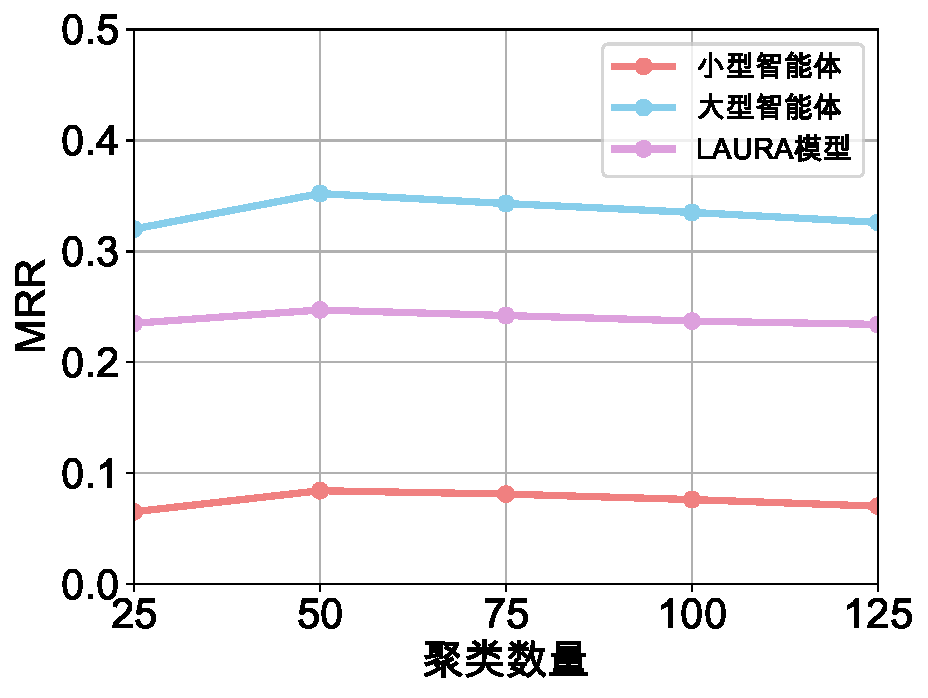
\includegraphics[width=0.3\textwidth]{3_LAURA_layer_FB15K23710.pdf}
    \label{Experiment2_layer_a}
  }
  \subfloat[FB15K-237-20\%数据集] {
    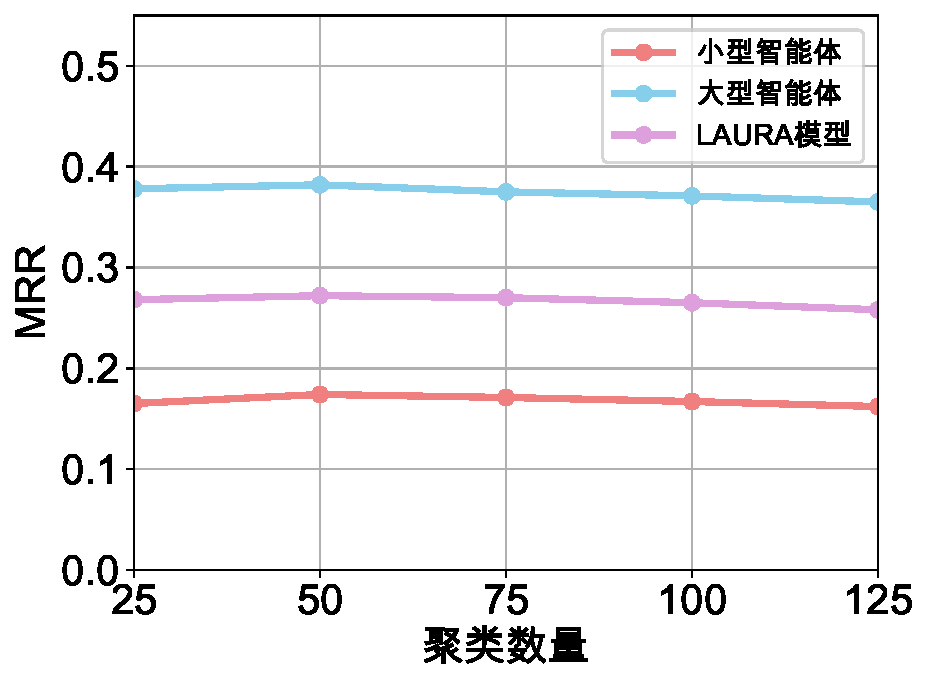
\includegraphics[width=0.3\textwidth]{3_LAURA_layer_FB15K23720.pdf}
    \label{Experiment2_layer_b}
  }
  \subfloat[FB15K-237-50\%数据集] {
    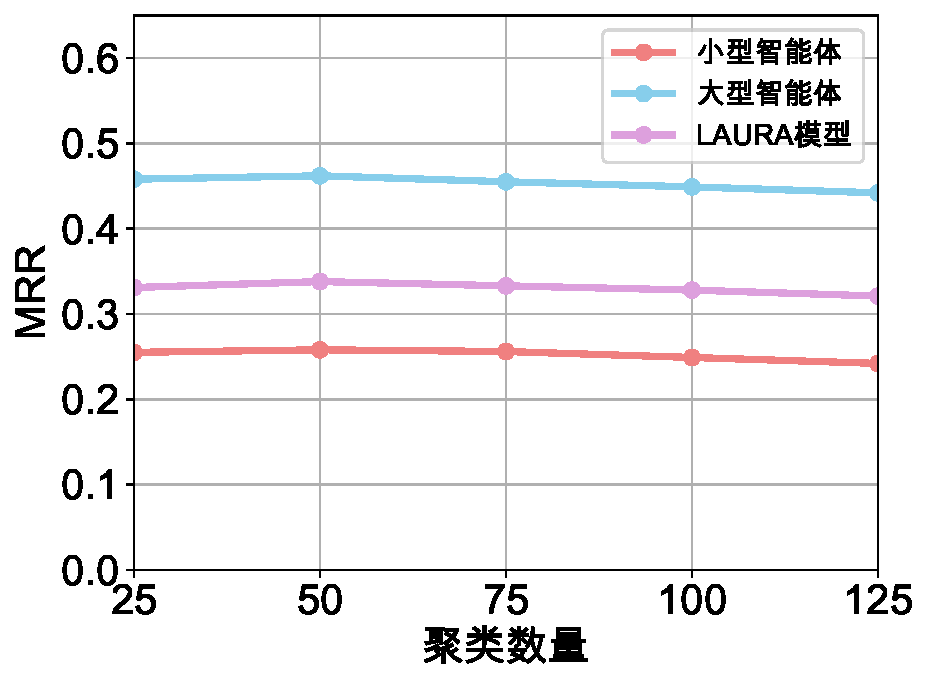
\includegraphics[width=0.3\textwidth]{3_LAURA_layer_FB15K23750.pdf}
    \label{Experiment2_layer_c}
  }
  \caption{聚类数量影响分析}
  \label{Experiment2_layer}
\end{figure}
大型智能体应用了NORMAN模型提供的层次信息进行了聚类知识图谱的构建,因此进行K-Means聚类过程设置的聚类数量$K$对也会影响到LAURA模型的表现。
为了分析聚类数量对LAURA模型的影响,本文在FB15K-237-10\%、FB15K-237-20\%和FB15K-237-50\%三个数据集上开展实验并选择MRR作为评价指标,调整聚类数量$K$并观察模型效果,得到的实验结果如图\ref{Experiment2_layer}所示。
可以发现当设置聚类数量为50时LAURA模型同时在三个数据集上都取得了最好的效果。根据聚类知识图谱的构建过程可以发现,主要是利用了K-Means模型对NORMAN模型提取到实体和关系的半径坐标向量进行聚类,并最终将实体和关系划分为$K$个类别。因此主要原因可以归纳为FB15K-237数据集的知识层数与50最为接近,同时实验采用的三种数据集都是对FB15K-237数据集进行随机采样构建而成,所以知识层数与FB15K-237相同,从而使得模型在三种数据集上都能够在聚类数量为50时取得最好的效果。

\subsubsection{知识推理距离影响分析}
\begin{figure}[t]
  \centering
  \subfloat[FB15K-237-10\%数据集] {
    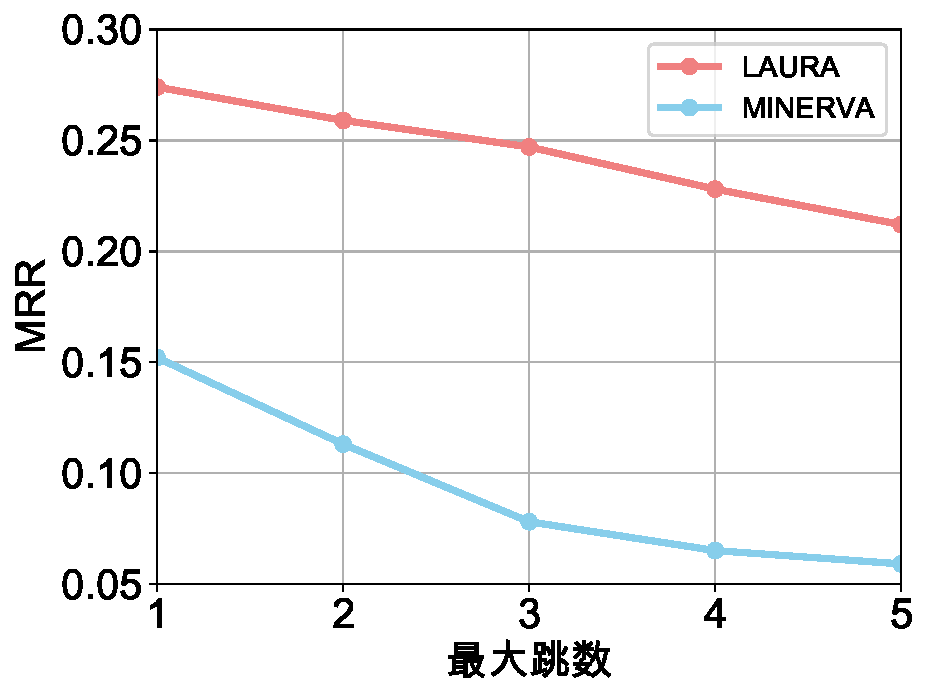
\includegraphics[width=0.3\textwidth]{3_LAURA_hop_FB15K23710.pdf}
    \label{Experiment2_multihop_a}
  }
  \subfloat[FB15K-237-20\%数据集] {
    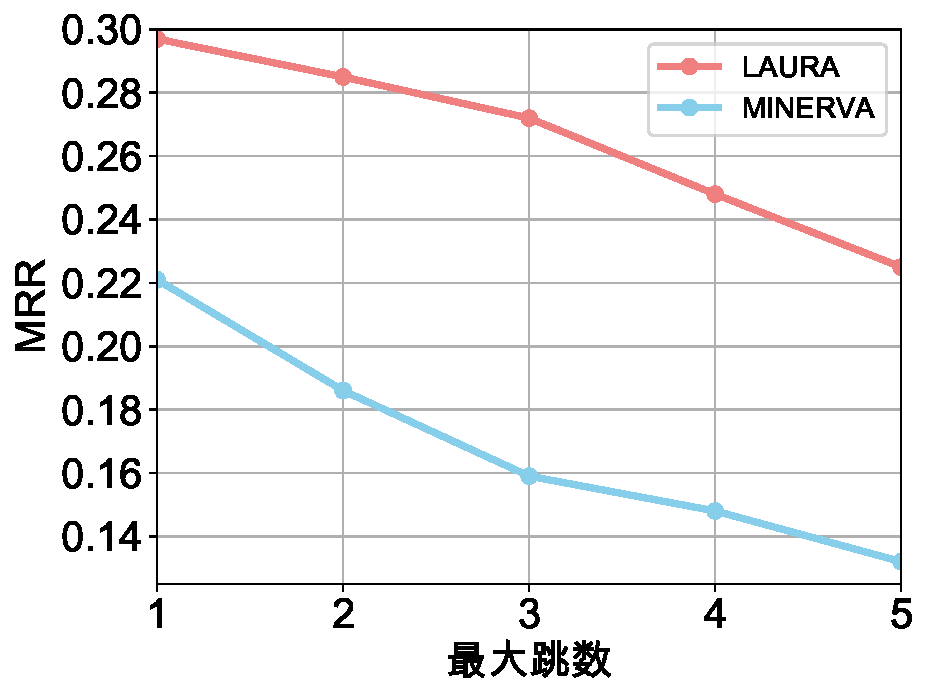
\includegraphics[width=0.3\textwidth]{3_LAURA_hop_FB15K23720.pdf}
    \label{Experiment2_multihop_b}
  }
  \subfloat[FB15K-237-50\%数据集] {
    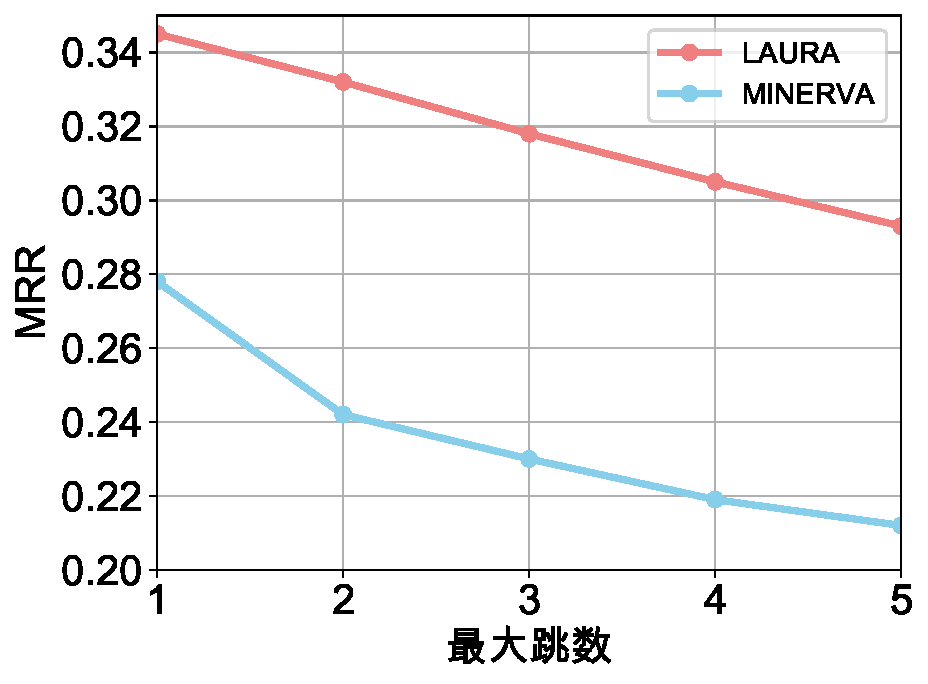
\includegraphics[width=0.3\textwidth]{3_LAURA_hop_FB15K23750.pdf}
    \label{Experiment2_multihop_c}
  }
  \caption{稀疏知识图谱知识推理距离影响分析}
  \label{Experiment2_multihop}
\end{figure}
为了评估模型在稀疏知识图谱上进行知识推理时推理距离的影响,本文在FB15K-237-10\%、FB15K-237-20\%和FB15K-237-50\%三种数据集上开展实验,在实验过程中调整模型的最大跳数$L$并采用MRR作为模型的评价指标。
同时,本文还选择了MINERVA模型作为对比模型进行实验。实验结果如图\ref{Experiment2_multihop}所示。
可以发现MINERVA模型在跳数增加时效果出现了明显的下降。这说明MINERVA模型在进行多跳知识推理时效果不够稳定,容易受到知识推理跳数的影响。
相比之下,本文提出的LAURA模型在三个数据集上均取得了更好的效果,同时模型效果随着知识推理跳数的增长能够实现相对平缓的下降,说明模型的知识推理效果较为稳定。
造成LAURA模型在跳数增加时效果较为稳定的主要原因是LAURA模型采用了双重智能体的方式,在多跳知识推理过程中小型智能体能够获取大型智能体提供的层次信息,从而使得模型能够选择合适的层次进行推理,增加了推理路径的充分性和合理性。同时LAURA模型通过构建扩展动作空间和协作动作空间,实现了对智能体动作空间的扩展,从而能够增强智能体的知识推理能力,并帮助智能体到达目标节点。
而MINERVA模型则缺乏类似的机制,因此容易在推理过程中选择错误层次的节点,同时在稀疏知识图谱上进行多跳推理时容易出现动作空间内可选动作太少的情况,导致了模型在进行长距离多跳知识推理时效果会出现显著下降。

\subsubsection{案例分析}
\begin{table}[t]
  \centering
  \caption{FB15K-237-50\%数据集多跳知识图谱问答案例分析}
  \begin{tabular*}{0.95\textwidth}{@{\extracolsep{\fill}}ccc}
    \toprule[1pt] 
    序号 & 推理问题 & 推理过程 \\ \hline
    1 & $(e_0, Gender, ?)$ & $(e_0 \xrightarrow{Gender} e_a)$ \\
    2 & $(e_0, Nationality, ?)$ & $(e_0 \xrightarrow{PlaceLived} e_1 \xrightarrow{USCounty} e_2 \xrightarrow{Nationality} e_a)$ \\
    3 & $(e_0, ?, e_a)$ & $(e_0 \xrightarrow{Award} e_1 \xrightarrow{Award^{-1}} e_0 \xrightarrow{PerformanceFilm} e_a) $ \\
    \multirow{2}{*}{4} & $(h_{e_0}, r_0, ?)$ & $(h_{e_0} \xrightarrow{r_0} h_{e_1} \xrightarrow{r_1} h_{e_2} \xrightarrow{r_2} h_{e_a})$ \\
    & $(e_0, Profession, ?)$ & $(e_0 \xrightarrow{Award} e_1 \xrightarrow{Award} e_2 \xrightarrow{Profession} e_a)$ \\
    \bottomrule[1pt]
  \end{tabular*}
  \label{Experiment2_CaseStudy}
\end{table}
最后对LAURA模型在多跳知识图谱问答上的任务执行情况进行案例分析。
案例分析过程选择了FB15K-237-50\%数据集上的比较有代表性的多跳知识图谱问答案例,如表\ref{Experiment2_CaseStudy}所示。
为了便于观察,本文将查询语句中的查询三元组提取出来放入表中的推理问题部分,将FB15K-237-50\%数据集中的实体编号信息替换为了$e_i$,同时将聚类节点替换为了$h_{e_i}$,聚类节点间的关系替换为了$r_i$,其中角标$i$表示第$i$跳知识推理过程,同时令角标$a$表示答案。
对表中所获得的结果进行分析,可以发现:
推理样例1说明了LAURA能够解决单跳知识图谱问答问题。在样例中,智能体根据知识图谱中相关信息推测$e_0$的性别并进行排序,最后通过单跳推理获取到了正确的性别$e_a$。
样例2说明了LAURA能够解决多跳知识图谱问答问题。在推理过程中,智能体首先发现知识图谱中存在$(e_0, PlaceLived, e_1)$的知识并进行推理,随后发现存在$(e_1, USCounty, e_2)$的知识并进行推理,最后根据关系$Nationality$对所有候选答案进行排序,得到了最终答案实体$e_a$。需要注意的是,推理过程中的关系$USCounty$对获取最后的答案(国籍信息)起到了重要的提示作用,这说明LAURA智能体状态信息中的历史路径信息具有重要作用,能够在多跳推理过程中提供帮助。
样例3说明了LAURA能够解决查询问题为$(h, ?, t)$类型的多跳知识图谱问答。查询过程中智能体首先根据知识图谱中$(e_0, AwardNominee, e_1)$推测出$e_0$是人名,并根据其他知识推断出$e_a$是电影名称,最后在所有候选关系中选择$PerformanceFilm$作为$e_0$和$e_a$之间的关系,实现了正确的知识推理。
样例4说明了LAURA能够实现小型智能体大型智能体的协作,解决知识图谱问答问题。在该样例中上面一行是大型智能体的推理路径,下面一行则是小型智能体的推理路径,每一步的知识推理中先由大型智能体推理,再由小型智能体推理。在推理过程中,首先大型智能体完成了第一步推理,得到$(h_{e_0}, r_0, h_{e_1})$,随后小型智能体发现实体$e_0$存在知识$(e_0, Award, e_1)$并进行推理。接下来大型智能体在聚类知识图谱中发现存在知识$(h_{e_1}, r_1, h_{e_2})$并进行推理,随后小型智能体参考大型智能体的路径完成了第二步推理,得到了$(e_1, Award, e_2)$。需要注意的是,知识图谱中缺少该知识,也就是说这一知识是小型智能体根据大型智能体的提示加入到协作动作空间中,并通过协作策略网络进行采样得到的新知识。最后,小型智能体通过知识图谱中的有关信息推测获得$e_2$奖项的人物对应的职业并对候选答案进行排序,从而得到了实体$e_0$对应的正确职业$e_a$。

\section{本章小结}
本章主要介绍了基于双重智能体强化学习的知识推理模型LAURA,该模型能够结合知识图谱表示学习模型NORMAN,根据给定的查询问题进行显式的知识推理,返回对应的知识推理路径。
NORMAN模型采用强化学习框架,能够根据知识图谱中的拓扑结构进行多跳推理并生成推理路径,从而实现高可解释性的知识推理。同时,NORMAN模型一种新颖的双重智能体强化学习方法。在知识推理过程中,构建了两种能够相互协作进行知识推理的强化学习智能体,两种智能体能够分别根据知识图谱中的实体和层次信息进行知识推理。同时,采用协作动作空间、协作策略网络和协作奖励等方法,能够帮助两种智能体实现信息交互,指导两种智能体沿相似路径进行知识推理,并帮助彼此到达正确的节点,进而实现高质量和高可解释性的知识推理。此外,模型采用了NORMAN模型的评分函数,从而缓解了知识图谱稀疏造成的智能体动作空间较小的问题,同时通过评分函数计算软奖励提供给没有到达目标节点的推理过程,缓解了在知识图谱上应用强化学习框架存在的奖励稀疏问题,提高了智能体的学习速度和推理能力。
本章首先给出了知识推理的定义,随后介绍了模型概览,并详细介绍了本文提出的基于双重智能体强化学习的知识推理模型的模型与策略,最后在公开数据集上进行了实验,验证了模型的效果。


\chapter{总结与展望}

\section{主要工作总结}
本文的工作主要包括以下两个方面:
\begin{itemize}
  \item [1)]\textbf{提出一种基于图神经网络的知识图谱表示学习模型NORMAN:}
  该方法主要针对知识图谱内的层次信息和邻域信息进行建模,主要包含层次信息提取和图神经网络模型两部分。
  首先为了捕获知识图谱中的层次信息并对不同的实体和关系进行区分,提出了一种基于极坐标系的编码器。该编码器能够将知识编码为极坐标向量的形式,其中半径坐标向量用于捕获知识的层次信息,角坐标向量则用于区分不同类别的知识。
  随后为了捕获知识图谱中的邻域信息,提出了一种图神经网络模型。该模型首先利用层次信息提取过程得到的向量进行全连接层映射,得到模型节点的初始向量,随后通过递归方式实现邻域子图构建和消息传递,并通过消息聚合函数将邻域子图中的消息聚合起来,通过信息更新函数将消息与节点向量相结合,实现节点信息更新。同时在消息传递过程中,对各个邻域节点的消息采用注意力机制,从而区分不同节点的消息贡献程度。
  通过上述方法,NORMAN模型能够有效地捕获知识图谱中的层次信息和邻域信息,进行高质量的知识表示,并能够在知识图谱补全等下游任务中进行应用。
  模型在常用的公开数据集FB15K-237、WN18RR和NELL-995上进行了大量实验,实验结果表明本文提出的NORMAN模型在知识图谱补全任务上的表现优于现有模型,体现了模型能够结合层次信息、因果信息和邻域信息进行知识图谱表示,并能够为知识图谱下游任务提供支持。
  \item [2)]\textbf{提出一种基于双重智能体强化学习的知识推理模型LAURA:}
  该方法主要针对知识图谱中的实体和层次信息进行建模。
  首先为了提高知识推理的可解释性,采用强化学习框架,能够根据知识图谱中的拓扑结构进行多跳推理并生成推理路径,从而实现高可解释性的知识推理。
  随后为了保证知识推理路径的充分性,提出了一种新颖的双重智能体强化学习方法。在知识推理过程中,构建了两种能够相互协作进行知识推理的强化学习智能体,两种智能体能够分别根据知识图谱中的实体和层次信息进行知识推理。同时,采用协作动作空间、协作策略网络和协作奖励等方法,能够帮助两种智能体实现信息交互,指导两种智能体沿相似路径进行知识推理,并帮助彼此到达正确的节点,进而实现高质量和高可解释性的知识推理。
  此外,通过融合知识图谱表示学习模型NORMAN,能够对智能体的动作空间进行扩展,从而缓解了知识图谱稀疏造成的智能体动作空间较小的问题。同时通过利用NORMAN模型的评分函数计算软奖励提供给没有到达目标节点的推理过程,缓解了在知识图谱上应用强化学习框架存在的奖励稀疏问题,提高了智能体的学习速度和推理能力。
  该模型在常用的公开数据集FB15K-237、WN18RR和NELL-995上进行了单跳知识图谱问答实验,并在数据集FB15K-237-10\%、FB15K-237-20\%和FB15K-237-50\%上进行了多跳知识图谱问答实验。实验结果表明,本文提出的LAURA模型在单跳和多跳知识图谱问答上的表现优于现有模型,体现了模型能够结合知识图谱中实体和层次的信息,并通过双重智能体共同进行知识推理的方式,实现高质量知识推理。
\end{itemize}

\section{未来工作展望}
尽管本文实现了一种基于图神经网络的知识图谱表示学习模型NORMAN和一种基于双重智能体强化学习的知识推理模型LAURA,能够在知识图谱补全、单跳知识图谱问答和多跳知识图谱问答等任务上取得优秀的效果,但其中仍然存在一些不足之处。
本文的工作可以在以下几个方面进行改进:
\begin{itemize}
  \item [1)]\textbf{使用双曲空间嵌入模型捕获层次信息:}本文提出的知识图谱表示学习模型NORMAN,采用的层次信息提取方法主要是使用极坐标系编码器在欧氏空间上进行知识图谱编码,并通过极坐标系的半径坐标捕获知识图谱内的层次信息。考虑到双曲空间嵌入模型可以通过超球形状的嵌入空间建模知识图谱的层次结构,在后续的研究工作中可以考虑采用双曲空间嵌入模型建模知识图谱,并捕获知识图谱内的层次信息,例如可以使用庞加莱球模型~\cite{abramowicz2002poincare}等进行知识图谱表示学习。
  \item [2)]\textbf{研究其他多智能体强化学习训练方案:}本文提出的知识推理模型LAURA,在知识图谱问答中构建了两种智能体,能够在两种粒度上进行知识推理,并通过双重智能体强化学习交互模块的协作动作空间、协作策略网络和协作奖励进行信息交流和轨迹协调,从而提高整体知识推理效率和泛化能力。在后续的研究工作中,可以考虑构建其他更多粒度的智能体如邻域子图粒度的智能体,引入额外信息训练智能体,以及采用不同的策略网络和奖励函数训练智能体等。通过研究其他多智能体强化学习训练方案,有助于提高模型效果,同时进一步探索多智能体强化学习的模型构建方式。
  \item [3)]\textbf{采用模仿学习以缓解奖励稀疏问题:}本文提出的知识推理模型LAURA,在大规模稀疏知识图谱上进行知识推理时如果没有到达正确的节点,则通过双重智能体强化学习的协作奖励和知识图谱表示学习模型NORMAN的评分函数提供软奖励的方式获取奖励,从而缓解了奖励稀疏问题。在后续的研究工作中,可以考虑引入模仿学习(Imitation Learning)的方式,基于人类专家的推理路径来对奖励函数进行建模,从而缓解奖励稀疏的问题。例如可以采用VAIL~\cite{pengvariational}的方式对奖励函数进行建模。
\end{itemize}

\acknowledgement
% 岁月如梭,韶光易逝。
% 首先,我想感谢我的恩师汪鹏老师。
% 同时,我想感谢
% 最后,我想感谢
感谢大家的帮助和支持。

\thesisbib{paper}

% \thesisbib{paper}  % 该命令用于生成参考文献,采用 BIBTEX 工具自动生成。为此,需提供.bib 数据库文件名称作为该命令的参数,不需要包含扩展名。
% \bibliographystyle{seuthesix}
% \bibliographystyle{unsrt}
% \bibliography{paper}


\appendix
\resume{作者简介}
周星辰,男,1998年5月30日出生于辽宁抚顺。2016年9月至2020年6月就读于中国地质大学(北京)信息工程学院计算机科学与技术专业并获得工学学士学位。2020年9月至2023年6月就读于东南大学计算机科学与工程学院计算机技术专业并获得工程硕士学位。硕士期间的主要研究方向为知识图谱和自然语言处理。
\begin{flushleft}
  \textit{\large 发表的论文}\\ 
  \relax[1] \textbf{Xingchen Zhou}, Zhe Pan and Peng Wang. Low-dimensional Knowledge Graph Embedding based on Extended Poincaré Ball[C]. In: Proceedings of the 20th International Semantic Web Conference, ISWC (CCF B), 2021.\\
  \relax[2] \textbf{Xingchen Zhou}, Peng Wang, Guozheng Li, Jiafeng Xie and Jiangheng Wu. Weibo-MEL, Wikidata-MEL and Richpedia-MEL: Multimodal Entity Linking Benchmark Datasets[C]. In: Proceedings of the 15th China Conference on Knowledge Graph and Semantic Computing, CCKS (EI), 2021.\\
  \relax[3] \textbf{Xingchen Zhou}, Peng Wang, Qiqing Luo and Zhe Pan. Multi-hop Knowledge Graph Reasoning Based on Hyperbolic Knowledge Graph Embedding and Reinforcement Learning[C]. In: Proceedings of the 10th International Joint Conference on Knowledge Graphs, IJCKG (EI), 2021.\\
  % \relax[3] Peng Wang, Jing Zhou, Yuzhang Liu and \textbf{Xingchen Zhou}. Transet: Knowledge graph embedding with entity types[J]. Electronics 10 (12), 1407.\\

  % ~\\[0pt]
  % \textit{\large 竞赛获奖}\\
  % \relax[1] 2019年ISWC OAEI大赛SPIMBENCH项目第1名
  % \relax[2] 2019年CCKS人物关系抽取大赛第5名
  
  % ~\\[0pt]
  % \textit{\large 获得专利}\\ \relax
  % \relax[1] 一种基于动态知识图谱的无模板通用智能问答方法 (专利号: ZL2019114214475)
\end{flushleft}

\end{document}
